\chapter{Cryptography and Computer Security}
\section{Classical Systems}
{\bf Shannon Theory: } Shannon \emph{entropy} of random variable $X$ is 
$H(X)= - \sum_{i=1}^n P(X=x_i) lg(P(X=x_i))$.
What is the amount of information in a number $n: 0 \le n <2^m$?  
Information learned about 
$Y$ by observing $X$ is $I(Y; X)= H(Y) - H(Y|X)$.  Note $H(Y|X)= -\sum p_X(x) H(Y|X=x)$ which
is generally not equal to $\sum_{X, Y} p_Y(y|x) lg(p_Y(y|x))$.
$H_E= lim_{N \rightarrow \infty} {\frac {H(P^n)} {n}}$.  $H(K|C)= H(M|C)+ H(K|M,C)$.
\\
\\
{\bf Application to cryptography: }
\emph{Perfect secrecy: } $Pr(M|C)=P(M)$.  
\emph{Unicity Theorem: }  Let $H$ be the entropy of the 
source (say English) and let $\Sigma$ be the alphabet.  
Let $K$ be the set of (equiprobable) keys, then $u= {\frac {lg(|K|)} {(lg(|\Sigma|)-H)}}$.
The ``Index of Coincidence,''
$IC(f)= {\frac {\sum {f_i(f_i-1)}} {n(n-1)}}$.
$MC(f, f')= {\frac {\sum {f_i f_{i}'}} {n n'}}$.
\\
\\
{\bf Vigeniere alphabet chaining: }  If $\alpha$ is the mixed plaintext alphabet and
$\beta$ is the mixed cipher alphabet underneath, rearranging with the plain alphabet into
its normal form we get the tableaux:
\begin{center}
\begin{tabular} {|c|c|c|c|}
\hline
1 & 2 & $\ldots$ & n\\
\hline
$\beta(\alpha^{-1}(1))$ & $\beta(\alpha^{-1}(2))$ & $\ldots$ & $\beta(\alpha^{-1}(n))$\\
$\beta(\alpha^{-1}(1)+1)$ & $\beta(\alpha^{-1}(2)+1)$ & $\ldots$ & $\beta(\alpha^{-1}(n)+1)$\\
$\ldots$ & $\ldots$ & $\ldots$ & $\ldots$\\
$\beta(\alpha^{-1}(1)+n-1)$ & $\beta(\alpha^{-1}(2))$ & $\ldots$ & $\beta(\alpha^{-1}(n)+n-2)$\\
\hline
\end{tabular}
\end{center}
Note that the columns have the same sequence of characters as the original rows ---
if plain A corresponds to cipher F and
if plain F corresponds to cipher W then the distance between plain A and plain F is the
same as cipher F and cipher W in the original sequence.
\\
\\
{\bf Heburn: } Five rotors, 
two ratchet controls.  Key: $[i,j,k,m,n]$ and 2 ratchet stepping 
controls at right and left $(l, r)$.  Rightmost ($R_5$) rotor moved after
every enciphered 
letter.  Leftmost ($R_1$) moved when fast rotor reached position specified by $r$.  
$a(m)$ character in line to $R_5$.
When the leftmost rotor hit $l$ the middle ($R_3$) rotor moved one position.  Equation:
$(p)K C^iR_1C^{-i} C^j R_2 C^{-j} C^k R_3 C^{-k} C^m R_4 C^{-m} C^n R_5 C^{-n} L=c$,
$C$ is the cyclic in alphabetical order.  Solution: $c(m)= a(m) C^{(m+p)} R_5 C^{-(m+p)}L$,
$d(m,p)= c(m)L^{-1} C^{(m+p)} R_5^{-1} C^{-(m+p)}$ then 
$d(m,p) R_5^{-1} C^{n-m} R_5=d(n,p)$.  Practical application relies on the IC for the
monoalphabetic substitution (imagine all the input letters are the same).  If 
$i=d(m,p)$, $j=d(n,p)$ and $k=n-m$.  To remove noise, tally
$s'[i,j,k]= \sum_m \sum_n s[i, m, k-m] s[m,j,n]$, this can be iterated.
\\
\\
{\bf Enigma: }
$K$: Keyboard.
$P=(ABCDEFGHIJKLMNOPQRSTUVWXYZ)$.
$N$: First Rotor.
$M$: Second Rotor.
$L$: Third Rotor.
$U$: Reflector.  Note: $U=U^{-1}$.
$i,j,k$: Number of rotations of first, second and third rotors respectively.
$c= (p) P^i N P^{-i} P^j M P^{-j} P^k L P^{-k} U P^k L^{-1} P^{-k} P^j M^{-1} P^{-j} P^i N^{-1} P^{-i}$.
Later military models added plug-board or ``Stecker''($S$):
$$c=(p) S P^i N P^{-i} P^jMP^{-j} P^kLP^{-k} U P^kL^{-1}P^{-k} P^jM^{-1}P^{-j} P^iN^{-1}P^{-i}
S^{-1}.$$
Total key including rotor wiring (in bits):
$67.1 + 3 \times 88.4 = 312.3$.
\\
\begin{figure} 
\center
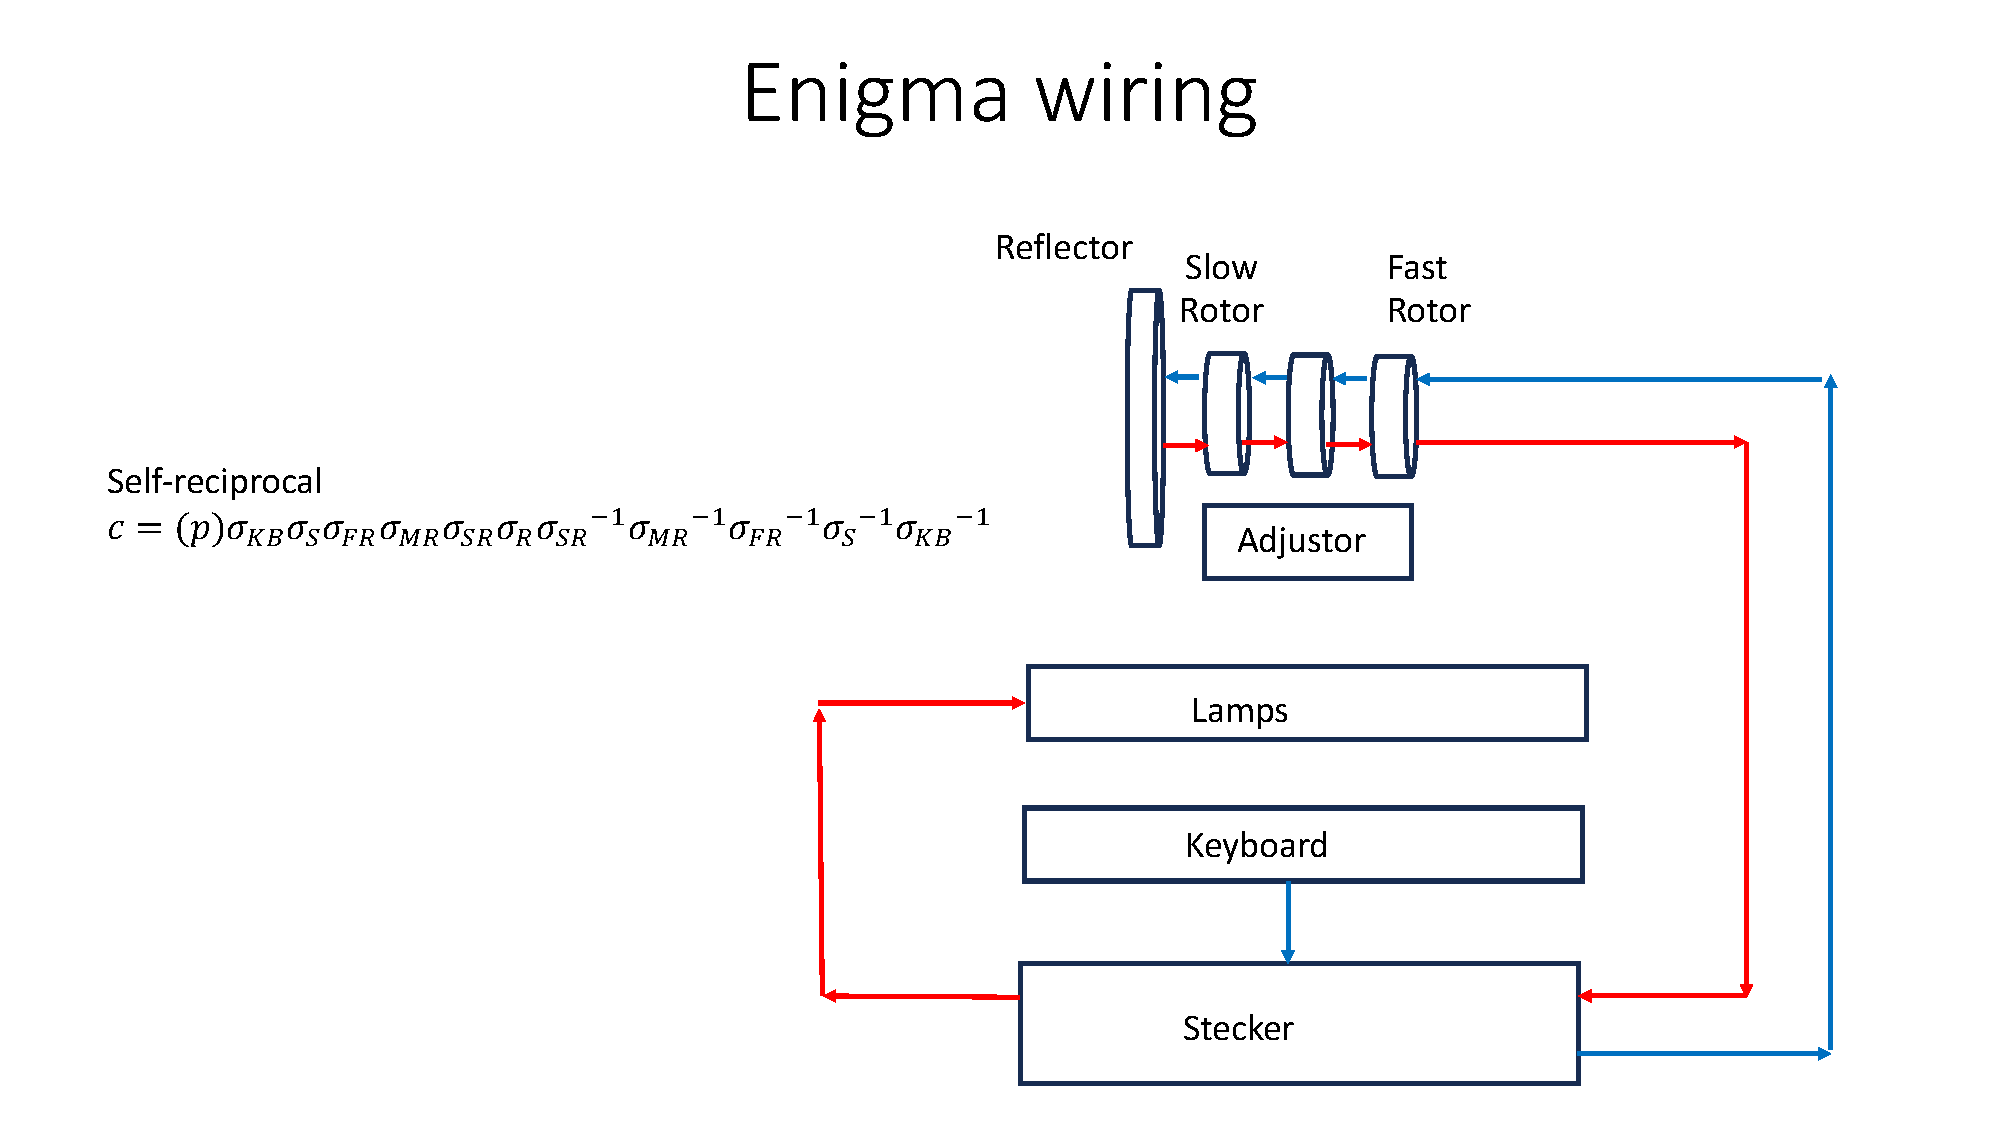
\includegraphics[width=0.8\textwidth,natwidth=642,natheight=610, height=80mm, width=88mm]{Enigma.pdf}
\end{figure}
\emph{Method of Batons (no Stecker):} 
Let $N$ be the fast rotor and $Z$ the combined 
effect of the other apparatus, then,
$N^{-1}ZN(p)=c$ 
at first letter; assuming other rotor doesn't turn,
$P^{-i}N^{-1}P^iZP^{-i}NP^i(p)=c$ or
$ZP^{-i}N(p(i))P^i= P^{-i}NP^i c(i)$.  \emph{Rejewski:}
Let $Q= MLUL^{-1}M^{-1}=Q^{-1}$,
the first 6 permutations (used to encrypt settings twice) are:
$$A=A^{-1}= SP^1NP^{-1}QP^1N^{-1}P^{-1}S^{-1}, B=B^{-1}= SP^2NP^{-2}QP^2N^{-1}P^{-2}S^{-1}$$
$$C=C^{-1}= SP^3NP^{-3}QP^3N^{-1}P^{-3}S^{-1}, D=D^{-1}= SP^4NP^{-4}QP^4N^{-1}P^{-4}S^{-1}$$
$$E=E^{-1}= SP^5NP^{-5}QP^5N^{-1}P^{-5}S^{-1}, F=F^{-1}= SP^6NP^{-6}QP^6N^{-1}P^{-6}S^{-1}$$
Their products and ciphertext ($c_1c_2c_3c_4c_5c_6$) satisfy:
$$AD= SP^1NP^{-1}QP^1N^{-1}P^3NP^{-4} QP^4N^{-1}P^{-4} S^{-1}, (c_1)AD= c_4$$
$$BE= SP^2NP^{-2}QP^2N^{-1}P^3NP^{-5}QP^5N^{-1}P^{-5}S^{-1}, (c_2)BE= c_5$$
$$CF= SP^3NP^{-3}QP^3N^{-1}P^3NP^{-6}QP^6N^{-1}P^{-6}S^{-1}, (c_3)CF= c_6$$
So we can find $AD$, $BE$ and $CF$ after about 80 messages.  To solve for rotors if
$S$ is known.  First note the following theorem.
\\
\\
{\bf Theorem: } If two permutations of the same 
degree consist of disjoint transpositions then their product contains an even number of cycles
of the same length (and conversely). ``Cillies'' (guessed simple indicators like aaa)
align cycles. Let $U=P^{-1}S^{-1}ASP= PNP^{-1}QPN^{-1}P^{-1}$,
$V= P^{-2}S^{-1}BSP^2$, etc, then 
$VW= NP^{-1}N^{-1} (UV)  N P N^{-1}$,
$WX= NP^{-1}N^{-1} (VW)  N P N^{-1}$, etc.
which can be solved for $N$.
\\
\\
Assume we know all rotor wirings and the plaintext for some received ciphertext. 
We do not know plugboard, rotor order, ring and indicator.
\begin{verbatim}
Position   123456789012345678901234
Plain Text OBERKOMMANDODERWEHRMACHT
CipherText ZMGERFEWMLKMTAWXTSWVUINZ
\end{verbatim}
Observe the loop $A[9] \rightarrow M[7] \rightarrow E[14] \rightarrow  A$.
$(E)M_7M_9M_{14}=E$, where $M_i$ is the effect of the machine at position $i$.
British Bombe searched probable text for these loop isomorphisms.  False alarms have probability
${\frac 1 {26}}$ for each independent loop tested.
\section{Public Key Systems}
{\bf RSA: } $n=pq$, choose e, $ed=1 \jmod{\phi(pq)}$, $e$ is often $2^{16}+1$ for efficiency.
\\
\\
{\bf DLP: } Given $g, h$ and $h=g^x$, find $x$.  
{\bf DHP: }  Given $g, a=g^x, b=g^y$, find $z= g^{xy}$.
{\bf DDH: } Given $g \in G, a=g^x, b=g^y, c=g^z$, determine if $z=xy$.  $DDH \le DHP \le DLP$.
\\
\\
{\bf Theorem: } $FACTOR \le SQRT \le FACTOR$.  
If the RSA problem is hard, then RSA is secure under a chosen plaintext attack.  If DHP
is hard, El Gamal is secure under a chosen plaintext attack.
\\
\\
{\bf Finding square roots (mod p): } 
Suppose $({\frac a p})=1$, so that $a$ is a square and let $n$ be a quadratic
non-residue  $\jmod{p}$.  Want to find $x$:
$x^2= a \jmod{p}$.  Set $p-1= 2^{e}q$ and put $b=n^q \jmod{p}$
If $p= 3 \jmod{4}$, $x= a^{\frac {(p+1)} {4 }} \jmod{p}$.
If $p= 5 \jmod{8}$, let
$b=a^{\frac {(p-1)}{4}} = \pm 1\jmod {p}$, then
if $b=1, x= a^{\frac {(p+3)} {8}} \jmod {p}$, otherwise,
if $b= -1, x= (2a)(4a)^{\frac {(p-5)} {8}} \jmod{p}$.
This leaves the hard case, $p=1 \jmod{8)}$.  The algorithm of \emph {Tonelli
and Shanks} solves this case (and the others).
We want $x: x^2= a \jmod {p}$.  Put
$p-1=2^e  q$, $q$, odd.
Choose $n$: $({\frac n p})= -1$; note $n$ is a generator
for the multiplicative group. Set $z= n^q \jmod {p}$ and $b= a^q$.  Since $b^{2^{e-1}}= 1$,
$b$ is a quadratic residue and $b= z^{2k}$ or $bz^{k'}=1$.  Put $x= a^{\frac {q+1} 2} z^{{\frac {k'} 2}}$
then $x^2 = a \jmod{p}$.
\\
The algorithm:\\

$Q= {\frac {(q-1)} 2}$, $z = n^q$,
$y=z$, $r=e$,  $x=a^Q \jmod{p}$, $b=ax^2 \jmod{p}$ and  $x= ax \jmod{p}$.
$x= a^{\frac {q+1} 2} z^{\frac {k'} 2}$ will satisfy $a= x^2$ where $z^k=1$.
Now set $R=2^{r-1}, ab=x^2, y^R= -1, b^R=1$.  Do the following:
\\
\jt loop: \\
\jt\jt  if($b=1$) \\
\jt\jt\jt   return($x$); \\
\jt\jt  Let $M=2^m$. For smallest $m>0: b^M= 1 \jmod{p}$\\
\jt\jt  if($m=r$) \\
\jt \jt \jt return(non-residue);\\
\jt \jt $t= y^{2^{r-m-1}} \jmod{p}$;\\
\jt \jt $y= t^2 \jmod{p}$; \\
\jt \jt $r=m;$ \\
\jt \jt $x=xt;$ \\
\jt \jt $b=by;$ \\
\jt \jt goto loop;
\\
\\
{\bf Theorem: } Factoring $n$ may be equivalent to computing $\phi(n)$ which is equivalent to
finding $d$.\\
\\
{\bf Definitions: }
\emph{Strong primes: }
$p-1$ has a large prime factor $r$,
$p+1$ has a large prime factor $a$,
$r-1$ has a large prime factor $t$.
\emph{Miller-Rabin} has error probability $p= {\frac 1 4}$ as the following shows.
\\
\\
{\bf Definition: } A composite number $n$ is a Carmichael number if $\forall a <n: (a,n) = 1$
we have $a^{n-1} = 1 \jmod{n}$.
\\
\\
{\bf Theorem: } $n \ge 3$ is a Carmichael number iff $n$ is square-free and $(p-1) \mid (n-1), \forall p | n$.
\begin{quote}
\emph{Proof: }
Let $(a, n) = 1$.\\
$\rightarrow$: Suppose $n$ is a Carmichael number. $a^{p-1} = 1 \jmod{p}$ so $a^{p-1} = 1 \jmod{n}$
and $(p-1) \mid (n-1)$.  If $n$ is not square free, $p^k (p-1) \mid \phi(n)$ so,
for some $a$, $a^p = 1 \jmod{n}$ but $a^{p-1} = 1 \jmod{n}$.  Contradiction.
\\
$\leftarrow$: 
Suppose $n$ is square-free and $(p-1) \mid (n-1), \forall p \mid n$. $a^{p-1} = 1 \jmod{p}$.
So $a^{n-1} = 1 \jmod{n}$.
\end{quote}
{\bf Theorem: } If $n \ge 3$ is a Carmichael number, $n$ is divisible by three or more primes.
\begin{quote}
\emph{Proof: } Suppose $n = pq$.  
$(p-1) \mid (pq - 1)$ and
$(q-1) \mid (pq - 1)$. $(p-1)a = pq -1 = pq - q + q-1 = q(p-1) + q-1$ so $(p-1) \mid (q-1)$.
Thus $2(p-1) \geq (q-1)$.  Similarly
$2(q-1) \geq (p-1)$.  This is a contradiction.
\end{quote}
{\bf Theorem: } If $n$ is prime, $n-1 = 2^sd$ $\forall a < n$, then either
$a^d =1 \jmod{n}$ or $a^{2^rd}$ for some $r < s$.
\begin{quote}
\emph{Proof: }
For any $a: (a,n) = 1$, $a^{2^sd} = 1 \jmod{n}$ and the result follows.
\end{quote}
{\bf Theorem: } If $n \ge 3$ is composite then $S= \{x: 1 \leq x < n \}$ has at most
${\frac {n-1} 4}$ non-witnesses.
\begin{quote}
\emph{Proof: }
If there are no non-witnesses, the result holds.  Let $a$ be a non-witness,
$a^{d} = 1 \jmod{n}$ or $a^{2^rd} = -1 \jmod{n}$ for some $r < s$.  In fact,
we can assume $a^{2^rd} = -1 \jmod{n}$ because $a^{d} = 1 \jmod{n}$ implies
$(-a)^{d} = -1 \jmod{n}$.  Let $k$ be the largest $k: a^{2^kd} = -1 \jmod{n}$.
Put $n = \prod_{p \mid n} p^{e_p}$ and $m = 2^kd$.  Define
$J= \{a, a < n, (a,n)=1, a^{n-1} = 1 \jmod{n} \}$,
$K= \{a, a < n, (a,n)=1, a^{n-1} = \pm 1 \jmod{p^{e_p}} \}$,
$L= \{a, a < n, (a,n)=1, a^{m} = \pm 1 \jmod{n} \}$, and
$M= \{a, a < n, (a,n)=1, a^{m} = 1 \jmod{n} \}$.
Thus $ M \subseteq L \subseteq K \subseteq J\subseteq ({\mathbb Z} / (n{\mathbb Z}))^*$.
If $a$ is a non-witness, $a \in L$.  $[K:M] = 2^{\alpha}$ since $x \in K \rightarrow x^2 \in M$.
So $[K:L] = 2^j$.  If $j \geq 2$, we're done.
If $j=1$, $n=pq$ and $n$ is not a Carmichael number, so $[({\mathbb Z} / (n{\mathbb Z}))^* : K] \geq 1$.
$[K:L] =2$ so $[({\mathbb Z} / (n{\mathbb Z}))^* : L] \geq 4$ and we're done.
If $j=1$, $n=p^e, e>1$ so $p(p-1) \mid \phi(n)$ and $[({\mathbb Z} / (n{\mathbb Z}))^* : J] \geq p$.
If $p^e \geq 4$, were done.  The only remaining case is $n = 9$.  The theorem holds for this case as well.
\end{quote}
{\bf El Gamal Crypto: }
For the \emph{El Gamal encryption system}, let $g$ be a generator of $F_{q}^*$.  
A picks $a$ at random,
this is A's secret.  User picks $k$ at random and sends $(g^{k}, Pg^{ka})$.
An \emph{El Gamal Signature} is generated as follows: $g$ is a primitive element
${\mathbb Z}_{p}^{*}$. $(p, g , y=g^x )$ are public, $x$ is secret.  To sign
$m$, pick $k$: $1 \leq k \leq p-2$ with $(k, p-1)= 1$.
$sig_K (m, k) =(r, s)$, $r=g^k$, $s= k^{-1}(m-xr)$.
$ver_k (m, r, s)$ is true iff $y^{r}r^{s}==g^m$.
Note: $k$ must be different for each signature and $m$ must be a hash.
\emph{Recommended parameters:} $>768$ bits.
There is an existential forgery if hash isn't used in El Gamal.
For key elements, $(\langle {\mathbb Z}_p \rangle, g, a)$, pick 
$(u, v)$, $r= g^u g^v = g^{u+av}$.
$s= -rv^{-1} \jmod{p-1}$, $M=su$.  Note that $t=r^s y^r=g^{su}$.
\\
\\
{\bf Diffie Hellman Key Exchange: }
The \emph{Diffie Hellman} key exchange scheme works as follows: Let $g$ be a generator of $F_{q}^*$.
A generates $a \in F_{q}^*$ at random and transmits $g^{a}$,
B generates $b \in F_{q}^*$ at random
and transmits $g^{a}$,  they use $g^{ab}$ as key.
\\
\\
{\bf Blinding and E-cash: } Let $M$ be a note or check.  To blind, generate random
$k$.  Let $(e, d, n)$ be the bank's key and $H$, a hash.  Send bank $r=H(M)k^e$.
Bank sends back $r^d$, now multiply by $k^{-1}$.  For fraud resistant
protocol,
do this for a bunch of $k_s$'s.  Bank signs one of them.  
\\
\\
{\bf DSA: } Pick $p, q$, $2^{159}<q<2^{160}$, $2^{511+64t} < p < 2^{512+64t}$, $0 \le t \le 8$ with
$q|(p-1)$.  
Let $x$ be a primitive root $\jmod{p}$.  Set $g= x^{{\frac {p-1} q}}>1 \jmod{q}$. 
Finally,
pick $a$ at random and set  $A= g^a \jmod{p}$.
$p, q, g, A$ are public, $a$ is secret.  To sign $M$:
generate random $k: k<q$.  Set $r= g^k \jmod{q}$ and compute
$s= k^{-1} (h(M) + xr) \jmod{q}$, where $h$ is a cryptographic hash.  
\emph{Signature} is $(r, s)$.
\emph{To verify:}
$u_1= s^{-1} h(M) \jmod{q}$,
$u_2= s^{-1} r \jmod{q}$,
$v= g^{u_1} g^{u_2} \jmod{p} \jmod{q}$.  If $v=r$, it
verifies.  Unlike El Gamal signature, $s$ does not carry full information about
$p$ (only $\jmod{q}$) and since $q$ is large, the Pohlig-Hellman attack is harder.
\\
\\
{\bf Montgomery Arithmetic: }
Suppose $(R, n)=1$; think of $R= 2^r$, $n < 2^r$.
$R R' - n n' = 1$ (i.e.- $n'= -n^{-1} \jmod{R}$). \\
\emph{Theorem: }  If $0 \leq t < nR$ and $u=tn' \jmod{R}$ then
$R \mid (t+un)$ and for $x= {\frac {(t+un)} R}$, $x= t R^{-1} \jmod{n}$ and
$0 \leq x < 2n$.\\
\\
${\overline a}= a r \jmod{n}$.
$r r' - n n' = 1$. \\
\jt MontPro(${\overline a}, {\overline b}$) \\
\jt \jt $t= {\overline a} {\overline b}$; \\
\jt \jt $u= tn' \jmod{R}$; \\
\jt \jt $x= {\frac {un+t} R}$; \\
\jt \jt if($x>n$)  \\
\jt \jt \jt $x-=n$; \\
\jt \jt return($x$); \\
\\
\jt MontMult($a,b,n$): Compute $n'$ ;\\
\jt \jt ${\overline a}= a r \jmod{n}$;\\
\jt \jt ${\overline b}= b r \jmod{n}$;\\
\jt \jt ${\overline x}= MontPro({\overline a}, {\overline b})$;\\
\jt \jt $x= MontPro({\overline x}, 1)$;\\
\jt \jt return($x$).
\\
\\
{\bf NAF: } Let $k= \sum_{j=0}^l s_j 2^j, s_j \in \{0, 1\}$. NAF form is
$k= \sum_{j=0}^{l+1} c_j 2^j, c_j \in \{-1, 0, 1\}$, conversion is achieved
by following algorithm:\\
\jt $c_0 =0;$\\
\jt $for(j=0; j \le l; j++) \{$\\
\jt \jt $c_{j+1}= \lfloor (k_j + k_{j+1} +c_j) /2 \rfloor;$ \\
\jt \jt $s_{j}= k_j + c_j -2 c_{j+1}; \\
\jt \}$
\\
\\
{\bf AMD-64 3Ghz dual core timings: }
\begin{center}
\begin{tabular} {|l|rrr||l|rrr|}
\hline
{\bf Algorithm} & {\bf KSize} & {\bf T($\mu$-sec)} & {\bf Cycles} &
{\bf Algorithm} & {\bf KSize} & {\bf T($\mu$-sec)} & {\bf Cycles} \\
\hline
ECDSA-SIGN & 256 & 4942 & 14,827,000 &
ECDSA-VERIFY & 256 & 9,848 & 29,546,000 \\
ECDSA-SIGN & 384 & 13,000 & 38,860,000 &
ECDSA-VERIFY & 384 & 25,900 & 77,639,000 \\
ECDSA-SIGN & 521 & 29,500 & 88,287,000 &
ECDSA-VERIFY & 521 & 58,900 & 176,524,000 \\
\hline
\end{tabular}
\end{center}
\begin{center}
\begin{tabular} {|l|rrr||l|rrr|}
\hline
{\bf Algorithm} & {\bf KeySize} & {\bf T($\mu$-sec)} & {\bf Cycles} &
{\bf Algorithm} & {\bf KeySize} & {\bf T($\mu$-sec)} & {\bf Cycles} \\
\hline
DSA-SIG & 512 & 1,077 & 3,233,000 &
DSA-VERIFY & 512 & 2,142 & 6,427,000 \\
DSA-SIG	& 768 & 2,332 & 6,999,000 &
DSA-VERIFY & 768 & 4,641 & 13,924,000 \\
DSA-SIG	& 1024	& 4,027 & 12,083,000 &
DSA-VERIFY	& 1024 & 8,015 & 24,047,000 \\
\hline
\end{tabular}
\end{center}
\begin{center}
\begin{tabular} {|l|rrr|l|rrr|}
\hline
{\bf Algorithm} & {\bf KeySize} & {\bf T($\mu$-sec)} & {\bf Cycles} &
{\bf Algorithm} & {\bf KeySize} & {\bf T($\mu$-sec)} & {\bf Cycles} \\
\hline
RSA-SIGN & 1024 & 3,488 & 10,465,000 &
RSA-VERIFY	& 1024 & 168 & 505,000 \\
RSA-SIGN & 2048 & 22,905 & 68,717,000 &
RSA-VERIFY	& 2048 & 608 & 1,825,000 \\
RSA-SIGN & 3072 & 72,494 & 217,491,000 &
RSA-VERIFY & 3072 & 1,340 & 4,021,000 \\
RSA-SIGN & 4096 & 168,548 & 505,664,000 &
RSA-VERIFY & 4096 & 2,363 & 7,091,000 \\
\hline
\end{tabular}
\end{center}
\begin{center}
\begin{tabular} {|rrr||rrr|}
\hline
{\bf Algorithm} & {\bf KeySize} & {\bf T(sec)} & {\bf Algorithm} & {\bf KeySize} & {\bf T(sec)} \\
\hline
RSA KeyGen & 1024 & .37 & ECC KeyGen & 160 & .0053 \\
RSA KeyGen & 2048 & 3.5 & ECC KeyGen & 224 & .0056 \\
RSA KeyGen & 3072 & 11.2 & ECC KeyGen & 256 & .0067 \\
\hline
\end{tabular}
\end{center}
{\bf McEliece Cryptosystem: }  Bob chooses $G$, an $[n,k,d]$ linear code,
$G_1= SGP$ where $P$ is an $n \times n$ permutation matrix and $S$ is a $k \times k$
invertible matrix.  To send a message to Bob, Alice adds an error, $e$, of weight $t$,
$y=xG_1+e$.  To decrypt, (1) compute $y_1= yP^{-1}= xSG+e_1$; (2) apply error
decode to $y_1$ to get $x_1$; (3) compute $x_0: x_0G= x_1$; (4) compute $x=x_0S^{-1}$.
Want $d$ to be large.  For example, use Goppa code ($n=2^m, d= 2t+1, k= n=mt$): 
$m=10, t=50$ to get $[1024, 524, 101]$.
\\
\\
\section{Symmetric Key Systems}
{\bf Modes: }
\emph{CBC: } $y_0 = IV$, $y_i = E_K (x_i + y_{i-1})$.
\\
\emph{OFB: } $z_0 = IV$, $z_{i+1} = E_K (z_i )$, $y_i = x_i + z_{i}$.
\\
\emph{CFB: } $y_0 = IV$, $z_i = E_K (y_{i-1})$, $y_i = x_i + z_i $.
\\
\emph{CTR: } $z_i = E_K (Nounce||ctr)$, $y_i = x_i \oplus z_i $.
\\
\emph{HMAC: } $(K,m) \mapsto h( (K \oplus a) || h(K \oplus b) || m)$.
\\
\emph{GCM: } $F=GF(2^{128}), p(x)= 2^{128}+x^7+x^2+x+1$, $(z_0 , y_0)= (IV,0^{128})$,
$(z_1, y_i) \mapsto (z_{i+1}, y_{i+1})$ by $z_{i+1}= \pi_i(z_i)$, if $\pi_i(x)=0$,
$z_i \oplus y_i$ otherwise and $y_{i+1} = y_i >> 1$ if $LSB(y_i)=0$ otherwise
$y_{i+1}= (y_i>>1) \oplus R$, $R= [11100001 || 0^{120}$.  
Define $X \cdot Y= (z_{128}, y_{128})$.
$inc_s(X)=MSB_{len(X)-s}(X) || [int(LSBs(X))+1 \jmod {2^s}]_s$.
$GHASH_H(X), len(X)=128m$:
$H = E_K(0^{128})$. $Y_0 = 0^{128}$, $Y_{i+1}= (Y_{i} \oplus X_{i+1}) \cdot H$.
return $Y_m$.
\\
\emph{GCTR: }
$GCTR_K (ICB, X)$: If $X$ is the empty string, then return the empty string as $Y$.
$n= \lceil (len(X)/128 \rceil$.  Let $CB_1 = ICB$, $CB_i= inc_{32}(CB_{i-1}, i= 1 \ldots n$.
$Y_i= X_i \oplus E_K(CB_i)$.  ${Y_n}^*= {X_i}^* E_K(CB_i)$.  return $Y$.
\\
\emph{GCM-AES: }
$GCM-AE_K (IV, P, A)$: $H = E_K(0^{128})$.  If $len(IV)=96$, $J_0 = IV || 0^{31} ||1$.
If $len(IV) \ne 96$, let $s = 128 \lceil len(IV)/128 \rceil-len(IV)$, and let
$J_0=GHASH_H(IV||0^{s+64}||len(IV)^{64})$.
$C=GCTR_K(inc_{32}(J0), P)$.  Let $ n $ Define 
$S = GHASH_H (A || 0^v || C || 0^u || len(A)^{64} || len(C)^{64}$).  $T=MSB_t(GCTR_K(J_0,S))$.
return $(C, T)$.
\\
\\
{\bf Definitions:}
\emph{Recurrence for LFSR of length $k$:} $s_j= c_1 s_{j-1} + \ldots c_k s_{j-k}$.
\emph{Hamming weight:} $w_H(x)= \# \{n: x_n \ne 0 \}$.  
\emph{Modular weight:} $w_M(x)= |x'|$ where 
$x'=x \jmod{2^n}$ and $-2^{n-1} < x' \le 2^{n-1}$.
\emph{NAF weight:} $w_{NAF}(x) = \# \{ i<n: \alpha_i \ne 0 \}$. 
$\Delta^{\oplus}(x,y)$, $\Delta^{+}(x,y)$, $\Delta^{\pm}(x,y)$ are the xor, modular and
signed differences respectively.  \emph{Distortion for map $\varphi$:} 
$D(\varphi, d_1, d_2)=
sup_{x\ne y} {\frac {d_2(\varphi(x), \varphi(y))} {d_1(x,y)}}
sup_{x\ne y} {\frac {d_1(x,y)} {d_2(\varphi(x), \varphi(y))}}$.
$f(x_1, \ldots, x_n)$ is \emph{$m$-correlation immune} if
$I(f(x_1, \ldots, x_n); x_{i_1}, \ldots , x_{i_m})=0$ for any choice of the
$i_k$.  This happens when the boolean spectrum of $F(w)$ is $0$ when
$w$ has weight $\le m$.  
\\
\\
{\bf Definition:}
The \emph{connection polynomial} for $L_n({\vec s})$ is
$c(x)= 1 + c_1 x + \ldots + c_l x^l$ with $c(x)=0$ if $L_n({\vec s})=0$.  
Define $d_n$ as
$n$th discrepancy, suppose $m$ is the position of change of length in minimal generating
LFSR. $L_m({\vec s}) \le L_n({\vec s})$ and $L_{m+1}({\vec s})= L_n({\vec s})$.  
The recurrence is
$c^{(n+1)}(x)= c^{(n)}(x) -d_n {d_m}^{-1} x^{n-m} c^{(m)}(x)$.  
The synthesis algorithm is $O(n^2)$.
\\
\\
{\bf Theorem:} A LFSR of length $k$ has maximal period ($K=2^k-1$) iff its connection 
polynomial is \emph{primitive}.
\begin{quote}
\emph{ Proof: }
Let $G(x)= a_0 + a_1 x + a_2 x^2 + \ldots + a_{m-1} x^{m-1} + \ldots$,
$a_m= c_1 a_{m-1} + \ldots + c_m a_1$, etc.  We get a recurrence yielding
${\frac {K} {1-c(x)}}$, $f(x)= 1-c(x)$.  If sequence is $p$,
$G(x)= 
(a_0 + a_1 x + \ldots + a_{m-1} x^{m-1}) +
(a_0 + a_1 x + \ldots + a_{m-1} x^{m-1}) x^p + \ldots =
{\frac {(a_0 + a_1 x + \ldots + a_{m-1} x^{m-1})} {1-x^p}} = {\frac {K} {(f(x))}}$.
\end{quote}
{\bf Theorem:}
Let $M_{j,k}(x)=
\left(
\begin{array}{ccccc}
x_{j} & x_{j+1} & x_{j+2} & ... & x_{j+k-1}\\
x_{j+1} & x_{j+2} &x_{j+3} & ... & x_{j+k}\\
... & ... & ... & ... & ... \\
x_{j+k-1} & x_{j+k} &x_{j+k+1} & ... & x_{j+2k-2}\\
\end{array}
\right)$. 
If $\langle x_i \rangle$ is generated by an LFSR of length $N$ but not one shorter then
$det(M_{j,N}(x))=1$ and
$det(M_{j,n}(x))=0, n>N$.  If $x_{n+m}= c_0 x_n + \ldots + c_{m-1} x_{n+m-1}$ and
$c(x)= x^m +c_{m-1} x^{m-1} + \ldots + c_0$, the associated connection
polynomial, is irreducible,
then the sequence repeats at an interval of $k= 2^m -1$.
\\
\\
{\bf Massey's Lemma:} If $L_n({\vec s})$ generates 
$\langle s_0, \ldots , s_{n-1} \rangle$ but not
$\langle s_0, \ldots , s_{n} \rangle$ then 
$L_{n+1}({\vec s}) \ge max(L_n({\vec s}), n+1-L_n({\vec s}))$.  
\begin{quote}
\emph{Proof:}
Suppose $L$ generates $\langle s_0 , s_1 , \ldots , s_{n-1} \rangle$ but not
$\langle s_0 , s_1 , \ldots , s_{n} \rangle$ and let $L'$ with
$L_{n+1}'({\vec s})= l'$ then $l' \ge n+1-l$.  Proof.  If $l \ge n$,
$l' \ge 1$ so it's true.  If $l<n$, let $c_i$ be the coefficients of $L$ and
$c_i'$, the coefficients of $L'$.  
$s_j + \sum_{i=1}^l c_i s_{j-i}=0$ for $j= l, l+1, \ldots , n-1$ but not for $j=n$ and
$s_j + \sum_{i=1}^{l'} c_i' s_{j-i}=0$ for $j= l', l'+1, \ldots , n$  so
$-\sum_{i=1}^l c_i s_{j-i}= \sum_{i=1}^l c_i \sum_{k=1}^{l'} c_k' s_{n-i-k}$
Switching the
order of summation, the second sum is $s_n$  which is a contradiction.
\end{quote}
{\bf Berlekamp-Massey:} Given $s_1 , s_2 , \ldots , s_{n-1}$
output linear complexity $L$.
\begin{enumerate}
\item $C(x)= 1, L= 0, m=-1, b(x)= 1, n= 0$.
\item $d= S_n + \sum_{i=1}^L c_i s_{n-i}$.
\item If ($d==1$) $t(x)= c(x), c(x)+= b(x)x^{n-m}$)
if($L \leq {\frac n 2}$)
$L= n+1-L, m=n, b(x)= t(x)$
\item $n= n+1$;
\end{enumerate}
\begin {multicols} {2} {
\begin {verbatim}
RC4Init() {
    for (i=0; i<256; i++)
        s[i]= i;
    fill k[] with key repeating 
         as necessary;
    j= 0;
    for(i = 0; i<256; i++) {
        j= (k[i]+s[i]+j) (mod 256); 
        swap(s[i], s[j]);
        }
    i= 0;
    j= 0;
    }

byte Next() {
    i= (i+1) (mod 256);
    j= (j+s[i]) (mod 256);
    swap(s[i], s[j]);
    return(s[(s[i]+s[j]) (mod 256)]);
    }
\end{verbatim}
}
\end {multicols}
Let $\Lambda(s^n)$ be the associated \emph{linear complexity}
of the sequence $\langle s_i \rangle$ of
length $n$ and $N_n(L)$ be the number of sequences of length $n$ with linear complexity $L$,
then $N_n(L) = 2 N_{n-1}(L) + N_{n-1}(n-L)$, if $n \ge L > {\frac n 2}$;
$N_n(L) = 2 N_{n-1}(L)$, if $L = {\frac n 2}$; and,
$N_n(L) = N_{n-1}(L)$, if ${\frac n 2} \ge L \ge 0$. So
$N_n(L)= 2^{min(2n-2L, 2L-1)}$, if $n \ge L >0$,
$N_n(L)= 1$, if $n \ge L = 0$.  
$E(\lambda(s^n))= {\frac n 2} + {\frac {4+R_2(n)} {18}}- 2^{-n}({\frac n 3} + {\frac 2 9})$,
$Var(\Lambda(s^n))= {\frac {86} {81}}$.
\\
\\
{\bf Shrinking Generator:}  Take two LFSR: $LFSR_1$ and $LFSR_2$
synchronously clocked.  Use $LFSR_2(t)$ in stream when $LFSR_1(t)=1$.
Take $LFSR_i(t)= x_i(t)$ for $i=1,2, \ldots , n$
use $f(x_1(t), x_2(t) , \ldots , x_n(t))$ where $f$ is non linear.  For $k$ stage
shift register design, where stage $i$ has $n_i$ bits of state, keysearch takes
$2^{n_0 + n+1 + \ldots + n_{k-1}}$ while correlation attack takes
$2^{n_0} + 2^{n+1} + \ldots + 2^{n_{k-1}}$.
\emph{Example:}
The Geffe combiner is
$f(x,y,z)= xy \oplus yz \oplus z$, $f(x,y,z)=x$ with $p={\frac 3 4}$. 
\\
\\
{\bf ANSI 9.17 random stream generator:}
$I=E_k(D)$.
$x_i= E_k(I \otimes s)$ and
$s= E_k(x_i \otimes s)$.
\\
\\
{\bf FIPS 186 One Way Function (OWF):} $t$, $c$ 160 bits.  Output $G(t,c)$ where
$t= H_1 || H_2 \ldots || H_5$.  Pad $c$ with $0$s to get 512 bit
block $X$.  Break $X$ into 16 32 bits words $x_0, \ldots, x_{15}$ and
set $m= 1$, apply iterative step of SHA-1.

\begin{multicols} {2} {

\begin{verbatim}
Dual Elliptic Curve RNG
  s[0] in [0,1, ..., #E-1]
  output 240 bits
  for(i=1 to k {
    s[i]= x(s[i-1]P);
    r[i]= lsb[240] x(s[i]Q);
    }
  return(r[1] ... r[k]);
\end{verbatim}


\begin{verbatim}
// State for Hash_DRBG
  V	// seedlen bits
  C	// seedlen bits
  reseedCtr 
\end{verbatim}

\begin{verbatim}
Hash_DRBG_Instantiate(entBitsIn, nonce, 
                      extraEnt)
  seedBits= entBitsIn||nonce||extraEnt;
  seed= Hash_df(seedBits, seedlen);
  V= seed;
  C= Hash_df((0x00||V), seedlen);
  reseedCtr= 1;
  return;
\end{verbatim}

\begin{verbatim}
Hash_DRBG_Reseed(entBitsIn, addInBits)
  seedBits= 0x01||V||entBitsIn||addInBits;
  seed= Hash_df(seedBits, seedlen);
  V= seed;
  C= Hash_df((0x00||V), seedlen);
  reseedCtr= 1;
  return;
\end{verbatim}

\begin{verbatim}
Hash_DRBG_Generate(numReqBits, addInBits)
  if(reseedCtr>reseedInterval) then 
       Reseed;
  if(addInBits!=NULL)
     w= Hash(0x02||V||addInBits);
     V=(V+w) mod 2**seedlen;
  returnedBits= Hashgen(numReqBits, V);
  H= Hash(0x03||V);
  V=(V+H+C+reseedCtr) mod 2**seedlen;
  reseedCtr= reseedCtr+1;
  return returnedBits;
\end{verbatim}

\begin{verbatim}
Hashgen(numReqBits, V)
  m= reqNumBits/outlen;
  data= V;
  W= NULL;
  for i= 1 to m
    w= Hash(data);
    W= W||w;
    data= (data+1) mod 2**seedlen;
  returnedBits= Leftmost numReqBits
                  bits of W;
  return returnedBits;
\end{verbatim}

\begin{verbatim}
Hash_df(inBits, numRetBits):
  temp= NULL;
  m= numRetBits/outlen;
  counter= 8-bit representation of 1;
  for i= 1 to len do
    temp= temp|| Hash(counter||
            numRetBits||inBits);
    counter= counter+1;
  reqBits= Leftmost numRetBits of temp;
  return reqBits;
\end{verbatim}



\begin{verbatim}
// State for CTR_DRBG
    V	// outlen bits
    C	// keylen bits
    reseedCtr 
    nStrength
    fPrediction
\end{verbatim}

\begin{verbatim}
CTR_DRBG_Update(provided_data, Key, V):
  temp= NULL;
  while(len(temp)<seedlen) do
    V=(V+1) mod 2**outlen;
    outBits= blockEncrypt(Key, V);
    temp= temp||ouput_block;
  temp= Leftmost seedlen bits of temp;
  temp= temp^provided_data;
  Key= Leftmost keylen bits of temp;
  V= Rightmost outlen bits of temp;
  return Key and V;
\end{verbatim}

\begin{verbatim}
// Full Entropy
CTR_DRBG_Instantiate(entBitsIn, extraEnt):
  // Ensure that the length of 
  // extraEnt is seedlen bits. 
  temp= len(extraEnt);
  if(temp<seedlen))
    extraEnt= extraEnt||
                [seedlen-temp] bits of 0;
  seedBits= entBitsIn^extraEnt;
  Key= [keylen] bits of 0;
  V= [outlen] bits of 0;
  (Key, V)= Update (seedBits, Key, V);
  reseedCtr= 1;
  return;
\end{verbatim}

\begin{verbatim}
// Derivation function required
CTR_DRBG_Instantiate(entBitsIn, extraEnt):
  seedBits= entBitsIn||nonce||extraEnt;
  seedBits= Block_Cipher_df(seedBits, seedlen);
  Key= 0 of[keylen];
  V= 0 of[outlen];
  (Key, V)= Update (seedBits, Key, V);
  reseedCtr= 1;
  return;
\end{verbatim}

\begin{verbatim}
// Full entropy
CTR_DRBG_Reseed(entBitsIn, addInBits):
  temp= len(addInBits);
  if(temp<seedlen), then 
      addInBits= addInBits||
           [seedlen-temp] bits of 0;
  seedBits= entBitsIn^addInBits.;
  (Key, V)= Update (seedBits, Key, V);
  reseedCtr= 1;
  return;
\end{verbatim}

\begin{verbatim}
// Derivation Function Required
CTR_DRBG_Reseed(entBitsIn, addInBits):
  seedBits= entBitsIn||addInBits;
  seedBits= Block_Cipher_df(seedBits,
                            seedlen);
  (Key, V)= Update (seedBits, Key, V);
  reseedCtr= 1;
  return;
\end{verbatim}

\begin{verbatim}
CTR_DRBG_Generate(numReqBits, addInBits):
    if reseedCtr>reseedInterval, then 
            reseed;
    if(addInBits!=NULL)
        temp= len(addInBits);
    if(temp<seedlen))
        addInBits= addInBits||
                 [seedlen-temp] bits of 0;
        (Key, V)= Update (addInBits, Key, V);
    else 
      addInBits= [seedlen] bits of 0;
   temp= NULL;
   while(len(temp)<numReqBits) do:
     V=(V+1) mod 2**outlen;
     outBits= blockEncrypt(Key, V);
     temp= temp||outBits;
   returnedBits= Leftmost numReqBits of temp;
   // Update for backtracking resistance.
   (Key, V)= Update(addInBits, Key, V);
   reseedCtr= reseedCtr+1;
   return returnedBits; 
\end{verbatim}

\begin{verbatim}
BCC(Key, data):
  CV= [outlen] bits of 0;
  n= len(data)/outlen;
  Split the data into n blocks of outlen bits 
       forming block[1] to block[n];
  for i= 1 to n do
    inBlock= CV^block[i];
    CV= blockEncrypt(Key,inBlock);
  outBits= CV;
  Return outBits;
\end{verbatim}

\begin{verbatim}
Block_Cipher_df(numRetBits, inBits)
  if(numRetBits>maxNumBits), then 
    return ERROR;
  L= len(inBits)/8;
  N= numRetBits/8;
  S= L||N||inBits||0x80;
  // Pad S with zeros, if necessary.
  while(len(S) mod outlen) != 0
       S= S||0x00;
  temp= NULL;
  i= 0;
  K= Leftmost keylen bits 
         of 0x00010203...1D1E1F.
  while len(temp)<keylen+outlen)
    IV= i||[outlen-len(i)] bits of 0;
    temp= temp||BCC(K,(IV||S));
    i= i+1;
  K= Leftmost keylen bits of temp;
  X= Next outlen bits of temp;
  temp= NULL;
  while len(temp)<numRetBits
    X= blockEncrypt(K, X);
    temp= temp||X;
  reqBits= Leftmost numRetBits of temp;
  return reqBits;
\end{verbatim}
MGF property:  Given no input and partial output, remaining output is unpredictable.
\begin{verbatim}
mgf1(mSeed, nLen)
1. if (mLen>2^32), return error
2. T= ||;
3. uL= ceiling(mLen/hLen), 
   // hLen is length of hash used
4. for(c=0; c<uL;c++)
       T= t|| h(mSeed || c);
5. output leading bits
\end{verbatim}
\begin{verbatim}
PSS-Encode(M, emBits, salt, sLen)
// M- message
// emBits- bits of EM >= 8 hLen + 8 sLen + 9
1. emLen= ceil(enBits/8);
2. if (l(M)> largest message), return error;
3. mH= h(M)
4. if( emLen < hLen+sLen+2 ), return error;
5. M'= (0x00)^8 || mH || salt
6. H= h(M');
7. DB= (0x00)^(emLen-hLen-sLen-2) 
       || 0x01 || salt
8. dbMask= mgf(H, emLen-hLen-1);
9. maskedDB= DB^dbMask;
10. Clear leftmost 8*emLen-emBits in maskedDB
11. EM= maskedDB || H || 0xbc
12. return EM;
\end{verbatim}
\begin{verbatim}
emsa-pkcs(M, emLen)
// emLen= l(EM)>= tLen+11
1. H= h(M)
2. T= hash-prefix || H ;  // tLen= l(T)
3. EM= 0x00 || 0x01 || (0xff)^(emLen-tLen-3) || T;
4. return EM;
\end{verbatim}
}
\end{multicols}

{\bf Blum-Blum-Shub:}
Select $p, q$ each $= 3 \jmod{4}$,
$n=pq$, $s \in [1, n-1]$-seed, $(s,n)=1$ 
$x_0 = s^2 \jmod{n}$ for(i=1 to l) { $x_i = x_{i-1}^2 \jmod{n}$ $z_i = LSB(x_i)$ }.
Next bit test: Given $l$ bits, no polynomial time algorithm can predict
the $l+1$st with probability $> {\frac 1 2}+\epsilon$.
\begin{verbatim}
RC6 input: A,B,C,D, r rounds, w-bit round keys in S[0...2r+3].
\end{verbatim}
\begin{multicols} {2} {
\begin{verbatim}
RC6() {
    B= B+S[0];
    D= D+S[1];
    for(i=1;i<=r;i++) {
        t= (B*(2B+1)) <<< lg(w);
        u= (D*(2D+1)) <<< lg(w);
        A= ((A^t)<<<u)+S[2i];
        C= ((C^u)<<t)+S[2i+1];
        (A, B, C, D) = (B,C,D,A);
        }
    A= A+S[2r+2];
    C= C+S[2r+3];
    }


// Key L[0 to k-1];
RoundKeys(L,S,k) {
    S[0]= 0xB7E15163al Elliptic Curve RNG
    s[0] in [0,1, ..., #E-1]
    output 240 bits
    for(i=1 to k {
        s[i]= x(s[i-1]P);
        r[i]= lsb[240] x(s[i]Q);
        }
    return(r[1] ... r[k]);
\end{verbatim}
}
\end{multicols}
{\bf OAEP:} Want to send $m$.  Let $\rho(r)$ be a pseudo random number
generator initialized
with seed $r$.  Calculate $a= \rho(r) \oplus m$, $b= r \oplus H(a)$.
Send $E(a || b)$.
\\
\\
{\bf Traitor tracing:}
$y= \Pi_{i=1}^{2k}  {h_i}^{\delta_i}$.  $\delta$ is the representation
vector
with respect to the base $h$.  Convex combinations of representations are
also solutions.  Generate $l \geq 2k+2$ private keys with security parameter
$s$
to defend against coalition of size $k$.  Choose $g$, a generator of $G_q$,
$r_i$, $i= 1,2, \ldots, 2k$ at random with $h_i = g^{r_i}$.  Public key is
$\langle y, h_1, h_2 , \ldots , h_{2k} \rangle$ where
$y= \Pi_{i=1}^{2k}  {h_i}^{\alpha_i}$.  Private key is $\theta_i$ with
$\theta_i \gamma^{(i)}$ a representation of $y$. $\Gamma = \{ \gamma^{(1)} ,
\gamma^{(2)} ,\ldots, \gamma^{(l)} \}$ are public. Each
${\gamma}^{(i)}= \sum_{j} \gamma_{j}$ is a  codeword.
$\theta_i ={\frac
{\sum_{j=1}^{2k} r_j \alpha_j }  {\sum_{j=1}^{2k} r_j \gamma_j}} $.
\emph{Encrypt:} pick $a$ randomly $C= \langle My^a , {h_1}^a , \ldots , (h_{2k})^a \rangle$.
To decrypt
$C= \langle C, {H_1}, \ldots , {H_{2k}} \rangle$, compute $M= {\frac {S} {U^{\theta_i}}}$
where $U= \Pi_{i=1}^{2k}  {H_i}^{\gamma_i}$.   
\emph{Tracing:} Assume $q> max(l,
2k)$
examine $l-2k-1 \times 2k$ matrix $A$
$$
A=
\left(
\begin{array}{ccccc}
1 & 1 &  1 &  ... &  1\\
1 &  2 &  3 &  ... &  l\\
1^2 &  2^2 &  3^2 &  ... &  l^2\\
... &  ... &  ... &  ... & ...\\
1^{l-2k-1} & 2^{l-2k-1} & 3^{l-2k-1} & ...   &l^{l-2k-1}\\
\end{array}
\right)
$$
Rowspace $\leftrightarrow$ polynomials of degree $\leq l-2k-1$.  Let $B$
be formed by the column vectors $b_1 , b_2 , \ldots , b_{2k}$,
the basis of vectors satisfying $AX=0 (q)$.
$\exists w$ of Hamming wt $\leq k$ with $vB=d$, null space of B
$\leftrightarrow f$ with $deg(f)\leq l-2k-1$ and $v-w= \langle f(1), f(2), \ldots
f(l) \rangle$ in all but (at most) $k$ places.  Use Berlekamp to find $f$ from $v$.
\section{Public Key Analysis}
\emph{Define} $L_n[u,v]= e^{vln(n)^u ln(ln(n))^{1-u}}$.  $L_n[0,v]$ is polynomial and
$L_n[1,v]$ is exponential.  
ECM is $L_n[{\frac 1 2}, 1+o(1)]$.
QS is $L_n[{\frac 1 2}, 1]$.
NFS is $L_n[{\frac 1 3}, {\frac {64} 9}^{1/3}]$.
Probabilistic primality testing is polynomial.
\\
\\
{\bf Solovay-Strassen:} Choose $1 \leq a \leq (n-1)$.  If
$({\frac a n}) = a^{\frac {n-1} 2} \jmod{n}$ then $n$ is prime
with probability ${\frac 1 2}$.  Use the following to compute
$({\frac a n})$:
(1) $({\frac {m_1 m_2} n})= ({\frac {m_1} n}) ({\frac {m_2} n})$,
(2) $({\frac {m} n})= -({\frac n m})$, if $m=n=1, 3
\jmod{4}$, $({\frac {m} n})= ({\frac n m})$, otherwise,
(3) $({\frac {2} n})= -1$, if $n= 1,7 \jmod{8}$, $1$, if
$n= 3,5 \jmod{8}$,
(4) $({\frac {2^k t} n})= ({\frac 2 n})^k ({\frac {t} n})$.
\\
\\
{\bf Pockington:}
Let $n>1$ and $s \mid (n-1)$.  Suppose for some $a$, (1)
$a^{\frac {n-1} 2}=1 \jmod{n}$, and (2)
$\forall q, q|s$, $(
a^{\frac {n-1} q}-1, n)= 1$.  Then $p \mid n$.  So if
$s> {\sqrt n}$, $n$ is prime.
\\
\\
{\bf Pollard $p-1$:}  Extract prime factor $p$ of $n$ where $p-1$ is $B$ smooth. 
$Q= \prod_{q|B} q^{ \lfloor \frac {ln(n)} {ln(q)} \rfloor}$, where $q$ is prime. 
Note $Q \mid p-1$.  Now pick $a$, compute $gcd( a^Q - 1 , n) = d$.
\\
\\
{\bf Pollard-$\rho$ and Floyd:}
Let $x_{i+1}= f( x_i )$ with $\lambda$ the length of the tail and $\mu$ the length of cycle.  
The \emph{expected tail length} is $\sqrt {\frac {\pi n} {8}}$ and
the \emph{expected cycle length} is $\sqrt {\frac {\pi n} {2}}$.
Floyd started at $(x_0, x_0)$ and computes $(x_i, x_{2i})$ recursively from
$(x_{i-1}, x_{2i-2})$.  $x_m= x_{2m}$ for $\lambda < m < \lambda + \mu$.
\\
\\
{\bf Integer factoring with Pollard:} 
$n=pq$.  $f(x)= x^2+1 \jmod{n}$. Let $d= (x_{2m}-x_m,n)$.  This should
find $p$ or $q$.
\\
\\
{\bf Solving discrete log problems:}
For the discrete log problem, $h= g^x \jmod{n}$.
Let $S_1, S_2 , S_3$ partition the multiplicative set ${\mathbb Z}_n^*$, $1 \notin S_2$
Define 
$x_{i+1}= f(x_i)= h x_i, x_i \in S_1$,
$x_{i+1}= f(x_i)= x_i^2, x_i \in S_2$, and
$x_{i+1}= f(x_i)= g x_i, x_i \in S_3$.  Further, for a triple,
$(x_i , a_i, b_i)$, put
$a_{i+1}=  a_i \jmod{n}, x_i \in S_1$,
$a_{i+1}= 2 a_i \jmod{n}, x_i \in S_2$, and
$a_{i+1}=  a_i +1 \jmod{n}, x_i \in S_3$;
$b_{i+1}=  b_i +1\jmod{n}, x_i \in S_1$,
$b_{i+1}= 2 b_i \jmod{n}, x_i \in S_2$, and
$b_{i+1}=  b_i \jmod{n}, x_i \in S_3$ and consider $3$-tuples $(x_i , a_i , b_i)$ with
$(x_0, a_0, b_0) = (1,0,0)$.  Then $log_g(x_i)= a_i + b_i log_g(h)$ 
is an invariant of the sequence.  When 
$x_m= x_{2m}$, $a_m + x b_m= a_{2m} + x b_{2m}$ and 
$x= -{\frac {a_{2m}-a_m} {b_{2m}-b_m}} \jmod{n}$.
\\
\\
{\bf Quadratic Sieve:} Want to find $x^2=y^2 \jmod{n}$, then $(x-y,n)$ or
$(x+y,n)$ is a factor of $n$.  Factor base is 
${\cal B}_B= \{ -1, 2, 3, \ldots p_l \} , p_l \le B$.
Define a sequence $b_i= (\lfloor {\sqrt {n} \rfloor +i})$, 
$a_i = b_i^2 - n= b_i^2 \jmod{n}$, $b_i^2 - {a_i}  = n$. 
For the $a_i$'s that factor over the base, find a bunch 
using linear algebra after taking the log.  Then for these $a_{i_l}$'s,
$\prod a_{i_l} = y^2 \jmod{n}$, where $y$ is a product of the
corresponding $b_i$'s.  Sieving finds $B-$smooth elements of sequence.
\emph{Sieving:}  Fix sieving interval $-C \le s \le C$, compute 
$f(s)= (s+ \lfloor {\sqrt n \rfloor})^2-n$, find $s: p \mid f(s)$ - i.e.-
find roots of $f(x)=0 \jmod{p}$.  For each $p$ in the base, walk through
sieving interval by steps of $p$ for others.  Divide each $f(s)$ in sieving
interval by the highest possible dividing power of each $p$, ones with $1$ or $-1$ 
remaining are smooth.
Wiedemann algorithm for solving sparse linear
equations is $L_n[{\frac 1 2}, 2v+o(1)]$.  
Sieving is $O(L_n[{\frac 1 2}, v+{\frac 1 {4v}}+o(1)]/p)$.  
\emph{Reason:}  Let $\psi(X,Y)$ be
the number of $Y-$smooth numbers in $[1,X]$.  $Pr(a \in [1,X] \; is \; Y-smooth)=
{\frac {\psi(X,Y)} X}$; expected trials to find one: ${\frac X {\psi(X,Y)}}$ need about
$\pi(Y)$ to get enough for a square and each takes $\pi(Y)$ work to test, so the total work
is $W(X,Y)= {\frac {\pi(Y)^2 X} {{\psi(X,Y)}}}$.  Minimum occurs when $Y=e^{{\frac 1 2}
{\sqrt {ln(X) ln(ln(X))}}}$ and $X \approx n^{{\frac 1 2} + \epsilon}$.
Try $n= 24961, 157$, for example.
\\
\\
{\bf Number Field Sieve:} $F= \{ p: p \le B \}$ want to find $a, \lambda: b= a+ N \lambda$ and
$b$ is $B$-smooth so $\prod{p \in F} p^{a_p} = \prod_{p \in F} p^{b_p} \jmod{N}$.  
\emph{Procedure:}
(1) Fix $\lambda$, (2) let the array $A$ have $A+1$ $0$'s, (3) $\forall p \in F$,  add
$lg(p)$ to all positions congruent to $- \lambda N \jmod{p}$ and 
(4) choose $a$ larger than some threshold.
Construct two monics of degree $d_1, d_2$: $f_1(m) = f_2(m)= 0 \jmod{N}$ using the
number fields 
$K_1= {\mathbb Q}(\theta_1)$ and
$K_2= {\mathbb Q}(\theta_2)$.  
We have two homomorphisms 
$\phi_i: {\mathbb Z}[\theta_i] \rightarrow {\mathbb Z}/N{\mathbb Z}$, 
with $\theta_1 \mapsto m$.  Set $S= \{ (a,b) \in {\mathbb Z}^2: (a,b)=1\}$ satisfying
$\prod_S (a-b \theta_1) = \beta^2$ and $\prod_S (a-b \theta_2) = \gamma^2$.  Then
$\phi_1(\beta)^2= \phi_2(\gamma)^2 \jmod{N}$ and $(\phi_1(\beta)-\phi_2(\gamma)) \mid N$.
What's left is to find $S$, $\beta^2$, $f_1$ and $f_2$.  An algebraic integer is smooth if the
the ideal it generates is divisible only by small primes.  
Define $F_i(X,Y)= Y^{d_i}f_i(X/Y)$ then 
$N_{{\mathbb Q}[\theta_i]/{\mathbb Q}}(a-bi)= F_i(a,b)$.
Use two factor bases ${\cal F}_i= \{ (p,\theta_i-r), f_i(r)= 0 \jmod{p} \}$.
$F_i(a,b)= \prod_{(p_j,r) \in {\cal F}_i} {p_j}^{s_j^{(i)}}$.  
\emph{Sieving:}
(1) fix $a$, (2) init sieve array $-B \le b \le B$, $S[b]= lg(F_1(a,b) \cdot F_2(a,b))$,
(3) $\forall (p,r) \in {\cal F}_i$ subtract $lg(p)$ from every element:
$a-rb=0 \jmod{p}$, (4) the desired $b$'s are the ones: $S[b] \le Threshhold$.
$\prod_{(a,b) \in S} (a-b \theta_i)= {\cal I}^2, {\cal I} \subseteq {\mathbb Z}[\theta_i]$.  
Now find enough relations such that $\prod_S (a-b \theta_1)= \beta^2$, etc.
\\
\\
\emph{Example:} $N=290^2+1$, $f_1(x)= x^2+1, f_2(x)=x-m, m=290$.  $f_1(m)=f_2(m)=0 \jmod{N}$.
\begin{center}
\begin{tabular} {|c|c|c|c|c|c|}
\hline
$x$ & $y$ & $N(x-iy)$ & Factors & $x-my$ & Factors\\
\hline
$-38$ & $-1$ & $1445$ & $5 \cdot 17^2$ & $252$ & $2^2 \cdot 3^3 \cdot 7$\\
$-22$ & $-19$ & $845$ & $5 \cdot 13^2$ & $5488$ & $2^4 \cdot 7^3$\\
\hline
\end{tabular}
\end{center}
$(-31+i)= -(2+i)(4-i)^2$,
$-22 + 19i)= -(2+i) (3-2i)^2$,
$(-38+m)(-22+19m)=2^6 3^2 7^4= 1176^2=(31-12i)^2$.
$\phi_1(31-12i)=31-12m= -3449$, $(-3449)^2=(1176)^2$.
$(N, -3449+1176)= 2273$, $(N, -3449-1176)=37$.
\\
\\
{\bf Sieving analysis:}
Let $\psi(x,B)$ be the $B-$smooth
numbers $\le x$.  Let $\epsilon >0$; if $x \ge 10$ and $w \le (ln(x))^{1-\epsilon}$,
then $\psi(x, x^{\frac 1 w}) = x w^{-w+f(x,w)}$ and ${\frac {f(x,w)} w} \rightarrow 0$
for $w \rightarrow \infty$.  Result: As $n \rightarrow \infty$,
$\psi(n^a , L_n[u,v]) = n^a L_n[1-u, -({\frac a v})(1-u)]+o(1)$. 
For \emph{QS} $a \approx {\frac 1 2}$.
\emph{NFS} discrete log is $L_n[{\frac 1 3}, {\frac {64} 9}^{\frac 1 3}]$.
\emph{MPQF:} $O(e^{({\sqrt ln(N) ln(ln(N))})})$.  QS and NFS cross at
350 bits.  Results below.  Note: $1 MIP-yr= 3.1 \times 10^{13}$ instructions.  
$120000 Mip-years= 55 Opteron-2.2GHz-years$.
\begin{center}
\begin{tabular} {|c|ccc|}
\hline
 & RSA-129 & RSA-130 & RSA-200 \\
\hline
Date &  4/1996 & 8/1999 & 5/2005 \\
Time (MIP-years) & 500 & 8,000 & 120,000 \\
Rows & $3.5 \times 10^6$ & $6.7 \times 10^6$ & $6.4 \times 10^7$\\
Non Zero Members & $1.4 \times 10^8$ & $4.2 \times 10^8$ & $1.1 \times 10^{10}$\\
NZ/R & 39 & 62 & 171 \\
Linear Algebra (hrs) & 68 & 224 & 2160\\
\hline
\end{tabular}
\end{center}
\begin{center}
\begin{tabular} {|cccccc|}
\hline
RSA key & ECC key & Symmetric Key & ArithOps & SieveMem & LAMem\\
\hline
428 & 110 & 51 & $5.5 \times 10^{17}$ & 2GB & 128MB\\
512 & 119 & 56  & $1.7 \times 10^{19}$ & 64MB & 10GB \\
768 & 144 & 69 & $1.1 \times 10^{23}$ & - & - \\
1024 & 163 & 79 & $1.3 \times 10^{26}$ & 256MB & 100GB\\
2048 & 222 & 109 & $1.5 \times 10^{35}$ & - & -\\
\hline
\end{tabular}
\end{center}
{\bf Finding discrete logs using
Pohlig-Silver:}  Let $g$ be a generator for $F_q^*$.
Find $x$ such that $g^x = y \jmod{q}$.
$q-1 = {p_1}^{\alpha_1} \ldots {p_k}^{\alpha_k}$.
First, precompute:
$r_{i,j}= g^{\frac {j(q-1)} {p_i}}$, for $j= 1,2, \ldots , p-1$.
Want to find $x \jmod{p_i^{\alpha_i}}$, for each $p_i$ then use Chinese Remainder
Theorem (CRT).
$x= x_0 + x_1 p + x_2 p^2 + \ldots + x_{\alpha - 1} p^{\alpha - 1}$.
$y^{(q-1)/p}=g^{x(q-1)/p}=r_{p,x_{0}}$.  This yields $x_0$. Next
put $y_{1}= {\frac {y} {g^{x_{0}}}}$.  This reduces the discrete log over any group
order to discrete log over $p$.  This takes $O(\sum_{p \mid |G|} (e(p)(lg(|G|)+{\sqrt p}))$
if we use Pollard.
\\
\\
{\bf Finding discrete logs using
index calculus:}  Let $g$ be a generator for $F_q^*$ with $q=p^n$.
Find $x$ such that $g^x = y \jmod{q}$.
\emph{Precomputation phase:}  Let $f(x)$ be an irreducible polynomial 
of degree $n$ over $F_p$. Let
$B_m$ be the set of irreducible polynomials of degree $\leq m$.  Pick random $t$ and compute
$c(x)=g(x)^t= c_0 \prod_{a(x) \in B_m} a(x)^{\alpha_{c,a}}$.
$ind(c(x))= ind(c_0) + \sum_{a(x) \in B_m} \alpha_{c,a} ind(a(x))=t \jmod{q-1}$.
Now solve for the $ind(a(x))$.
\emph{Solution phase:} To compute $ind(y(x))$, pick random $t$ and compute
$y(x) g(x)^t= \prod_{B_m} a(x)^{\alpha_{c,a}} \jmod{f(x)}$.  This runs in
$L_p[{\frac 1 2}, c+o(1)]$. In $E_F$, there is no good basis corresponding to primes.
{\bf Example:} Let $q=p=83$ and $g=2$.
$2^{1}= 2 \jmod{83}$, so $ind_2(2)= 1$;
$2^{2}= 4 \jmod{83}$, so $ind_2(4)= 2$;
$2^{7}= 128= 45= 3^2 \cdot 5 \jmod{83}$, so $ind_2(45)= 7$;
$2^{17}= 15= 3 \cdot 5 \jmod{83}$, so $ind_2(15)= 7$.  Rewrite
the last two equations in log form as:
$2 ind_2(3) + ind_2(5)= 7 \jmod{82}$
and
$ind_2(3) + ind_2(5)= 17 \jmod{82}$.  Subtracting, we get
$ind_2(3)= -10= 72 \jmod{82}$.  This is a simple example of solving the 
equations.  Now suppose we want $ind_2(31)$.
$31^2= 48 = 2^4 3 \jmod{83}$, so
$2ind_2(31) = 4 ind_2(2) + ind_2(3)= 4+72 =76 \jmod{82}$ and
so $ind_2(31)= 38$.  Sure enough, $(2^{17})^2)\cdot 2^4= 59 \cdot 16= 31 \jmod{83}$.
\\
\\
{\bf Shanks Baby/Giant:}  $\langle g \rangle = G$.  Given $y=g^x$,
find $x= log_{g}(y)$.
Put $m= {\sqrt n}$, Compute $(j,g^{j})$ for $j= 1, \ldots , m$ sorted
by second coordinate.  Set $t \leftarrow g^{-m}$,
$s \leftarrow y$.
\\
For(i=0 to m-1) \{ /* is $s$ second component?*/ if($s= g^j$)
return($x=im+j$); $s \leftarrow st$\}.  Alternative:  Solve $g^x = a \jmod{p}$.  Pick
$n: n^2 \ge (p-1)$ and compute $g^j \jmod{p}$ and $ag^{-nk} \jmod{p}$ for
$0 \le j, k \le n$; match two lists giving $g^j= a g^{-nk} \jmod{p}$ or
$g^{j+nk}= a \jmod{p}$.
\\
\\
{\bf Boneh-Joux attack} on El Gamal/RSA with small messages and no preprocessing.
Suppose we encrypt an $m$ bit message $M$ which is small then 
$M$ is often smooth --- i.e. $M=M_1M_2$.  
If the El Gamal system is $\langle p, g, y=g^a \rangle$
and either the order of $g$ is small (less than ${\frac p {2^m}}$)
or $p-1=qs$ and the DL problem is tractable for subgroups of order $s$,
much of the time ($\approx .18$) which solves the problem using about $2^{m/2}$
exponentiations.  Here is the general problem:
Let $z \in G_q \rightarrow {\mathbb Z}_p^*$, where
$G_q$ is a subgroup of order $q$; if $\Delta < 2^m$ and $u = z \Delta \jmod{p}$ then
given $u$, find $z$.  Here is a meet in the middle shortcut.  Suppose 
$\Delta= \Delta_1 \Delta_2$, $\Delta_1 \le 2^{m_1}, \Delta_2 \le 2^{m_2}$, by tablizing
$\Delta_1^q$ for possible $\Delta_1$'s and trying every possible
$\Delta_2$ in $({\frac u {\Delta_2}})^q= \Delta_1^q (\bmod{p})$, we
can find $\Delta= \Delta_1 \Delta_2$ in $O(2^{m_1}+2^{m_2})$ time and
$2^{m_1}$ space.  With $m_1=m_2=32$ this can solve for a $64$ bit session
key with probability about $.18$.
\\
\\
{\bf Defense for Boneh-Joux (OAEP or IND-CCA):}
$c= E(m) = f(a= M \oplus G(r) || b=r \oplus H(a)$ \\
REACT:
$E(m, r||s): (a= f(x,r), b= k \oplus m, c= H(m,x,a,b)$, $k= G(x)$.
For El Gamal:
$a= Rand(1 .. q)$, $R= Rand(\langle g \rangle)$,
$A= g^a$, $A'= Rg^a$,
$k=G(R)$, $B=E_k(m)$, $C= H(R,m,A,a',B)$.
\begin{center}
\begin{tabular} {|rrr|rrr|}
\hline
$n$ & $p$ & $H(B_n(p))$ & $n$ & $p$ & $H(B_n(p))$\\
\hline
$2$ & $.5$ & $2$ & $3$ & $.5$ & $3$\\
$2$ & $.60$ & $1.94$ & $3$ & $.60$ & $2.91$\\
$2$ & $.75$ & $1.62$ & $3$ & $.75$ & $2.43$\\
$2$ & $.80$ & $1.44$ & $3$ & $.80$ & $2.16$\\
$2$ & $.90  $ & $.93$ & $3$ & $.90  $ & $1.4$\\
$2$ & $.95$ & $.57$ & $3$ & $.95$ & $.85$\\
\hline
\end{tabular}
\end{center}
\begin{center}
\begin{tabular} {|rr|rr|}
\hline
$\lambda$ & $H(P(\lambda))$ & $\lambda$ & $H(P(\lambda))$\\
\hline
$.5$ & $.91$ & $.60$ & $1.00$\\
$.75$ & $1.14$& $.80$ & $1.18$\\
$.90  $ & $1.27$ & $.95$ & $1.31$\\
\hline
\end{tabular}
\end{center}
{\bf Shamir's attack on RSA with multiplication bug:}
Assume the RSA implementation uses the CRT (which yields a speedup of $4$) and let
the public key be $n=pq$ with $p<q$.  Suppose that $a \times b$ (two
$32$ bit quantities) is computed
incorrectly on a computer with a word size of $w$ bits.  We can pick
$c= \lfloor {\sqrt n} \rfloor$ so $p<c<q$.  Put
$c= c_{k}2^{wk} + c_{k-1}2^{w(k-1)} + \ldots + c_{1}2^{w} + c_0$ and select $m$ such that
$m= c_{k}2^{wk} + c_{k-1}2^{w(k-1)} + \ldots + a2^{w} + b$.  Assume we can have the
flawed machine compute $m^d \jmod{n}$.  Put
$m_1 = m \jmod{p}$ and $m_2 = m \jmod{q}$.
Since $p<m<q$ is likely, $a$ and $b$ are not likely
to appear in the representation of $m_1$ but will appear in $m_2$. Thus
$x_1= {m_1}^d \jmod{p}$ will be computed correctly but $x_2= {m_2}^d \jmod{q}$ will be computed incorrectly. 
Suppose $1= up+vq$, the combined result will be computed as $y= m^d \jmod{n}= x_2 up + x_1 vq$.
$y$ will likely be correct
$\jmod {p}$ but incorrect $\jmod {q}$.  Thus $p \mid y^e-m$ but
$q \nmid y^e-m$ and $p= (y^e-m,n)$.  Padding interferes with this attack.
\\
\\
{\bf Weiner's attack:} 
$|\alpha - {\frac p q}| \le {\frac 1 {2q^2}}$ with $d< {\frac 1 3} N^{\frac 1 4}$.
Put $N=pq$, $q<p<2q, ed=1 \jmod {\phi}$.  $|{\frac e {\phi}} - {\frac k d}| < {\frac 1 {d \phi}}$
with $ed-k \phi=1$, $|N- \phi|=|p+q+1|< 3 {\sqrt N}$ so 
$|{\frac e N}-{\frac k d}| \le {\frac {3k} {d {\sqrt N}}}< {\frac 1 {2d^2}}$ and 
${\frac k d}$ arises as a convergent, $\alpha={\frac e N}$.
\\
\\
{\bf Coppersmith:}  Let $f(x) \in {\mathbb Z}[x]$ be a monic polynomial
of $deg(f)=d$, $N \in {\mathbb Z}$.  If 
$\exists x_0 : f(x_0) = 0 \jmod{N}$
with $|x_0| \le X= N^{{\frac 1 d} - \epsilon}$, one can find $x_0$ in time polynomial in
$lg(N)$ and ${\frac 1 {\epsilon}}$ for fixed $d$.  This can be used to extend the 
\emph {Franklin-Reiter} attack.
\\
\\
{\bf Observation:}
If $f(x)=f_0 + f_1 x + \ldots + f_d x^d$ and $\exists x_0: f(x_0)= 0 \jmod{n}$ with
$|x_0| < N^{\frac 1 d}$, find $x_0$ efficiently.  The idea is to 
find $h(x) \in {\mathbb Z}[x]$ which
shares a root with $f \jmod{n}$ with $||h||^2= \sum_{i=0}^{deg(h)} |h_i |^2$ with
$||h||$ small.
\\
\\
{\bf Lemma:} Let $h(x) \in {\mathbb Z}[x]$, $deg(h)\le n, X,N \in {\mathbb Z}^{>0}$;  suppose
$||h(XN)|| < {\frac N {\sqrt n}}$; if $|x_0 |<X$ satisfies $h(x_0 ) = 0 \jmod{N}$ then
$h(x_0)=0$.
\\
\\
Suppose $f(x_0)=0 \jmod{n}$ then $f(x_0)^k= 0 \jmod{N^k}$.  For some $m$,
set $g_{u,v}(x)= N^{m-v} x^u f(x)^v$, $0 \le u < d, 0 \le v \le m$
then $g_{u,v} (x_0)= 0 \jmod{N^m}$.  
Fix $m$, try to find
$a_{u,v} \in {\mathbb Z}: 
h(x)= \sum_{u \ge 0} \sum_{v=0}^m a_{u, v} g_{u,v}(x)$ that
satisfies the lemma; that is $||h(xX)|| \le {\frac {N^m} {\sqrt {d(m+1}}}$
with $h(xX)= \sum_{u \ge 0} \sum_{v=0}^m a_{u, v} g_{u,v}(xX)$ that.  Use LLL for
this minimization problem.
LLL conditions on $\langle b_1 , b_2 , \ldots , b_n \rangle$ are 
$\mu_{ij} = {\frac {\langle b_i, b_i^* \rangle} {\langle b_i^*, b_i^*} \rangle}$,
$b_i^*= b_i - \sum_{j<i} \mu_{ij} b_j^*$,
$||b_i^*||^2 \ge ({\frac 3 4} - \mu_{i,i-1}^2) ||b_{i-1}||^2$, if 
$x \in L, ||b_1|| \le 2^{\frac {m-1} 2} ||x||$, $||b_1|| \le 2^{\frac m 4} \Delta^{\frac 1 m}$.
\\
\\
\emph{Example:} $f(x)= x^2 + ax + b$.  Want to find $x_0: f(x_0)=0 \jmod{N}$.  Set $m=2$.
$g_{00}(xX)= N^2$,
$g_{10}(xX)= XN^2 x$,
$g_{01}(xX)= bN + aXxN+ XN^2 x$,
$g_{11}(xX)= bNXx + aX^2x^2N+ N^2 X^3x^3$,
$g_{02}(xX)= b^2 + 2ab Xx+ (a^2 + 2b) X^2 x^2 + 2a X^3 x^3 + X^4 x^4$,
$g_{12}(xX)= b^2Xx + 2ab X^2x^2+ (a^2 + 2b) X^3 x^3 + 2a X^4 x^4 + X^5 x^45$.
$A=
\left(
\begin {array} {cccccc}
N^2 & 0 & bN & 0 & b^2 & 0 \\
0 & XN^2 & aXN & bNX & 2abX & Xb^2 \\
0 & 0 & NX^2 & aNX^2 & (a^2+2b)X^2 & 2ab X^2 \\
0 & 0 & 0 & NX^3 & 2aNX^3 & (a^2+2b)X^3\\
0 & 0 & 0 & 0 & X^4 & 2aX^4\\
0 & 0 & 0 & 0 & 0 & X^5\\
\end {array}
\right)$.
$det(A) = N^6 X^{15}$, $||b_1|| < 2^{\frac 3 2} N X^{\frac 5 2}$.  
$b_1 = Au$, $Bu= (u_1 , u_2, \ldots , u_6)$, $||h(xX)|| \le {\frac {N^2} {\sqrt 6}}$,
$|x_0| \le X = {\frac {N^{\frac 2 5}} {48^{\frac 1 8}}}$ and $|x_0| < N^{.39}$.
\\
\\
{\bf Common Modulus attack:} Suppose $(e_1, e_2)=1$ and $m$ is encrypted both with an
$\langle n,e_1 \rangle$ scheme and a $\langle n, e_2 \rangle$ scheme; let 
$c_1= m^{e_1} \jmod{n}$ and
$c_2= m^{e_2} \jmod{n}$ with $d_1 e_1 + d_2 e_2=1$ then $m= {c_1}^{d_1} {c_2}^{d_2}$.
\\
\\
{\bf Small exponent attacks:}  Suppose $e=3$ and 
$c_1= {m_1}^{e}$, $c_2= {m_2}^{e}$ with $m_2= m_1 + \delta$, where $\delta$ is known.
Put $F(x)= x^e-c_1 \jmod{n}$ and
$G(x)= (x+\delta)^e-c_2 \jmod{n}$ then $(x-m) \mid (F(x), G(x))$ and we can recover $m$.
Now if $\delta$ is unknown but $| \delta | < n^{\frac 1 9}$ and there is an algorithm, $A$
(e.g.- Coppersmith's algorithm),
that can find the roots, $\alpha$ of $f(x)=0 \jmod {n}$ when $| \alpha|< n^{\frac 1 9}$, the
foregoing attack can be extended.  To do this, consider $F(x)= x^e - c_1 \jmod{n}$ and
$G(x,y)= (x+y)^e -c_2 \jmod{n}$ and compute the resultant $h(y)= Res(F,G)$ in the ring
${\mathbb Z}_n[y]$; note $h$ has a root, $\delta$.
\section {Lattice Methods}
{\bf Lattices:} 
$\Lambda = {\mathbb Z} {\vec {b_1}} + {\mathbb Z} {\vec {b_2}} + \ldots + {\mathbb Z} {\vec {b_n}}$
is the lattice generated by $\langle b_1 , \ldots , b_n \rangle$, often denoted
$\Lambda(b_1 , \ldots , b_n)$.
The \emph{fundamental region}
of $\Lambda(b_1 , \ldots , b_n)$ is $\{\sum_i x_i b_i, x_i \in [-{\frac  1 2}, {\frac 1 2}) \}$.
The volume of
the fundamental region is $vol(\Lambda) = det({\vec {b_1}}, {\vec {b_2}}, \ldots, {\vec {b_n}})$.
If the basis vectors, $\langle b_1 , \ldots , b_n \rangle$ are orthogonal,
$vol(\Lambda) = ||b_1|| \cdot ||b_2|| \cdot \ldots \cdot ||b_n||$.  The \emph{orthogonal defect}
of the basis $\langle b_1 , \ldots , b_n \rangle$ is ${\frac {||b_1|| \cdot ||b_2|| \cdot \ldots \cdot ||b_n||}
{vol(\Lambda)}}$. The \emph{Vornoi region} of $\lambda(b_1 , \ldots , b_n)$ is
$\{ x \in \mathbb{R}^n : ||x|| < ||x-y||, \forall y \in \lambda \setminus \{0\} \}$.  The
minumum distance in $\Lambda$ is $\lambda_1(\Lambda) = min_{v \in \Lambda \setminus \{0\}} ||v||$.
A region, $S$ is centrally symmetric if $x \in S \rightarrow -x \in S$.  A region $S$ is convex
if $x,y \in S \rightarrow tx + (1-t)y \in S, 0 \leq t \leq 1$.
\\
\\
{\bf Minkowski's Theorem: } Let $\Lambda$ be a lattice in ${\mathbb R}^n$ and $S \subseteq {\mathbb R}^n$
a convex, centrally symmetric region in ${\mathbb R}^n$.  If $vol(S) > 2^n det(\lambda)$ then $S$ has
at least one non-zero lattice point of $\Lambda$.
\begin{quote}
\emph{Proof:}
Note that if $S_1 \cap S_2 = \emptyset$, $vol(S_1 \cup S_2) = vol(S_1) + vol(S_2)$.
Let $\lambda'$ be the lattice generated by $\langle e_1, e_2, \ldots, e_n \rangle$ and suppose $vol(S') > 2^n$.
For ${\vec r} \in S'$, ${\vec r} = (\alpha_1 + x_1, \alpha_2 + x_2, \ldots, \alpha_n + x_n)$,
where $\alpha_i \in {\mathbb Z}$ and
$x_i \leq 1$, put ${\vec \alpha} = (\alpha_1, \alpha_2, \ldots , \alpha_n)$ then
define $T_{\vec \alpha}(r) = (x_1, x_2, \ldots, x_n)$.
If $s \ne t \in S$ implies $T(t) \ne T(s)$ then
$vol(S) = vol(T(S))$. $S = \bigcap_{{\vec \alpha} \in {\mathbb Z}^n} {\vec \alpha} + T(S)$.
$vol(T_{\vec 0}(S)) \leq 1$.   So if $vol(\bigcap_{\alpha}T_{\vec \alpha}(S)) > 1$,
$S$ has two distinct non-zero
points, $r_1, r_2$ such that $0 \ne r_1 - r_2 \in {\mathbb Z}^n$. Since $S$ is centrally symmetric, $-r_1, -r_2 \in S$
also.  
If $vol(S') > 2^n$, there are at least $2^n +1$ distinct points, $r_k \in S'$ with $r_i - r_j \in {\mathbb Z}^n$.
So at least two of these points, say, $r_j, r_k$ have the property that $r_j = r_k \jmod{2}$.
$0 \ne {\frac {r_j - r_k} {2}} \in {\mathbb Z}^n$ and ${\frac {r_j - r_k} {2}} \in S'$, by convexity.
Now returning to $S$, let $\langle b_1, b_2, \ldots, b_n \rangle$ generate $\Lambda$ and let
$b_i = A e_i$. $vol(\Lambda) = det(A) vol(e_1, e_2, \ldots, e_n)$, so if $vol(S) > 2^n vol(\Lambda)$,
${\frac {vol(S)} {det(A)}} > 2^n$.  $S' = A^{-1}S$ is centrally symmetric, convex and
generated by $\langle e_1, e_2, \ldots, e_n \rangle$; so, by the case above, there is a vector
$0 \ne \alpha_1 e_1 +\alpha_2 e_2 + \ldots  +\alpha_n e_n \in S'$.  But then,
$\alpha_1 b_1 +\alpha_2 b_2 + \ldots  +\alpha_n b_n \in S$.
\end{quote}
{\bf Shortest vector problems :}  The shortest vector problem, $SVP$, is :
Given a lattice $\Lambda$, generated by $\langle b_1 , \ldots , b_n \rangle$,
find the vector ${\vec x} \in \Lambda$ with smallest length.
$SVP_{\gamma}$ is :
Given a lattice $\Lambda$, generated by $\langle b_1 , \ldots , b_n \rangle$,
find a vector ${\vec x} \in \Lambda$ with $||v|| \leq \gamma \lambda$, where $\lambda$ is the length of the
shortest vector in $\Lambda$.
\\
\\
{\bf Theorem: } If $\Lambda$ is lattice generated by $b_1, b_2, \ldots, b_n$ and $\lambda$ is the shortest vector
in $\Lambda$, then $\lambda \leq \sqrt{n} det(\Lambda)^{\frac 1 n}$.
\begin{quote}
\emph{Proof:}
Let $B_r$ be a ball centered at ${\vec 0}$ with $r = \sqrt{n}det(\Lambda)^{\frac 1 n}$.
$vol(B_r) > 2^n vol(\Lambda)$, so there is at least one non-zero vector, say $x$, in $\Lambda$ inside $B_r$
by Minkowski. Hence $\lambda \leq ||x|| \leq r$.
\end{quote}
{\bf Hermite Normal Form: } If $A$ is an $m \times n$ dimensional matrix, there is a matrix $HNF(A)$ of the form
$$
\left(
\begin{array}{ccccccc}
>0 & 0 & 0 & 0 & 0 & \ldots & 0\\
\geq 0 & >0 & 0 & 0  & 0 &  \ldots & 0\\
\geq 0 &\geq 0 & >0 & 0  & 0 &  \ldots & 0\\
\ldots & \ldots & \ldots & \ldots & \ldots & \ldots & \ldots \\
\ldots &\geq 0 &\geq 0 & >0 &  0 & &  0\\
0 & 0 & 0 & 0 & 0 & \ldots & 0\\
\ldots & \ldots & \ldots & \ldots & \ldots & \ldots & \ldots \\
0 & 0 & 0 & 0 & 0 & \ldots & 0\\
\end{array}
\right) 
$$. $HNF(A)$ is in normal form if (1) rightmost $m-n$ colums are $0$, (2) $HNF(A)$ is lower triangular and,
(3) all the elements in $HNF(A)$ are non-negative.
Further, $HNF(A) = U A$, where $U$ is unimodular.
\\
\\
{\bf Gram Schmidt orthogonalization algorithm (GSO): } Given $\langle b_1 , \ldots , b_n \rangle$,
compute an orthogonal basis $\langle b_1^* , \ldots , b_n^* \rangle$ and $\mu_{ij}$ as follows:
\begin{enumerate}
\item $b_1^* = b_1$
\item for $i = 2$, $i \leq n$
\begin{enumerate}[label*=\arabic*.]
\item $b_i^* \leftarrow b_i - \sum_{j=1}^{i-1} \mu_{ij} b_j^* , \mu_{ij} = {\frac {(b_i, b_j^*)} {(b_j^*, b_j^*)}}$
\end{enumerate}
\item return $\langle b_1^* , \ldots , b_n^* \rangle$ and $\mu_{ij}$ 
\end{enumerate}
Generally, $\langle b_1^* , \ldots , b_n^* \rangle \notin \Lambda$.  The basis reduction
algorithm finds a new reduced basis $\langle b_1 , \ldots , b_n \rangle$ from the original
basis and the output of the Gram-Schmidt orthogonalization algorithm.
\\
\\
Note that GS yields a matrix
$U= \left(
\begin{array}{ccccccc}
1 & \mu_{1,2} & \mu_{1,3} & \mu_{1,4} & \mu_{1,5} & \ldots & \mu_{1,n} \\
0 & 1 & \mu_{2,3} & \mu_{2,4} & \mu_{2,5} & \ldots & \mu_{2,n} \\
0 & 0 & 1 & \mu_{3,4} & \mu_{3,5} & \ldots & \mu_{3,n} \\
\ldots & \ldots & \ldots & \ldots & \ldots & \ldots & \ldots \\
0 & 0 & 0 & 0 & 0 & \ldots & 1 \\
\end{array}
\right)$ with
$B = (\tilde{b_1}^T , \tilde{b_2}^T, \ldots , \tilde{b_n}^T) U$.  Further,
putting $D = diag(||\tilde{b_1}||, ||\tilde{b_2}||, \ldots, ||\tilde{b_n}||)$,
$\tilde{B} = Q D$ and $B = Q D U$. So $vol(\Lambda(B)) = \prod_i ||\tilde{b_i}||$
and $\lambda_1(\Lambda) \geq min_i ||\tilde{b_i}||$.
\\
\\
{\bf Size reduction algorithm (SRA): } Given $\langle b_1 , \ldots , b_n \rangle$,
produce reduced basis $\langle b_1 , \ldots , b_n \rangle$ GSO vectors
$\langle b_1^* , \ldots , b_n^* \rangle$ and GSO coefficients $\mu_{ij}$.
\begin{enumerate}
\item Run GSO to get $\langle b_1^* , \ldots , b_n^* \rangle$ and $\mu_{ij}$.
\item for $i=2$ up to $n$
\begin{enumerate}[label*=\arabic*.]
\item for $j=(i-1)$ downto $1$
\begin{enumerate}[label*=\arabic*.]
\item $b_i \leftarrow b_i - \lfloor \mu_{ij} \rceil b_j$
\item for $k=1$ to j
\begin{enumerate}[label*=\arabic*.]
\item $\mu_{ik} \leftarrow \mu_{ik} - \lfloor \mu_{ij} \rceil \mu_{jk}$
\end{enumerate}
\end{enumerate}
\end{enumerate}
\item return $\langle b_1 , \ldots , b_n \rangle$, $\langle b_1^* , \ldots , b_n^* \rangle$, $\mu_{ij}$
\end{enumerate}
{\bf LLL motivation:}  $AU=B$ has a solution iff
$M=
\left (
\begin{array}{cc}
I & 0\\
A & -B\\
\end{array}
\right)$ and $M [U,1]^T = [U,0]^T$ has a solution with $U$ a $0,1$ vector.  Since
$||[U, 0]^T || \leq n$, a short vector in the lattice generated by the column
space of $M$ is likely to be close to a solution of $AU=B$.  Let $L$ be a
lattice generated by $M$, $vol(L)= |det(M)|$   Not all lattices are generated
by linearly independent vectors; for example $\langle (1,2), (1,1), (2,1) \rangle$.
\\
\\
{\bf Lattices in 2 dimensions} (vectors are columns)  $[a, b]$ is reduced iff
$||a|| \leq ||b||$ and $||a||, ||b|| \leq ||a+b||, ||a-b||$.
Lemma: If $||x|| \leq ||x+y||$ then $||x+y|| \leq ||x+ \alpha y||$, $\alpha > 1$.
Let $\lambda_k = min_{x} |\{ v \in {\cal L}(B)-\{0\} : ||v|| \leq x\}| \geq k$
(so $\lambda_1$ is the shortest
vector in the lattice.)
Theorem: If $a, b$ is a basis, $||a|| = \lambda_1$, $||b||= \lambda_2$ iff $[a, b]$
is a reduced basis.
Gauss algorithm: (1) Find $\mu$: $||b-\mu a||$ is minimal.  
(2) if $||a-b||>||a+b||$ replace
$b$ with $-b$. (3) if $[a, b]$ is not reduced, swap $a$ and $b$ and go to 1.
Note: LLL Gives an approximation to reduced basis $n>2$.  \\
\\
{\bf Definitions: }  $\langle b_1, b_2, \ldots b_n \rangle$ is \emph{size reduced} if $|\mu_{ij}| \leq {\frac 1 2}$.
$\langle b_1 , b_2 , \ldots , b_n \rangle$ is \emph{LLL reduced}
with respect to $\delta$ if
\begin{enumerate}
\item  $\langle b_1 , b_2 , \ldots , b_n \rangle$ is size reduced.
\item $\delta ||b_i^*||^2 \leq ||b_{i+1}^*||^2 + \mu_{i+1,i}^2 ||b_i^*||^2$.
\end{enumerate}
{\bf LLL algorithm:} Input is basis $\langle b_1 , \ldots , b_n \rangle$.  Output is
LLL reduced basis.
\begin{enumerate}
\item Run SRA to get reduced $\langle b_1 , \ldots , b_n \rangle$,
$\langle b_1^* , \ldots , b_n^* \rangle$, $\mu_{ij}$
\item Compute $B_i = ||b_i^*||^2$
\item for $i=2$ to $n-1$
\begin{enumerate}[label*=\arabic*.]
\item if $(\delta - \mu_{i+1,i}^2)B_i > B_{i+1}$
\begin{enumerate}[label*=\arabic*.]
\item swap $b_i$ and $b_{i+1}$
\item start again at step 1
\end{enumerate}
\end{enumerate}
\item return $\langle b_1 , \ldots , b_n \rangle$
\end{enumerate}
{\bf LLL Theorem: } Let $\Lambda \subseteq {\mathbb R}^n$ be a lattice with an LLL reduced basis
$\langle b_1 , b_2 , \ldots , b_n \rangle$ and let $\lambda$ be the length of the shortest vector in $\Lambda$.  Then
\begin{enumerate}
\item $||b_1|| \leq 2^{\frac {n-1} {2}} vol(\Lambda)^{\frac 1 n}$
\item $||b_1|| \leq 2^{\frac {n-1} 2} \lambda$
\item $||b_1|| \cdot ||b_2|| \cdot \ldots \cdot ||b_n|| \leq 2^{\frac {n(n-1)} {4}}$
\end{enumerate}
{\bf Theorem: } Let $\Lambda$ be a lattice with basis $\langle b_1 , \ldots , b_n \rangle$ with
$||b_i|| < X$ for all $i$.  Let ${\frac 1 4} < \delta < 1$.  Then LLL's running time is
$O(n^6 lg(X)^3)$.
\begin{quote}
\emph{Proof:}
Uses a "potential" function $\Phi(B) = \prod_{j=1}^i ||\tilde{b_j}||$ that decreases by
at least ${\frac 2 {\sqrt(3}}$ on each swap in the reduction.
\end{quote}
{\bf Theorem: } Let $\langle b_1 , b_2 , \ldots , b_n \rangle$ be a LLL-reduced basis for $\Lambda$
with $\delta = {\frac 3 4}$ and $\langle b_1^* , \ldots , b_n^* \rangle$ as above and $B_i = ||b_i^*||^2$.
Then
\begin{enumerate}
\item $B_i \leq 2 B_{i+1}$
\item $B_i \leq ||b_i||^2 \leq ({\frac 1 2} + 2^{i-2})B_i$
\item $||b_j|| \leq 2^{\frac {i-1} 2} ||b_i^*||$
\item $\lambda(\Lambda) \geq min_i ||b_i^*||$
\end{enumerate}
\begin{quote}
\emph{Proof: }
Since the basis is reduced, $\mu_{i+1,i}^2 \leq {\frac 1 4}$. The LLL condition with $\delta = {\frac 3 4}$
gives 1.  GSO insures $b_i = b_i^* + \sum_{j=1}^{i-1} \mu_{ij}b_j^*$ and by orthogonality,
$||b_i^*|| \leq ||b_i||$ and $||b_i||^2 = B_i + \sum_{j=1}^{i-1} \mu_{ij}^2 B_j$.
$\mu_{ij}^2 B_j \leq {\frac 1 4} B_j \leq {\frac 1 4} 2^{i-j} B_i$ giving 2, since
$||b_i||^2 \leq B_i(1 + {\frac 1 4} \sum_{j=1}^{i-1} 2^{i-j}) = $
$B_i (1+ {\frac 1 4} (2^i - 2))= B_i ({\frac 1 2} + 2^{i-2})$.  For $j \geq 1$, ${\frac 1 2} + 2^{j-2} \leq 2^{j-1}$,
so 2 implies $||b_j||^2 \leq 2^{j-1} B_j$.
Since $B_j \leq 2^{i-j} B_i$, by 1, we get $||b_j||^2 \leq 2^{j-1} 2^{i-j} B_i= 2^{i-1}B_i$.
We get 3 by taking square roots.
If ${\vec v}$ is the shortest vector, ${\vec v} = \sum_{i=1}^n x_i b_i, x_i \in {\mathbb Z}$, we get
${\vec v} = \sum_{i=1}^n (x_i b_i^* + \sum_{j=1}^{i-1} (x_i \mu_{ij} b_j^*))= $
$\sum_{i=1}^n (x_i + \mu_{i+1,i} x_{i+1} + \ldots + \mu_{ni} x_n)b_i^*$.  Let $i$ be the 
largest index with $x_i \ne 0$.  The last equation and orthogonality give $||{\vec v}|| \geq |x_i| ||b_i^*||$ which gives 4.
\end{quote}
{\bf Theorem: } Let $\langle b_1 , b_2 , \ldots , b_n \rangle$ be a LLL-reduced basis for $\Lambda$
with $\delta = {\frac 3 4}$ then
\begin{enumerate}
\item $||b_1|| \leq 2^{\frac {n-1} 2} \lambda$
\item $vol(\Lambda) \leq \prod_{i=1}^n ||b_i|| \leq 2^{\frac {n(n-1)} {4}} vol(\Lambda)$
\item $||b_1|| \leq 2^{\frac {n-1} {4}} vol(\Lambda)^{\frac 1 n}$
\end{enumerate}
\begin{quote}
\emph{Proof: }
By the previous proposition $||b_i^*||^2\geq2^{\frac {1-i} 2} ||b_1^*||$,  But $b_1 = b_1^*$,
so $\lambda \geq min_i ||b_i^*|| = 2^{\frac {1-n} 2} ||b_1||$.  $vol(\Lambda) = \prod_{i=1}^n ||b_i^*||$
and inequality 2 follows from $||b_i^*|| \leq ||b_i||$ and part 3 of the proposition.
$||b_1|| \leq 2^{\frac {i-1} 2} ||b_1^*||$ now gives
$||b_1||^n \leq \prod_{i=1}^n 2^{\frac {i-1} 2} ||b_i^*|| = 2^{\frac {n(n-1)} 4} vol(\Lambda)$.
\end{quote}
{\bf Theorem: }
$K$ is \emph{convex} and \emph{symmetric} iff $x, y \in K$
implies
$ax+by \in K$ provided $|a| + |b| \leq 1$.
\\
\\
{\bf Minkowski: } Let $L$ be a lattice of rank $r$.  Let $v_1$ be the shortest
vector,
$v_i$ the shortest vector independent of $\langle v_1, \ldots , v_{i-1} \rangle$, then
$|v_1 | |v_2 | \ldots |v_r | \leq {\frac {2^r} {vol(B_r)}} d(L)$ where
$vol(B_r)= {\frac {\pi^{\frac r 2}} {\Gamma(1+{\frac r 2)})}}$.
\\
\\
{\bf Minkowski's theorem on linear forms: }  Let $\Lambda \in
{\mathbb R}^N$ and $L_1, \ldots , L_N$ be linear forms with associated
matrix $C$;
if $det(C)d(\lambda) \leq \epsilon_1 \epsilon_2 \ldots \epsilon_N$,
there is a lattice point $\lambda \ne 0$ such that
$|L_m (\lambda)| \leq \epsilon_m$.   Corollary: $\exists l: L_m(l)
\leq (det(C))^{\frac 1 N}$.  \\
\\
Low density subset sum. $\sum a_i s_i = s$ look at matrix
formed by $I_n$
with bottom row $(\frac {1} {2} , \ldots , \frac {1} {2} , ms)$ and
first n entries in rightmost columns $(m a_1 , m a_2 , \ldots , m a_n )$.
Now round.
\\
\\
{\bf Weakness due to partial knowledge: }
If $n=pq$ has $m$ bits and we know the first or last ${\frac m 4}$ bits of $p$, then
$n$ is easy to factor.  If plaintext is short, match $c x^{-e} = y^e$ to get
$c=(xy)^e \jmod{n}$.  If $q<p<2q$ and $1 \le d, e < \psi(n)$ with $de=1 \jmod{\psi(n)}$ and
$d<{\frac 1 3} n^{\frac 1 4}$ then $d$ can be found easily.
\\
\\
{\bf Attack on RSA using LLL: }
 Suppose message is of the form ``M xxx'' where only `xxx' varies
(e.g.- ``The key is xxx'').  Thus the message is of the form $B+x$ where $B$ is fixed and
$|x|<Y$.  $c= (B+x)^3 \jmod{n}$ and 
$f(T)= (B+T)^3-c= T^3+ a_2 T^2 + a_1 T + a_0 \jmod{n}$. We 
want to find $x: f(x)=0 \jmod{n}$.  Let
$v_1= (n, 0, 0, 0)$, $v_2= (0, Yn, 0, 0)$, $v_3= (0, 0, Y^2n, 0)$,
$v_4= (a_0 , a_1 Y, a_2Y^2, Y^3)$.  Then 
$||b_1|| \le 
2^{\frac 3 4} |det(v_1, v_2, v_3, v_4)| = 2^{\frac 3 4}n^{\frac 3 4} Y^{\frac 3 2}$.
$b_1= c_1 v_1 + \ldots + c_4 v_4= (e_0 , Y e_1 , Y^2 e_2, Y^3 e_3)$;
$e_0 = c_1 n + c_4 a_0$, $e_1 = c_2 n + c_4 a_1$,
$e_2 = c_3 n + c_4 a_2$,
$e_3 =  c_4$, and $g(T)= e_3 T^3 + e_2 T^2  + e_1 T +e_0$.  Since $f(x)= 0 \jmod{n}$
and $c_4 f(T)= g(T) \jmod{n}$, $0=c_4 f(x) = g(x) \jmod{n}$.  If
$Y < 2^{\frac 7 6} n^{\frac 1 6}$, $|g(x)| \le 2 || b_1 ||$ (use C-S) but
$||b_1|| \le 2^{-1} n$ so $|g(x)| < n$ and $g(x)=0$ yielding 3 candidates for $x$.
\emph{Coppersmith} extended this to small solutions of polynomials of degree $d$ using
a $d+1$ dimensional lattice by examining the monic polynomial $f(T)= 0 \jmod{n}$ of
degree $d$ when $|x| \le n^{\frac 1 d}$.
\\
\\
{\bf GGH public key scheme: }
Let $n \in {\mathbb N}$ be the security parameter. $M \in {\mathbb Z}$ and $\sigma = 3$.
\begin{enumerate}
\item ${\cal M} = \{ -M, \ldots , 0, 1, \ldots M\}$ is the message space ${\cal C} = {\mathbb Z}^n$ is the cipherspace.
\item For key generation, choose $B \in {\mathbb Z}^{n \times n}$ uniformly over small integers (say between $-4$ and
$4$).  Check that $B$ is invertible.  $B$ is the private key.  Let $H$ be the HNF of $B$.  $H$ is the public key.
\item To encrypt, ${\vec m} \in \{ -M \ldots 0, 1, \ldots M\}$,
choose random noise vector, ${\vec r} \in \{ -\sigma, \sigma \}^n$.  ${\vec c} = H{\vec m} + r$.
\item To decrypt, ${\vec m} = H^{-1} B \lfloor B^{-1} {\vec c}\rceil$ ( $ \lfloor B^{-1} {\vec c} \rceil$ is
called the Babai rounding of ${\vec c}$ with respect to  $B$).
\end{enumerate}
{\bf NTRU public key scheme: }
$R = {\mathbb Z}[x]/(x^N-1)$.  Define ${\cal T}(d_1, d_2)$ are ternary polynomials n $R$
with $d_1$ coefficients $1$, $d_2$ coefficients
equal to $-1$ and the rest $0$.  Let $p$ be prime and make sure $(N,p)=(N,q)=1$ and $q > (6d+1)p$.
$R_p = {\mathbb Z}_p[x]/(x^N-1)$, $R_q = {\mathbb Z}_q[x]/(x^N-1)$.
\begin{enumerate}
\item ${\cal M} = R_p$ and ${\cal C} = R_q$.
\item For key generation, pick two polynomials $f, g \in R$ with $f \in {\cal T}(d+1, d)$ and
$g \in {\cal T}(d,d)$.  Check that $f$ is invertible $\jmod{q}$ and $\jmod{p}$, so
$f_p \cdot f = 1 \jmod{p}$ and
$f_q \cdot f = 1 \jmod{q}$.  Put $h = f_q \cdot g \jmod{q}$.
Public key is $(N, p, q,h)$, the private key is $f$.
\item To encrypt, encode the message in a polynomial, of degree $<N$, with coefficients,
$-{\frac {p-1} 2} \leq m_i \leq {\frac {p-1} 2}$.  Choose $r \in {\cal T}(d,d)$.
$c = prh+m \jmod{q}$.
\item To decrypt, compute $a = fc \jmod{q}$ and represent $a$ with integer coefficients between
$-{\frac {p-1} 2}$ and ${\frac {p-1} 2}$.  $m = f_p a \jmod{p}$.  To verify, check
$a=fc=f(prh+m) \jmod{q} = prg + fm \jmod{q}$.  The largest coefficient of this is at most
$p\cdot 2d + (2d+1){\frac p 2}$ and since $q > (6d+1)p$ the coefficients have magnitude less than ${\frac q 2}$.
\end{enumerate}
For a polynomial, $f(x) = a_0 + a_1 x + a_2 x^2 + \ldots + a_{n-1} x^{n-1}$, we can define the circulant matrix,
$C_f$, whose top roq consists of the coefficients, in order.  On each successive row, the entries shift on place left.
If $g(x) = b_0 + b_ 1 x + \ldots + b_{N-1} x^{N-1}$, $(b_0, b_1, \ldots , b_{N-1}) C_f = \tilde{f} \tilde{g}$ is the convolution.
NTRU in the lattice context is as follows. $\tilde{f}C_h = \tilde{g} \jmod{q}$.  The matrix
$$
A=
\left(
\begin{array}{cc}
I_N & C_h \\
0 & q I_N \\
\end{array}
\right)
$$
generates a lattice.
A short vector in this lattice is $(\tilde{f}, \tilde{g})$.
\\
\\
{\bf Learning with Errors (LWE): }  If $a_i \in {\mathbb Z}_q^n$ are chosen uniformly at random.
$s \in {\mathbb Z}_q^n$ is secret and we are given $m \geq n$ approximate equations
$a_1 \cdot s = b_1$,
$a_2 \cdot s = b_2$,
\ldots
$a_m \cdot s = b_m$.  The errors, $e_1, e_2, \ldots, e_m$ are small and chosed from $\chi$.
We often use the discrete Gaussian for $\chi$: $p(x) = {\frac 1 c} e^{\frac {x^2}{2 \sigma^2}}, x \in {\mathbb Z}$,
where $c = \sum_{k \in {\mathbb Z}} e^{\frac {k^2}{2 \sigma^2}} \approx \sigma \sqrt{2 \pi}$.  Parameter width is
$s = {\frac {s} {\sqrt{2 \pi}}}$.
\\
\\
{\bf Definition: } Let $n, m, q \in {\mathbb N}, m \geq n, q \geq 2$ with 
$s \in {\mathbb Z}_q^n$.  Let $A \in {\mathbb Z}_q^{m \times n}$ with entries choosen uniformly at random.
Let $e \in {\mathbb Z}_q^m$ be drawn from $\chi^m$.
The \emph{search LWE} problem is to find $s$, given $A$ and $b =As+e$.
The \emph{decision LWE} problem is to distinguish between (1) $b = As +e$ and (2) a uniform distribution.
\\
\\
Piekert showed with the right parameters, breaking the cipher is equivalent to worst case LWE.\\
\\
{\bf Regev:} Let $n \in {\cal N}$ and $m, q \in {\cal N}$ are polynomial in $n$.  $\chi = D_{{\cal Z}, s}$,
$s > \alpha q > 2 \sqrt{n}$ and $0 < \alpha < 1$.  LWE is as hard as worst case $SIVP_{\gamma}$, $\gamma = O({\frac n {\alpha}})$.
\\
\\
{\bf LWE Public scheme: }
$m,n,q \in {\mathbb N}$, $m \geq n, q \geq 2$, $\chi$ and error distribution on ${\mathbb Z}$.  $l$ is plaintext
length.  ${\cal M} = \{0, 1\}^l$, ${\cal C} = {\mathbb Z}_q^n \times {\mathbb Z}_q^l$.
\begin{enumerate}
\item Keys: Choose 
$S \in {\mathbb Z}^{n \times l}$ and 
$A \in {\mathbb Z}^{m \times n}$ uniformly at random and choose
$E \in {\mathbb Z}^{m \times l}$  according to $\chi$.  Public key is $(A, P=AS+e)$.  Secret key is $S$.
\item to encrypt $v \in \{ 0, 1\}^l$, choose $a \in \{0, 1 \}^m$ uniformly at random.  Cipher is
$(u,c) = (A^Ta, P^Ta + \lfloor {\frac q 2} \rceil v)$.
\item To decrypt, $D = \lfloor \lfloor {\frac q 2}\rceil^{-1} (c - S^Tu)\rceil \jmod{2}$.
\end{enumerate}
A decryption error occurs if the magnitude of a coordinate of $E^Ta$ is greater than or equal to ${\frac q 4}$.
If $\chi$ is the discrete gaussian, the coordinates of $E^Ta \leq \sqrt{ms}$ with high probability.
Again, considering a lattice generated by $AS+e$, if we can fins a short vector, we can identify $S$.
\\
\\
To convert LWE to a lattice problem, let ${\vec s}$ is a column of $S$ and ${\vec e}, {\vec b}$ be
the corresponding vectors of $E$ and $P$, respectively in $\Lambda_q(A^T)$.  This is a closest vector problem.
To embed it in the shortest vevctor problem, Let $H \in {\cal Z}_1^{m \times m}$ where the columns of $H$ form a
basis for ${\cal Z}_q^m$.  Pick $M > 0$.  Consider 
$$
B = 
\left(
\begin{array}{cc}
H &  b \\
0 &  M \\
\end{array}
\right).
$$
Linear combinations of columns of $H$ give a short vector $e' = (e, M)^T$.  Choosing $M$ properly gives $e$ with high probability.
\\
\\
{\bf Ring learning with errors (RLWE): }
LWE keys are large.  For ring LWE, use $R = {\mathbb Z}_q[x]/(x^n + 1)$, where $n$ is a power of  $2$.
$A, s, e$ are replaced by elements of $R$.  The ring-LWE problem is
to find $s  \in R$ given $a \in R$ and $b = as+e \in R$, again $e$ is small according to the error distribution.
There is a reduction from worst case $SVP_{\gamma}$ to R-LWE.
\\
\\
{\bf LLL example: }  $\delta = {\frac 3 4}$, 
$b_1 = (2, 3, 14)^T$,
$b_2 = (0, 7, 11)^T$,
$b_3 = (0, 0, 23)^T$.
LLL-reduced basis is 
$b_1 = (-2, 4, -3)^T$,
$b_2 = (-4, 2, 6)^T$,
$b_3 = (4, 6, 5)^T$.
\\
\\
{\bf GGH example: } 
$m= (4, -4, 1,3)^T$.
$r = (-1, 1,1,-1)^T$.
$ B = \left(
\begin{array}{cccc}
2 & -3 & 1 & -4 \\
-1 & 1 & 0 &4\\
-1 & 3 & 2 & 1\\
-1 & -4 & 3 & -3\\
\end{array}
\right)
$.
$ H = \left(
\begin{array}{cccc}
1 & 0 & 0 & 0\\
0 & 1 & 0 & 0\\
0 & 0 & 1 &0\\
44 & 18 & 4 &45 \\
\end{array}
\right)
$.
$c = Hm+r = (2, 03,2,210)^T$.
$ B^{-1} = {\frac 1 {49}} \left(
\begin{array}{cccc}
61 & 45 & 10 & -27\\
-10 & -13 & 8 & -2\\
29 & 23 & 16 & -4 \\
33 & 38 & 3 & -13 \\
\end{array}
\right)
$.
$ H^{-1} = {\frac 1 {49}} \left(
\begin{array}{cccc}
1 & 0 & 0 & 0 \\
0 & 1 & 0 & 0 \\
\end{array}
\right)$.
\\
\\
{\bf GGH example: }
$m= (4, -4, 1,3)^T$.
$r = (-1, 1,1,-1)^T$.
$ B = \left(
\begin{array}{cccc}
2 & -3 & 1 & -4 \\
-1 & 1 & 0 &4\\
-1 & 3 & 2 & 1\\
-1 & -4 & 3 & -3\\
\end{array}
\right)
$.
$ H = \left(
\begin{array}{cccc}
1 & 0 & 0 & 0\\
0 & 1 & 0 & 0\\
0 & 0 & 1 &0\\
44 & 18 & 4 &45 \\
\end{array}
\right)
$.
$c = Hm+r = (2, 03,2,210)^T$.
$ B^{-1} = {\frac 1 {49}} \left(
\begin{array}{cccc}
61 & 45 & 10 & -27\\
-10 & -13 & 8 & -2\\
29 & 23 & 16 & -4 \\
33 & 38 & 3 & -13 \\
\end{array}
\right)
$.
$ H^{-1} = {\frac 1 {49}} \left(
\begin{array}{cccc}
1 & 0 & 0 & 0 \\
0 & 1 & 0 & 0 \\
0 & 0 & 1 & 0 \\
{\frac {-44} {15}} & {\frac {-18} {49}} & {\frac {-4} {49}} & {\frac {1} {49}} \\
\end{array}
\right)
$.
\\
\\
{\bf LWE example: } 
$n = 4$, $q = 23$, $m = 8$, $\alpha = {\frac 5 {23}}$, $\sigma = {\frac s {\sqrt{2 \pi}}}$, $s = 5$.
$A= \left(
\begin{array}{cccc}
9 & 5 & 11 & 13\\
0 & 22 & 22 & 22\\
6 & 21 & 17 & 18\\
22 & 22 & 22 & 0\\
0 & 0 & 0 & 0\\
0 & 0 & 1 & 2\\
1 & 22 & 1 & 22 \\
22 & 0 & 0 & 1\\
\end{array}
\right)
$.
$S= \left(
\begin{array}{cccc}
5 & 2 & 9 & 1\\
6 & 8 & 19 & 1\\
19 & 18 & 9 & 18\\
9 & 2 & 14 & 18\\
\end{array}
\right)
$.
$E= \left(
\begin{array}{cccc}
0 & 22 & 1 & 21\\
0 & 22 & 22 & 22 \\
6 & 21 & 17 & 18\\
22 & 22 & 22 & 0\\
0 & 0 & 0 & 0\\
0 & 0 & 1 & 2\\
1 & 22 & 1 & 22\\
22 & 0 & 0 & 1\\
\end{array}
\right)$.
$P= \left(
\begin{array}{cccc}
10 & 5 & 21 & 7\\
3 & 1 & 13 & 1\\
19 & 15 & 6 & 13\\
22 & 22 & 22 & 0\\
9 & 20 & 20 & 17\\
15 & 21 & 1 & 2\\
0 & 12 & 3 & 19\\
16 & 2 & 7 & 15\\
\end{array}
\right)
$.
$v = (1,0,1,1)^T$, $a = (1,1,0,1,0,0,1)^T$. $\lfloor {\frac {23} 2} v \rceil = (12,0,12,12)^T$,
$(u, c) = ( (3,14,2,7)^T, (14, 5, 7,5)^T)$.
$m' = c= S^Tu \jmod{23} = (11,21,12,10)^T$.  $\lfloor {\frac {23} 2} v = (12,0,12,12)^T$.
Recover $(1,0,1,1)^T$.
\\
\\
{\bf NTRU example: } 
$N=5$, $p=3$, $q=29$, $d=1$, $f = x^4 + x^3 - 1$, $g = x^3 - x$.
$m = x^3 + x$.
$f_p = x^3 - x^2 + x - 1$,
$f_q = -5x^4 +8x^3 -3x^2 + 11x + 15$.
$h = f_q g = 8 x^4 + 21 x^3 + 25 x^2 + 20 x + 15 \jmod{29}$ .
$c = prh + fm \jmod{29} = 8 x^4 + 21 x^3 + 25 x^2 + 20 x + 15$.
$a = fc \jmod{29} = -2 x^4 + 2 x^3 + 4 x^2 -3 x + 1$.
$m = x^3 + x$.
\\
\\
{\bf NIST contestants: } The contestants use the following security parameters:
\begin{enumerate}
\item New hope uses ring LWE with parameters $q=12289$, $n=1024$.
\item Frodo uses LWE onunstructures lattices with $m=n=1344$, $q= 2^{16}$, $\sigma = 1.4$,
$-6 \leq x \leq 6$, for AES-256 parity.  Cipher text size is $21644$-bytes.  Decoding
error rate is $2^{-252}$.  The public key size is about 1 Mb.
\item The NTRU parameters are $n=1024$ $N=743$, $q=2048$, $d_1=11$, $d_2=11$ giving
$256$-bit security.  Public key size about 2 KB.
\item McElice uses $n=6960$, $k=5413$, $t=119$ with a Goppa code.  The key size
is $8$MB.
\end{enumerate}
\section{Symmetric Key Analysis}
{\bf DES S Box Criteria:} (1) $S$ is not linear or affine in the inputs,
(2) changing 1 bit of input changes at least 2 bits of output, (3)
minimize differences between 1s and 0s if one input bit is held constant,
(4)$Ham(S(x) \oplus S(x \oplus 001100))>1$, and
(5) $S(x) \ne S(x \oplus 11ab00)$.
\\
\begin{figure} 
\center
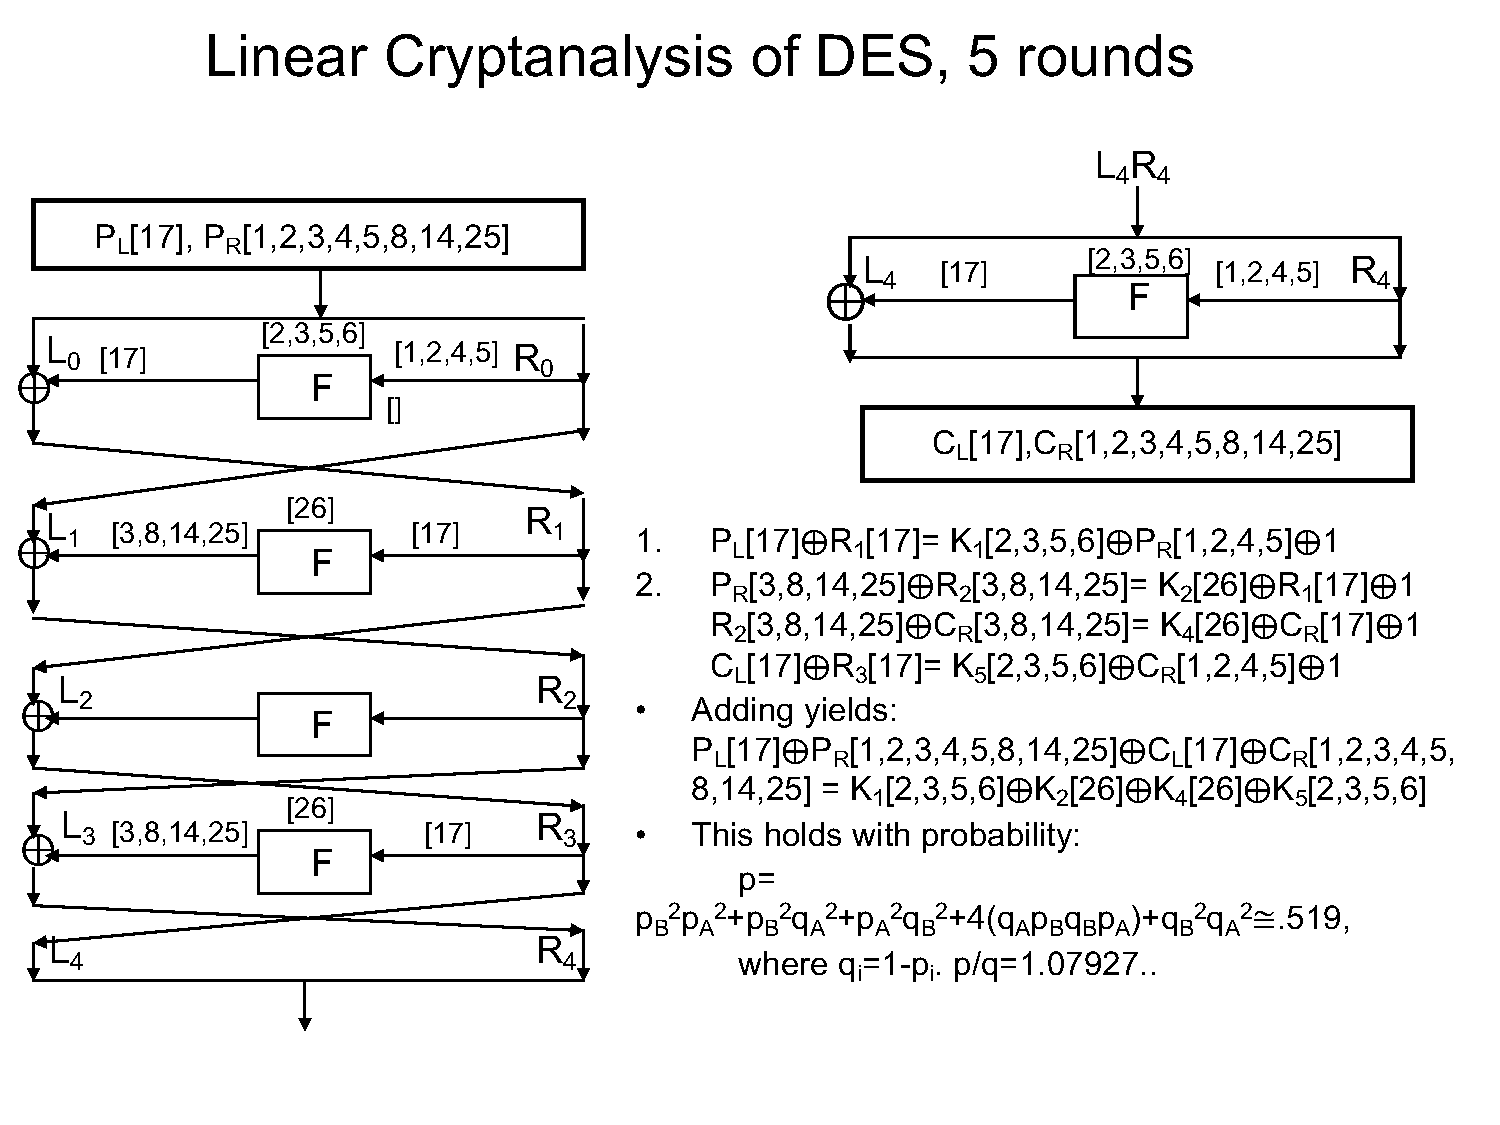
\includegraphics[width=0.8\textwidth,natwidth=642,natheight=610, height=80mm, width=88mm]{des.pdf}
\end{figure}
\\
{\bf Differential cryptanalysis: }  Notation: $ x \rightarrow y, p$ means
input difference $x$ produces output $y$ with probability $p$.
If $x' \rightarrow y'$ and $D_j(x',y')= \{u: S_j(u) \oplus S_j(u \oplus x')= y'\}$
then
$x \oplus k \in D_j(x', y')$, and $k \in D_j(x', y') \oplus x$.  Set
$\tau_j (x, x', y')= \{ k: k \in D_j(x',y') \oplus x \}$ and
$test_j (E_j , {E_j}^*, C_j ' ) = \tau_j(E_j, E_j \oplus E_j^{*}, C_j')$.
Note: some candidate keys will scritch.
To convert from chosen to known attack, select $2^{32} {\sqrt {2m}}$ pairs,
about $m$ of these will have the right difference 
$x$ produces output $y$ with probability $p$.
If $x' \rightarrow y'$ and $D_j(x',y')= \{u: S_j(u) \oplus S_j(u \oplus x')= y'\}$
then
$x \oplus k \in D_j(x', y')$, and $k \in D_j(x', y') \oplus x$.  Set
$\tau_j (x, x', y')= \{ k: k \in D_j(x',y') \oplus x \}$ and
$test_j (E_j , {E_j}^*, C_j ' ) = \tau_j(E_j, E_j \oplus E_j^{*}, C_j')$.
\\
\\
{\bf 3-round attack: } $(L_0 , R_0 )$, $R_3 = L_2 \oplus
f(R_2 , k_3 )= L_0 \oplus   f(R_0 , k_1 ) \oplus f(R_2 , k_3 )$.
Choose ${R_0}' = 000000$, so that
$f(R_0 , k_1 ) \oplus   f(R_0^* , k_1 ) = 0$, get
$R_3 '  = L_0 ' \oplus   f(R_2 , k_3 ) \oplus f(R_2^* , k_3 )$.
Set $C'= P^{-1} (R_3 ' \oplus L_0 ')$ which is the output xor for round 3.
Compute
$E=E(L_3 )$, $E^*=E(L_3^* )$.  Calculate
$test_j (E_j , {E_j}^*, C_j ' )$, for $j= 1,2,...,8$ after choosing
plaintexts.
Can do this since $R_2= L_3$ is known.
Note that key bits overlap on initial and final rounds and must satisfy both conditions.
\\
\\
{\bf Cost of differential cryptanalysis: }  The \emph{signal to noise ratio},
$S/N$ ratio,
is the ratio of the count in the correct key bin to the average count in a key bin.
For the differential attack to succeed, $S/N>1$.  Assume there are $m$ pairs of chosen text,
$p$ is probability of characteristic, $k$ is the number of key bins (number
of possible keys),
$\gamma$ is number of suggested keys per pair.  There are about $mp$ right pairs (and
the right key is always counted).  If
$\lambda$ is the ratio of non-discarded pairs to the number pairs, then the average
count is ${\frac {\gamma \lambda m} {k}}$ and so $S/N= {\frac {pk} {\gamma \lambda}}$.
Note that differential differs from the product of round differential characteristics (which
is what we used); the differential probability considers
all valid pairs with correct first and final round differentials combine (add) to provide
the differential probability estimate.  
Usually, however, the product of probabilities of the round characteristics
is a good estimate for the differential, if not, other attacks, like related
key attacks, often work.
\\
\\
{\bf 6-round attack:}  Use
$(L_0 ' , R_0 ')= (0x40080000, 0x04000000)$,
$(L_1 ' , R_1 ')= (0x04000000, 0x00000000)$, $p= .25$;
$(L_2 ' , R_2 ')= ( 0x00000000, 0x04000000)$, $p= 1$;
$(L_3 ' , R_3 ') = (0x04000000, 0x40080000)$, $p= .25$.
$L_6 = L_5 \oplus f(R_5, K_6 )$, $R_4 = L_3 \oplus f(R_3, K_4 )$, and $L_5= R_4$ so
$L_3 ' \oplus L_6 ' = f(R_3, K_4 ) \oplus f(R_5, K_6 ) \oplus f(R_3^*, K_4 ) \oplus f(R_5^*, K_6 )$.  
Estimate $L_3 ' = 0x04000000$ and $R_3 ' = 0x40080000$ with $p= {\frac 1 {16}}$.  
Use this to estimate input xor for S-boxes of round 4.  
Get $C_1 ' C_2 ' ... C_8 ' = P^{-1} (L_6 ' \oplus 0x04000000)$ and
$E_1 ' E_2 ' ... E_8 ' = E(R_5 )$.  
$f(K_6, R_5) \oplus f(K_6, R_5^*) = 0$ since xors to $S2, S5, S6, S7, S8 $ are $0$
so $f(K_4, R_3) \oplus f(K_4,R_3^*)= P^{-1} (L_6 ' \oplus 0x04000000)$.
Right pairs bump count for correct key bits, wrong pairs are random.  
\emph{Filter:}   If $|test_j (E_j , {E_j}^*, C_j ' )| = 0 $, for all  $j= 2,5,6,7,8$, this is a
wrong pair; the probability that a wrong pair satisfies this at random is 
$({\frac {4}{5}})^5 = {\frac 1 3}$ since only ${\frac 4 5}$ of the differentials are possible
in each S-box.  
${\frac 2 3}$ of the wrong pairs are detected this way, so
ratio of right pairs (``RP'') remaining is ${\frac {\frac 1 {16}} {{\frac 1 {16}} +
{\frac {15} {16}} \times {\frac 1 3}}}= {\frac 1 6}$.
Number of suggested pairs is
$\Pi |test_j (E_j , {E_j}^*, C_j ' )| $, for $j= 2,5,6,7,8$, correct values
will be suggested ${\frac {3n} {16}}$ times; incorrect strings at random
among approximately $2^{30}$ values.  Let $T_j$ be the counter vector of length 64.
For each pair compute $T^i_j$, $j= 2,5,6,7,8$, $1 \leq i \leq n$.  For
$I \subseteq \{ 1, 2, \ldots n \}$, $\sum_{i \in I} T^i_j$.  There
should be some $I$ of size about ${\frac {3n} {16}}$, this is the
suggested key.  Here $n$ is the number of pairs and
all of the remaining indexes have $1$ in the vector.
\\
\\
{\bf Another 3-round Characteristic:}
$L_0 ' , R_0 '$: 0x00200008, 0x00000400,
$L_1 ' , R_1 '$: 0x00000400, 0x00000000, $p= .25$;
$L_2 ' , R_2 '$: 0x00000000, 0x00000400, $p= 1$;
$L_3 ' , R_3 '$: 0x00000400, 0x00200008, $p= .25$.
{\bf Iterative Characteristic:} $\Omega_P= (19 60 00 00 | 00 00 00 00), p= {\frac 1 {234}}$.
These can be concatinated.
\\
\\
{\bf $5$-round differential and $0$R, $1$R, $2$R attacks:}
The differential is
$\Omega_P= (40 00 46 D0 || 02 00 00 00)= \Omega_T$ consisting of
$02 00 00 00 \rightarrow 40 00 40 10, p_1= {\frac {14} {64}}$,
$00 00 06 c0 \rightarrow 02 00 00 00, p_2= {\frac {12 \cdot 16} {64^2}}$,
$00 00 00 00 \rightarrow 00 00 00 00, p_3= 1$,
$00 00 06 c0 \rightarrow 02 00 00 00, p_2= {\frac {12 \cdot 16} {64^2}}$,
$02 00 00 00 \rightarrow 40 00 40 10, p_1= {\frac {14} {64}}$, with total
probability $p= {\frac 1 {9511}}$.  
In the \emph{$0$-R attack}, 
request ${\frac m p}$ pairs with $\Delta P= \Omega_P$.
Approximately $m$ pairs survive.  Given ``right pairs,'' $(P_1, P_2), (C_1, C_2)$,
we obtain $5$-bits of key from subkey $K_5$, using the active S-box, $S_2$, as follows.
Try all $2^5$ key candidates as a guess and calculate $S_2'$, if this is not
$7$ discard.  $14$ pairs survive.  Another right pair reduces this to $2$ after
$3-5$ right pairs, we're done.  A wrong pair satisfying $\Omega_P \rightarrow \Omega_T$
occurs with probability $2^{-64}$.  We can actually do the 
first and last rounds simultaneously to get $10$ key-bits.  To calculate $m$,
notice that we get about $2^{-64} {\frac m p}$ ``wrong pairs'' (``WP'') and the
total number of suggested wrong keys suggested is $2^{-54} {\frac m p}$ which is
negligible for $m < 2^{36}$.  Since there are $196$ subkeys suggested
$14^2$ values, ``right pair'' must agree on the $2$ shared bits, so
${\frac 1 4}$ of these survive this filter leaving $49$ subkeys on average.  The right
key is always among then.  A wrong key is suggested ${\frac {48} {1023}}m = .05m$ times.
If $t$ is the threshold for picking the key, 
$m= 2, t=2$ succeeds $.276$ of the time,
$m= 4, t=3$ succeeds $.53$ of the time and
$m= 5, t=3$ succeeds $.64$ of the time and
$m= 10, t=5$ succeeds $.91$ of the time.
In the \emph{$1$-R attack}, $f'= (40 00 46 D0)$ enters $F$ in sixth round and the pattern
$?0 00 ?? ??$ must emerge this gives a $32+12=44$ bit filter so given $40000$ pairs,
we expect $40000 \cdot 2^{-44} < 2^{-28}$ WP's to survive the filter.  Now examine the
input difference.
In the \emph{$2$-R attack}, request $100000$ pairs.  Output of $F$ in seventh round is
$C_L' \oplus (40 00 46 D0)$ and only $7$ bits after round $7$ are known.  All right pairs
suggest the correct key in round $7$.  We expect $33$ to suggest keys and $4^8$ subkeys
to be suggested per pair.  $33 \cdot 2^{16} \approx 2^{21}$ suggestions and wrong
keys are suggested ${\frac {2^{21}} {2^{48}}}= 2^{-27}$ times.
For linear \emph{$1$R}, guess subkey on last round and use distinguisher to confirm.
Ask for $N=c q^{-2}$ encryptions.
\\
\\
{\bf Linear cryptanalysis:} $\alpha \cdot P \oplus \beta \cdot C= \gamma \cdot C$ with
$p= {\frac {1} {2}} + \delta$ requires about $c \delta^{-2}$ plaintexts.
Last round estimation:
$L(P) \oplus M(C) \oplus N(P_{n-1} , K_n )= P(K)$ then use MLE: $T$= \# plain
cipher pairs $=0$ if 
$|T_{max} - {\frac {N} {2}}|>|{\frac {N} {2}} - T_{min}|$
and $p>.5$, guess $P(K)= 0$.
\\
\\
{\bf Basic Linear constraints in DES: }
\begin{center}
\begin{tabular} {|c|c|c|c|c|}
\hline
- & SBx & SBox Equation & Round Equation & Prob\\
\hline
A & $5$ & $X[2] \oplus Y[1,2,3,4]= K[2]\oplus1$ & $X[17] \oplus Y[3,8,14,25]= K[26] \oplus 1$ & ${\frac {52}{64}}$\\
B & $1$ & $X[1,4,5,6] \oplus Y[1,2,3]= K[1,4,5,6]\oplus1$ & $X[1,2,4,5] \oplus Y[3,8,14,25]= K[2,3,5,6] \oplus 1$ & ${\frac {42}{64}}$\\
C & $1$ & $X[2] \oplus Y[1,2,3,4]= K[2]\oplus1$ & $X[3] \oplus Y[17]= K[4] \oplus 1$ & ${\frac {34}{64}}$\\
D & $5$ & $X[2] \oplus Y[1,2,3]= K[2]\oplus1$ & $X[17] \oplus Y[8,14,25]= K[26]$ & ${\frac {42}{64}}$\\
E & $5$ & $X[1,5] \oplus Y[1,2,3]= K[1,5]\oplus1$ & $X[16,20] \oplus Y[8,14,25]= K[25,29] \oplus 1$ & ${\frac {48}{64}}$\\
\hline
\end{tabular}
\end{center}
Using round bit-numbering (and taking into account expansion and permutation),
the relation $S_5(x_1+k_1, x_2+k_2, x_3+k_3, x_4+k_4, x_5+k_5, x_6+k_6)+x_2= k_2$
becomes $X[17] \oplus Y[3,8,14,25]= K[26] \oplus 1$.
\\
\\
{\bf Best Differential attack on full DES: }
Use $0 \rightarrow 0$ together with $6$ concatenated $2$-round iterative differential 
characteristic with $p= {\frac 1 {234}}$ to obtain a $13$ round with $p= 2^{-47.2}$.
Use $2$R attack on last two rounds.  For first round, we want $19 60 00 00 || 00 00 00 00$
entering round $2$.  If we get $19 60 00 00$ to enter the $F$-function, the output
has $20$ $0$ bits and $12$ unknown bits. Chose plaintexts so that all possible
$2^{12}$-bit combinations occur in the $12$ bits on corresponding input plaintext.
Now choose $2^{35.2}$ such $12$ bit structures to insure $2^{47.2}$ pairs.  Analyze 
$2^{24}$ with difference $19 60 00 00$ in the right hand word yielding
$19 60 00 00 || 00 00 00 00$ after round $14$.  Candidate round $16$ pairs will have
$20$ ciphertext bits with $0$ difference.  Consider $2^{24} \cdot 2^{-20}$ of these.
An additional filter is used noting that $S_1$ with an input difference of $3$ can
only produce $15$ outputs and do the same for round $16$ leaving a survival ratio
of $0.0745$ or $1.19$ pairs from each of the $2^{35.2}$ structures.  Of the survivors,
analyze the output obtaining the key values for which it can be a ``right'' pair.
There are $52$ involved bits and $2^{52}$ key values.  Ratio of values that are not
discarded in round $16$ analysis is ${\frac {2^{-32}} {(.8)^8}}$.  
Probability that it
is not discarded in round $1$ or round $15$ analysis is ${\frac {2^{-12}} {
{\frac {13} {16}} \cdot
{\frac {14} {16}} \cdot
{\frac {15} {16}}}}$.  So a key has probability of $.84 \times 2^{-52}$ of being
suggested, yielding $1.19 \times .84 \approx 1$ key suggestion.  Now try
$2^4$ possible values for the remaining key to confirm.  There are actually two
such iterative differential characteristics reducing the complexity by a factor of
$2$.
\\
\\
{\bf Best Linear attack on full DES: }
Use the $14$ round approximation with bias $2^{-21.75}$ twice (once in reverse order).
The basic attack is:
(1) Ask for the encryption of $m$ random texts. (2) for each of the $24$ guessed bits
entering active S-Boxes in first and last round, partially encrypt and decrypt and
store values of pairs satisfying the approximation.  (3) Guess suggested key with maximal
deviation from ${\frac m 2}$.  This would normally involve a work factor of
$2^{43} \times 2^{24} \textnormal{ trial encryptions } \times 4 \textnormal{ S-boxes}
/ 128= 2^{62}$ but this is reduced to $2 \cdot (2^{43} \times 2^{12} \times 2 / 128= 2^{47}$
by doing each approximation seperately and doing the trial encryption once for each
of the $2^{12}$ possible S-box inputs.  
This gives $26$ bits $24 + 2 \textnormal{ from the approximation}$ 
with probability $.85$ and the other $30$ bits
are tried at random.
\\
\\
{\bf Note: } Suppose ${\vec f}: GF(2)^k \times GF(2)^n \rightarrow GF(2)^n$.
If ${\vec f}({\vec k}, {\vec x}_0)= (1,1, \ldots, 1)$ then
$g({\vec k}, {\vec x})= \prod_{i=1}^n f_i({\vec k}, {\vec x})$ is $0$ everywhere except
${\vec x}= {\vec x}_0$.
\\
\\
{\bf Basic Correlation matrix definitions: }
Let $f,g: GF(2)^n \rightarrow GF(2)$, define
$C(f,g)= 2 Prob[f(x)=g(x)] -1$, $\hat{f}(x) = (-1)^{f(x)}$,
$\langle \hat{f}, \hat{g} \rangle = \sum_x \hat{f}(x) \hat{g}(x) $,
$|| \hat{f}||= \sqrt{\langle \hat{f}, \hat{f} \rangle}$.  Note that
$C(f,g)= {\frac {\langle \hat{f}, \hat{g} \rangle} {||\hat{f}|| \cdot ||\hat{g}||}}$.
For $u \in GF(2)^n$ define $L_u(x)= u^T \cdot x$ then 
$\langle \hat{L}_u , \hat{L}_v \rangle= 2^n \delta (u \oplus v)$.
With this notation, the (normalized) \emph{Walsh transform} is
$F(w)= 2^{-n} \sum_x (-1)^{f(x) \oplus L_w(x)} = 
2^{-n} \langle \hat{f}, \hat{L}_w \rangle$.
Note that 
$\hat{f}(x)= \sum_w {\frac {\langle \hat{f}, \hat{L}_w \rangle} 
{||\hat{L}_w|| \cdot ||\hat{f}||}} \hat{L}_w(x)$ or
$\hat{f}(x)= \sum_w F(w) \hat{L}_w(x)$.  Denote ${\cal W}(f)= F$ and note that
$\sum_w F(w)^2 =1$.  If ${\cal BF}_n$ denotes the boolean functions from
$GF(2)^n$ to $GF(2)$,  we can define a map 
${\cal L}: {\cal BF}_n \rightarrow {\mathbb R}^{2^n}$ by $f \mapsto 
( (-1)^{f(0,\ldots, 0)},
(-1)^{f(0,\ldots, 1)}, \ldots,
(-1)^{f(1,\ldots, 1)})$.
If 
$f(x_1, \ldots, x_n) = (f_1(x_1, \ldots, x_n), f_2(x_1, \ldots, x_n), \ldots, 
f_m(x_1, \ldots, x_n)) $
then define the $m \times n$ \emph{correlation matrix} as $C^{(f)}= (c_{u,w}), 
c_{u,w}= C(u \cdot f(x), L_w)$.
\\
\\
{\bf Fast Hadamard Transform: }
$H_{2^m} = H_2 \otimes H_{2^{m-1}}$.
$H_{2^m}= M^{(1)}_{2^m} M^{(2)}_{2^m} \ldots M^{(m)}_{2^m}$,
$M^{(i)}_{2^m}= I_{2^{m-1}} \otimes H_2 \otimes I_{2^{i-1}}$.
\\
\\
{\bf Observation: }
A \emph{balanced boolean function} is uncorrelated with either constant function.
\emph{Question: } What is the best affine approximation of a balanced function?
The question is important because if $E(k,x)$ is a block cipher on blocks of $n$ bits, 
each $E_i(k,x)$ is a balanced boolean function.
How many inputs satisfy all approximations?  
For the correct input, what are the expected number of equations
that agree with it?  Variance, etc.
\\
\\
{\bf Theorem: }  $\sum_w F(w) = \pm 1$.
\begin{quote}
\emph{Proof: }
$\sum_w F(w)= \sum_w 2^{-n} \sum_x (-1)^{f(x)+ w \cdot x}
= 2^{-n} \sum_x (-1)^{f(x)} (\sum_w (-1)^{w \cdot x})=
2^{-n} \sum_x (-1)^{f(x)} 2^n \delta_{w,x}$, so
$\sum_x (-1)^{w \cdot x+c} =  (-1)^c , w =0, 0, w \ne 0$.
Let $F(w,c)= \sum_x (-1)^{f(x +  w \cdot x + c)}$
then $\sum_{w,c} F(w,c)= 0$.
\end{quote}
{\bf Theorem: }
If $h(x)= f(x) \oplus g(x)$ then $H(w)= \sum_v F(v \oplus w) G(v)$.
If $h(x)= f(x) \cdot g(x)$ then $\hat{h}(x)= {\frac 1 2} (1 + \hat{f}(x) + \hat{g}(x) -
\hat{f}(x) \cdot \hat{g}(x)
)$ and hence $H(w) = {\frac 1 2} (\delta(w) + 
{\cal W}(f) +
{\cal W}(g) -
{\cal W}(f \oplus g))$.  
\begin{quote}
\emph{Proof: }
Let $N= 2^n$.
$
\sum_u F(u)G(w+u)=
\sum_u
({\frac 1 N} \sum_s (-1)^{f(s)+s \cdot u})
({\frac 1 N} \sum_t (-1)^{g(t)+t \cdot (w+u)})=
\sum_u
({\frac 1 {N^2}} \sum_t (-1)^{f(s)} (-1)^{g(t)} (-1)^{t\cdot w} (-1)^{(s+t)\cdot u}) =
({\frac 1 {N^2}}) \sum_t (-1)^{f(s)} (-1)^{g(t)} (-1)^{t\cdot w} (\sum_u (-1)^{(s+t)\cdot u})$. 
The last sum is $0$ unless $s=t$ in which case it's $N$ so
$\sum_u F(u)G(w+u)= {\frac 1 N} \sum_t (-1)^{f(t)+g(t)+w \cdot t}$.
\end{quote}
{\bf Theorem: }
If $V= V_1 \oplus V_2$,
$f(u_1 + u_2)= f(u_1)$ and
$g(u_1 + u_2)= g(u_2)$ for $u_1 \in V_1, u_2 \in V_2$ and $h(x)= f(x) \oplus g(x)$ then
$H^{(V)}(u_1 + u_2)= F^{(V_1)}(u_1) G^{(V_2)}(u_2)$.  For example, $h(x, y)= (f(x), g(y))$,
$C^{(h)}=
\left(
\begin{array}{cccc}
1 & 0 & 0 & 0 \\
F(0) & F(1) & 0 & 0 \\
G(0) & 0 & G(1) & 0 \\
F(0)G(0) & F(1)G(0) & F(0)G(1) & F(1)G(1)\\
\end{array}
\right)
$.
\\
\\
{\bf Theorem: } If 
$C^{(f)}$ is invertible, $(C^{(f)})^{-1}= (C^{(f)})^{T}$.
\begin{quote}
\emph{Proof: }
If $h$ is invertible, $(C^{(h)})^{-1}= (C^{(h)})^T$.  For a bijection,
$C(u^T h^{-1}(a), w^Ta)= C(u^T b, w^T h(b))= C(w^T h(b), u^T b)^T$,
so, $C^{(h^{-1})}= (C^{(h)})^{-1}$.
\end{quote}
{\bf Theorem: }
$f$ is invertible iff $C^{(f)}$ is invertible.
\begin{quote}
\emph{Proof: }
The $\rightarrow$ direction follows from the inverse formula above.
The proof of $\leftarrow$: $(-1)^{u^T h(a)} = \sum_w C^{(h)}_{u,w} (-1)^{w^T a}$. 
If $C^{(h)}$ is invertible,
$(-1)^{w^T a} = \sum_u (C^{(h)})^{-1}_{w,u} (-1)^{u^T h(a)}$.  
If $\exists x \ne y: h(x) = h(y)$, substituting into
the equation above, $(-1)^{w^Tx}=(-1)^{w^Ty}$ and that is just wrong.
\end{quote}
{\bf Theorem: }
If $h(x)= f(g(x))$ then  $ C^{(h)}= C^{(f)} C^{(g)} $.
\begin{quote}
\emph{Proof: }
$(-1)^{u^T \cdot h(a)} =
\sum_v C^{(f)}_{u,v} (-1)^{v^T \cdot g(a)}=
\sum_v C^{(f)}_{u,v} ( \sum_w C^{(g)}_{v,w} (-1)^{w^T \cdot a})$.
\end{quote}
{\bf Theorem: }
If $h(x)= x \oplus a$ then $C^{(f)}_{u,u} = (-1)^{u^T \cdot a}$.
\begin{quote}
\emph{Proof: }
$u^T \cdot h(a)= u^T \cdot x \oplus u^T \cdot a$.
\end{quote}
{\bf Theorem: }
If $h(x)= Mx$ then $C^{(f)}_{u,w} = \delta(M^Tu \oplus w)$.
\begin{quote}
\emph{Proof:}
$u^T \cdot h(a)= (M^T u)^T a$.
\end{quote}
{\bf Theorem:}
$C_{u \oplus v, x} = \sum_w 
C_{u , w \oplus x} 
C_{v , w} $.
\begin{quote}
\emph{Proof:}
${\cal W}((u \oplus v)^T h(a)) = {\cal W}(u^T h(a)) \otimes {\cal W}(v^T h(a))$;
note that first transform on right is 
$C^{(h)}_{u,w}$ and second is
$C^{(h)}_{v,w}$.  One consequence is: $C_{u \oplus v, 0} = \sum_w C_{u,w} C_{v,w}$.
\end{quote}
{\bf Theorem:}  A Boolean transformation is invertible iff every output parity is
a balanced binary boolean function of the input bits. 
\begin{quote}
\emph{Proof:}  Let $C=C^{(h)}$.
$\rightarrow$: If $h$ is invertible, $C C^T = I$, $C_{00}=1$ and the norm of every
row and column is $1$.  $C(u^T h(a),0) = \delta(u)$; all rows except row $0$ are
correlated to $0$ hence the function is balanced for $u \ne 0$.
For $\leftarrow$: The condition on
output parities being balanced is $C_{u,0}=0, u \ne 0$. i.e.- $C$ is orthogonal.
$C C^T =I \leftrightarrow \sum_w C_{u,w} C_{v,w}= \delta(u \oplus v)$ (``*'') also
$\sum_w C_{u,w} C_{v,w} = C_{u \oplus v,0}$ but $C_{u,0}=0, u \ne 0$ and $C_{00}=1$
so ``*'' holds $\forall u,v$ hence $C$ is orthogonal and invertible so by the previous
result $h$ is invertible.  
\end{quote}
{\bf Theorem:} Let $u$ and $w$ are parities then and 
$F^u$ denotes the normalized Walsh transform of $u^T {\vec f}({\vec x})$ while
$G^w$ denotes the normalized Walsh transform of $w^T {\vec g}({\vec x})$ then
$(C({\vec f},{\vec g}))_{u,w}= \sum_v F^u(v) G^w(v)$.
\\
\\
{\bf Definition:} A \emph{linear trail} is 
$U= ( u_0, u_1, \ldots, u_r)$ associated with a composite function
$\beta= \rho_r \rho_{r-1} \ldots \rho_1$ with correlation contribution
at each step of $C((u_i^T \rho_i (a), u_{i-1}a)$ and overall 
correlation of $C_p(U)= \prod_i C^{\rho_i}_{u_{i}, u_{i-1}}$.
\\
\\
{\bf Theorem:}
$C(u^T \beta(a), w^T a)= \sum_{U, u^{(0)}=u, u^{(r)}=w} C_p(U)$.
\begin{quote}
\emph{Proof:}  Follows from definition.
\end{quote}
{\bf Theorem:} The correlation coefficients and spectrum values for a boolean function
over $GF(2)$ are integer multiples of $2^{1-n}$.  
\begin{quote}
\emph{Proof:}
The values are of the form
$k+(2^n-k)(-1)=2k-2^n$ which is even.
\end{quote}
{\bf Theorem:}
The correlation $\hat{c}_{fg}(b)= C(f(x), g(x \oplus b))= {\cal W}^{-1}(FG)$.
\begin{quote}
\emph{Proof:}
$\hat{c}_{fg}(b)= 2^{-n} \sum_a (-1)^{f(a) \oplus g(a \oplus b)} = C(f(x), g(x \oplus b))$.
\end{quote}
{\bf ``Bricklayer'' functions:} If 
$$h(a(1), \ldots,a(n))=
(h(1)(a(1), a(2), \ldots , a(n)), h(2)(a(1), a(2), \ldots , a(n)), \ldots,
h(n)(a(1), a(2), \ldots , a(n))),$$ then
$C^{(h)}_{uv}= \prod_{i=1}^n C^{h(i)}_{u_i,v_i}$.
\\
\\
{\bf Truncating Function:} Let $a'= \varphi^{v,\epsilon, s}(a)$ 
taking $\varphi: GF(2)^{n-1} \rightarrow GF(2)^{n}$ be
defined by  $a_i'=a_i$ for $i \ne s$ and $a_s'= \epsilon \oplus v^t a \oplus a_s$ 
where $v^Ta= \epsilon$ defined the restriction.  Then 
$C^{\varphi}_{w,w} =1$, 
$C^{\varphi}_{v \oplus w,w} = (-1)^{\epsilon}$, $\forall w: w_s= 0$; 
note there are two non-zero
entries both of amplitude 1.  
If $C'= C C^{\varphi}$,
$C'_{u,w}= C_{u,w} \oplus (-1)^{\epsilon} C_{u,v \oplus w}$ if $w_s=1$ and $0$ if
$w_s=0$.
\\
\\
{\bf Theorem:}
For \emph{key alternating ciphers}, $C_p(U)= \prod_i (-1)^{u_i^T k_i} C_{u_i, u_{i-1}}
= (-1)^{d_U \oplus \bigoplus_i u_{i}^T k_i }
|C_p(U)|$ where $d_U= 1$ if
$\prod_i (-1)^{u_i^T k_i} C_{u_i, u_{i-1}}<0$
and $0$ otherwise.
\\
\\
{\bf Theorem:}
$C(v^T \cdot \beta(a), w^Ta)=
\sum_{U, u_0=u, u_r=w} (-1)^{d_U \oplus U^TK} |C_p(U)|$.
\\
\\
Put $s_i= U^TK \oplus d_U$ and $C_i= C_p(U_i) (-1)^{s_i}$, then
averaging over the round keys, for all 
trail, we get:\\
\\
{\bf Theorem:}
$E(C_t^2)= 2^{-n_K} \sum_k ( \sum_i (-1)^{s_i} C_i)^2$.
\begin{quote}
\emph{Proof:}
$E(C_t^2)
= 2^{-n_K} \sum_k (\sum_i (-1)^{U_i^Tk \oplus d_{U_i} }C_i)^2
= 2^{-n_K} 
\sum_i \sum_j (\sum_k (-1)^{(U_i \oplus U_j)^Tk \oplus d_{U_i} \oplus d_{U_j}}C_i C_j)$.
But $C_i C_j = 2^{n_K} \delta(i \oplus j)$.
\end{quote}
For key schedule $K=M_{\kappa}(k)$, $E(C_t^2)= 2^{-n_K} \sum_i \sum_j ( \sum_k
(-1)^{(d_{U_i} \oplus d_{U_j})^T M_{\kappa}k \oplus d_{U_i} \oplus d_{U_j}})C_i C_j$.
The inner sum simplifies to 
$(-1)^{d_{U_i} \oplus d_{U_j}}2^{n_K} \delta(M_{\kappa}^T(U_i \oplus U_j))$.
If key schedule is not linear $K=f_{\kappa}(k)$, the coefficient of the mixed
term is $(-1)^{(U_i \oplus U_j)^T f_{\kappa}(k) \oplus d_{U_i} \oplus d_{U_j}}$.
\\
\\
{\bf Observation:}
Multiround linear expressions correspond to
linear trails.
Generally, $|C_p(U)|$ is independent of round key but this is not the case in DES because
of the shared bits between S-boxes.  $32$ bit input parities before $E$ give rise to $\alpha$
$2^{2l}$-$48$ bit patterns.  If $l$ is the number of pairwise neighboring S-boxes,
we can do this in $16l$ multiplications and additions.
The probability that a multiround expression holds 
is ${\frac 1 2}(1+C_p(U))$ for the associated
trail.
\\
\\
{\bf Observation:}
All Hadamard transform values of
\emph{bent functions} are equal to
$\pm 2^{\frac m 2}$ and hence the distance to any affine function is
$2^m \pm 2^{{\frac m 2} -1}$.  If $f(x_1, x_2,\ldots,x_m)$ is bent and $m \ge 6$ then
$f$ is indecomposable.  
$f(u_1, \ldots, u_m, v_1, \ldots, v_m) = 
g(v_1, \ldots , v_m) + \sum_i u_i v_i$ is bent.
If $f(u_1, \ldots, u_m, v_1, \ldots, v_m) = \sum_i u_i v_i$, then
$f+u_1 u_2, u_3$, $f+u_1 u_2, u_3 u_4$, \ldots,
$f+u_1 u_2, u_3 \ldots u_m$ are all inequivalent bent functions.\\
\\
{\bf Correlation Immunity:}
In this paragraph, $F$ denotes the unnormalized Walsh transform of $f$.  A function
$z=f(x_1 , \ldots , x_n)$ on $n$ variables 
$x_1, \ldots, x_n$ is $m$-th order \emph{correlation immune} if for every subset of these
variables or size $m$, $I(z; x_{i_1}, \ldots, x_{i_m})=0$.  If
$f$ has correlation immunity $m$ and non-linear order $k$, $m+k \le n$.  Let 
$N_{ab}(\omega)= | \{ x: z=f(x)=a, \omega \cdot x = b \} |$ then
$F(\omega)= N_{10}(\omega) - N_{11}(\omega)$.  Denote $p_a = P(z=a)$ then
$P(\omega \cdot x = b | z=a)=
{\frac {P(\omega \cdot x=b, z=a)} {P(z=a)}}=p_a^{-1}2^{-n} N_{ab}(\omega)$.  We obtain the
following:
$P(\omega \cdot x=0 | z=1)= {\frac 1 2} + p_1^{-1} 2^{-n-1} F(\omega)$,
$P(\omega \cdot x=1 | z=1)= {\frac 1 2} - p_1^{-1} 2^{-n-1} F(\omega)$,
$P(\omega \cdot x=0 | z=0)= {\frac 1 2} + p_0^{-1} 2^{-n-1} F(\omega)$,
$P(\omega \cdot x=1 | z=0)= {\frac 1 2} - p_0^{-1} 2^{-n-1} F(\omega)$.
Let $h(t)= - t lg(t) - (1-t) lg(1-t)$.  
\\
{\bf Theorem 1:}  Let $x_0, \ldots, x_{n-1}$ be
independent and uniformly distributed arguments of the boolean function $f$ whose output
is the random variable $z$; then $\forall \omega \ne 0,
I(z; \omega \cdot x)= 1 - p_0 h({\frac 1 2} - {\frac {F(\omega)} {2^{n+1} p_0}})
- p_1 h({\frac 1 2} - {\frac {F(\omega)} {2^{n+1} p_1}})$.  
Moreover, when $z$ is uniformly distributed then
$I(z; \omega \cdot x)= 1 - h({\frac 1 2} - 2^{-n} F(\omega))$.
$F$ thus describes
the best affine approximation of $f$ (pick $\omega$ with largest coefficient, the
coefficients of the best affine approximation has coefficients of 1 for the corresponding
variables).  This generalizes to
\\
{\bf Theorem 2:}  Let $x_0, \ldots, x_{n-1}$ be
independent and uniformly distributed arguments of the boolean function $f_i \in {\cal F}$ 
where ${\cal F} = \{ f_1 , \ldots , f_m \}$, $p_f= {\frac 1 m}$ and the 
outputs of the randomly selected $f_i$ is the random variable $z$; then $\forall \omega \ne 0,
I(z; \omega \cdot x)= 1 - p_0 h({\frac 1 2} - {\frac {\sum_{i=1}^m F_i(\omega)} {2^{n+1} m p_0}})
- p_1 h({\frac 1 2} - {\frac {\sum_{i=1}^m F(\omega)} {2^{n+1} m p_1}})$.  
Moreover, when $z$ is uniformly distributed then
$I(z; \omega \cdot x)= 1 - h({\frac 1 2} - 2^{-n+1} m^{-1} \sum_{i=1}^m F_i(\omega))$.
Again, this provides the best affine approximation for the set of functions.  Finally,
this implies {\bf Theorem 3:} A boolean function $f$ is correlation immune of order $m$
if $F(\omega)=0, \forall \omega: 1 \le wt(\omega) \le m$. \\
\\
{\bf Counting Results:} Let $N=2^n$ and $BF(n)$ denotes the set of boolean functions on $n$-bit
values then $|BF(n)|= 2^N$. Let $BBF(n)$ be the balanced functions on $n$ bits then
$|BBF(n)|= {N \choose {\frac N 2}}$, $|GA(n)| \approx 2^{m^2+m}$.\\
\\
{\bf The natural isomorphism:}
${\cal L}: GF(2)^n \rightarrow {\mathbb R}^{2^n}$ by $a \mapsto (-1)^{a^T \cdot x}$.
${\cal L}(a+b)= {\cal L}(a) {\cal L}(b)$ by pointwise multiplication.  
Almost directly from the definitions, we get {\bf Theorem:}
$C^{(h)}({\cal L}(a))= {\cal L}(h(a))$.  
\\
\\
{\bf Theorem:} The elements of a correlation matrix corresponds to an invertible
transform of $n$-bit vectors are integer multiples of $2^{2-n}$.  The proof uses
the restriction map and the fact that $\sum (F(w) + F(w+v))^2 = 2$.
\\
\\
{\bf Theorem:} 
Let $F_q, q=2^n$, $Tr_{F_q/F_2}(x)=Tr(x)= \sum_{i=0}^{n-1} x^{2^i}$.
$Tr(x) \ne 0$ for some $x$.
$Tr(x+y)= Tr(x)+Tr(y)$.
$Tr(x^2)= Tr(x)$.
$Tr(x) \in F_2$.
$Tr(\omega x)$ is linear in $x$.
$Tr(\omega_1 x)= Tr(\omega_2 x) \rightarrow \omega_1 = \omega_2$.
$Tr(\omega x)$ are exactly the linear functions.
\\
\\
{\bf Definition:}
$F: F_{2^n} \rightarrow F_{2^m}$ is \emph{differentially $\delta$ uniform} if
$\forall \alpha, \beta, \alpha \ne 0$: $|\{ x: F(x+\alpha)+F(x)= \beta \}| \leq \delta$.
{\bf Theorem:} $F(x)= x^{2^k + 1}$, $s=(k,n)$ then $F$ is differentially $2^s$-uniform.
$N(F)= 2^{n-1} - 2^{{\frac {n+s} 2} -1}$.
{\bf Theorem:}  Let $G(x)= x^{-1}, x \ne 0; 0, x=0$.  $F$ is differentially 4 uniform.
$N(G) \geq 2^{n-1}-2^{{\frac n 2}}$.
\\
\\
{\bf Boolean functions:}
$a \vee b = a \oplus b \oplus ab$ as a boolean function.  Let ${\vec x}= (x_4 , x_3, x_2, x_1)$
with $x_1$ the least significant bit.
${\vec F} ({\vec x})=
(F_4 ({\vec x}), F_3 ({\vec x}), F_2 ({\vec x}), F_1 ({\vec x}))$.
If $\rho= (0000, 0001)$ then 
${\vec {F_i^{\rho}}}({\vec x})= x_i, i>1$ and 
${\vec {F_1^{\rho}}}({\vec x})= 
({\overline {x_2 \vee  x_3 \vee x_4}}) (x_1 \oplus 1) \oplus
(x_2 \vee x_3 \vee x_4) x_1= 1 \oplus x_1 \oplus x_2 \oplus x_3 \oplus x_4
\oplus x_2 x_3 \oplus x_2 x_4 \oplus x_3 x_4 \oplus x_2 x_3 x_4$.  If
$\sigma = (0000, 0001, \ldots , 1111)$, then
${\vec {F_1^{\sigma}}} ({\vec x})= x_1 \oplus 1$,
${\vec {F_2^{\sigma}}} ({\vec x})= x_1 (x_2 \oplus 1) \oplus {\overline {x_1}}x_2
= x_1 \oplus x_2$,
${\vec {F_3^{\sigma}}} ({\vec x})= (x_1 x_2) (x_3 \oplus 1) \oplus ({\overline {x_1 x_2}})x_3
= x_1 x_2 \oplus x_3$,
${\vec {F_4^{\sigma}}} ({\vec x})= (x_1 x_2 x_3 ) (x_4 \oplus 1) \oplus 
({\overline {x_1 x_2 x_3}}) x_4= x_1 x_2 x_3 \oplus x_4$.\\
\\
{\bf Theorem:} $RM(r,m)$ has minimum distance $2^{m-r}$.
$R(1,5)$ has $48$ inequivalent affine classes.
\\
\\
{\bf Balence:}
Each possible Boolean transformation on $n$ bits is a permutaion on the $2^n, n$-bit values
and so listing them in order, the columns are the possible ${\vec f}$ vectors representing the 
component functions.  If we label these as points in $GF(2)^{2^n}$ and draw an edge between
allowable co-components with the edges labeled by the correlation between these vectors,
any allowable $n$ boolean functions form a complete graph with the label $0$ on each edge.
$C(f,g)= 1-{\frac {wt(f+g)} {2^{n-1}}}$.  
{\bf Generalized Balence Theorem:} For each $n \le 128$ and each
$1 \le b_1 < b_2 < \ldots < b_n \le 128$ and fixed ${\vec k}$,
$(E_{b_1} ({\vec k}, {\vec x}), E_{b_2} ({\vec k}, {\vec x}), 
\ldots , E_{b_n} ({\vec k}, {\vec x}))$
takes each value in ${\mathbb Z}_2^n$ as ${\vec x}$ varies over
${\mathbb Z}_2^n$.  So does any non-trivial sum of any of these functions.
{\bf Theorem:}  If $f:GF(2)^{n-1} \rightarrow GF(2)$ is any boolean function,
$g(x_1, \ldots, x_n)= f(x_1, \ldots, x_{n-1})+x_n$ is balanced.
\\
\\
{\bf Advantage:}
Write $\epsilon= E_K$ and $\epsilon'= E_{K'}$.  What does $[\epsilon^i, {\epsilon'}^j]$ reveal
about $K$ for known $K'$.  Let ${\cal P}= \{ p_1 , p_2 , \ldots , p_m \}$ and let $l$ be given
put $N= p_1^l \ldots p_m^l$ and denote the set of $n$-bit elements of the block by
$S$;  what is ${\mathbb C}_S(\epsilon^N)$?  
How do you characterize the $x: g(x)=x$ where, say, $g$ represents $N$ applications of
$\epsilon$.  
In general, $\epsilon$ is complicated but
$\epsilon^m=1$ for some $m$ and
$\epsilon^t$ many be much simpler for some $m<t$.
Let $ g^{(0)}_{(i)}(x_1 , x_2 , \ldots , x_{i-1},x_{i+1}, \ldots, x_n)=
f(x_1 , x_2 , \ldots , x_{i-1},0,x_{i+1}, \ldots, x_n)$.  
{\bf Idea:} Suppose 
$\epsilon^i$ and $\epsilon^j$ are relatively easy to determine 
(low degree, good approximation whatever)
and $(i,j)=1$ then we can find $a, b: ai+bj=1$ and calculate
$\epsilon= (\epsilon^i)^a (\epsilon^j)^b= \epsilon$.  Let $B_n(r,{\vec v})=
\{ {\vec x} :  wt({\vec v} \oplus {\vec x}) =r \}$. $|B_n({\vec v}, r)|= 2^{n-r}$.  
Motivation for idea is while
there are lots of ``far away'' approximations of $\epsilon$ there aren't many near ones.  
However,
there may be close approximations of $\epsilon^i$.
\\
\\
{\bf Theorem:}
Let $f$ be the Boolean function defined by
$S^0_f= \{x: f(x)=0 \}$ and
$S^1_f= \{x: f(x)=1 \}$.  
If $e_i(x)= E_i(k,x)$ then 
$| S^{b}_{e_1} \cap S^{b}_{e_2} \cap \ldots \cap S^{b}_{e_k} |=2^{n-k}$.  What
are the permutations that fix such a set?
\\
\\
{\bf Theorem:}
Let $f,g: GF(2)^n \rightarrow GF(2)$ and $N= 2^n$.
Let $a$ be the number of positions where $f$ and $g$ agree and
$d$ be the number of positions where $f$ and $g$ disagree, then
$Pr[(f(x)=g(x)] = {\frac a {2^n}}$.
Note that
$wt(f \oplus g)=d= dist(f,g)$.  
Now suppose $g(x)= w \cdot x$,
the linear function.  $F(w)= {\frac 1 {2^n}} \sum_x (-1)^{f(x)=g(x)}= {\frac 1 {2^n}} (a-d)$
Since $a+d=2^n$, $F(w)= 2 {\frac a {2^n}} -1$ and thus $C(f,w)= F(w)$.  These yield
$dist(f(x),w \cdot x)= 2^n(1-F(w))$.  Thus the best affine approximation is the one which
maximizes $|F(w)|$ for some $w$.
\\
\\
{\bf Theorem:}
Now let $f: GF(2)^n \rightarrow GF(2)$ be a bijective boolean transformation with component
functions $f_1 , f_2 , \ldots , f_n$.  All such transformations represent
permutations in $S_{2^N}$ and the correlation matrices of these transformations is orthogonal
($C C^T = I$).  A block cipher gives rise to such transformations by setting $f(x)= E_K(x)$ for
fixed $K$.  Note that all balanced boolean functions can be obtained by applying a
permutation in $S_{2^N}$ to a sequence of ${\frac N 2}$, $1$'s and ${\frac N 2}$, $0$'s.
\\
\\
{\bf Theorem 1:} 
With the foregoing notation,
$C(f_i,1)= C(f_i,0)=0$, $C(f_i, f_j)=0, i \ne j$,
$wt(f_i)= 2^{n-1}, \forall i$, $wt(f_i f_j) = 2^{n-2}, i \ne j$ and in general,
$wt( f_{i_1} f_{i_2} \ldots f_{i_k})= 2^{n-k}$.  Further, $C(f_i f_j, f_k)= {\frac 1 2}$ ,
$C(f_i, f_j, f_k f_l) = C(f_i f_j f_k, f_l)$ and
in general
$C( f_{i_1} f_{i_2} \ldots f_{i_k}, f_l)= 2^{n-k-1}$. Let $f$ be a boolean function.
{\bf Theorem 2:}  Let $f$ be a boolean function.  The $N$ functions
$f_{i_1} f_{i_2} \ldots f_{i_k}$ form a basis for the space of boolean functions; that is,
for any boolean function $g$,
$\exists a^{(g)}_{i_1, i_2, \ldots, i_k}$ such that $g(x)= \sum_{1\le i_1 < i_2< \ldots < i_k = n}
a^{(g)}_{i_1, i_2, \ldots, i_k}
f_{i_1} f_{i_2} \ldots f_{i_k}$.  In particular, there are such coefficients such that
$x_i= \sum_{1\le i_1 < i_2< \ldots < i_k = n}
a^{(x_i)}_{i_1, i_2, \ldots, i_k} f_{i_1} f_{i_2} \ldots f_{i_k}$.  Define
$Appx_i(f)= \{ g: dist(f,g) \le i \}$, then $|Appx_i(f)|= \sum_{j=0}^i{N \choose i}$.
\\
\\
$NL(f) \le 2^{n-1}- 2^{{\frac n 2} -1}$,  $NL(f) \le 2^{n-1} +
{\sqrt {2^n + max_{e \ne 0} (F(D_e(f)))}}$, where $D_e f = f(x) \oplus f(x \oplus e)$.
\\
\\
{\bf Theorem (Rothaus):} Let $n \ge 4$ of even algebraic degree then any bent function
on $GF(2)^n$ has degree $\le {\frac n 2}$. An $n$-Boolean function, $f$, is $m$-resilient
iff $f$ is balanced and $F(u)=0, \forall u: wt(u) \le m$.  
Maiorana-MacFarland class ${\cal M}= \{f: f(x,y)=x \pi(y) \oplus g(y) \}$ where $\pi$ is
a permutation on $GF(2)^{\frac n 2}$ and $g$ is affine.  
$|{\cal M}|= (2^{\frac n 2})! 2^{\frac n 2}$.   
For \emph{bent quadratics}, $\bigoplus_{1 \le i,j \le n}
a_{ij} x_i x_j \oplus h(x)$, $h$, affine.
\\
\\
{\bf Definition:}
For this section, $f:GF(2)^m \rightarrow GF(2)$.  The \emph{sensitivity} of $v$
is defined by $S(v) = | \{ v': f(v) \ne f(v'), dist(v,v') = 1 \}|$.  The average sensitivity
$aS(f)= {\frac 1 {2^m}} \sum_v S(v)$.  The \emph{influence} of $x_i$
is defined by
$I(x_i)= Prob(f(x_1,\ldots,x_{i-1},y,x_{i+1},\ldots, x_m)$, the probability
that the function is determined no matter what $y$ is.
\\
\\
{\bf Theorem:}  Let $f$ be a boolean function of $n$ variables with average
sensitivity $aS(f)=k$.  Let $\epsilon > 0$ and $M={\frac k {\epsilon}}$ then
(1) $\exists h$ depending on 
$exp((2+{\sqrt {\frac {2 log(4M)} M}})M)$ variables
such that $Prob(f \ne h) \le \epsilon$; and,
(2) $\exists g$ of degree at most
$exp((2+{\sqrt {\frac {2 log(4M)} M}})M)$ such that $Prob(f \ne g) \le {\frac {\epsilon} 2}$.
\\
\\
{\bf Basic Question:}
Let $F$ be a family of $m$ binary $n$-vectors.  How densely packed is $F$?
Given $b \le n$, $|F|$, what is the largest possible number of pairs of vectors
in $F$ whose Hamming distance is less than $b$?
\\
\\
{\bf Trace and correlation in $GF(2^n)$:}
$C^f_{u,w}= 2^{-n} \sum_a  (-1)^{Tr(wa)} (-1)^{Tr(u f(a))}$ so the terms are
determined by the condition $Tr(wa+uf(a))=0$, if this is satisfied by $r$ values
the entry is $r 2^{1-n}$.  If a function is linear over $GF(2^n)$, it is linear
over $GF(2)$ but not vice versa.
\\
\\
{\bf Theorem:}
Let $r_n$ be the ratio of the number of invertible $n \times n$ matrices over
$GF(2)$ to the number of $n \times n$ matrices over $GF(2)$, then
$lim_{n \rightarrow \infty} (r_n) \approx 0.288$.
\begin{quote}
\emph{Proof:}
The number of invertible $n \times n$ boolean matrices is
$t_n= (2^n-1) (2^n-2) \ldots (2^n-2^{n-1})$.  
The number of $n \times n$ boolean matrices is $2^{n^2}$.
$t_n= 2^{\frac {n(n-1)} 2} (2^n-1)(2^{n-1}-1) \ldots (2-1)$. 
Define $s_n= (2^n-1)(2^{n-1}-1) \ldots (2-1)$.
Now 
$t_{n+1}= 
2^{\frac {n(n+1)} 2} s_{n+1}= 
2^{\frac {n(n+1)} 2} 2^{-{\frac {n(n-1)} 2}} (2^{\frac {n(n-1)} 2} s_{n}) (2^{n+1}-1)= 
2^n (2^{n+1}-1) t_{n}$.  
Dividing both sides of this by $2^{(n+1)^2}$, we get
$r_{n+1}= {\frac {t_{n+1}} {2^{(n+1)^2}}}= 
{\frac {2^n} {2^{2n+1}}} 
{\frac {t_{n} } {2^{n^2}}} (2^{n+1}-1) = r_n (1- 2^{-(n+1}))$.  
Using this recurrence, we get $r_n= \prod_{i=1}^n (1-2^{-n})$.
The product approaches $\approx 0.288$ as $n \rightarrow \infty$.
\end{quote}
{\bf Question:}  Is there an easy to compute function, $T_K$, obviously non-linear,
so that $T_K E_K T_K^{-1}$ has good linear approximations?
How do you find such $T_K$?
Finding the best approximation reduces to finding an orthogonal transformation that
maximizes the largest entry.  Suppose $T$ is such a matrix; if $T$ has all bad affine approximations
is it possible that there is another orthogonal transformation, $R$ with
$T^R= R^{-1} T R$
such that $max_{ij}(|(T^R)_{ij}|)> max_{ij}(|(T)_{ij}|)$? If 
$\rho_1 , \rho_2 , \ldots , \rho_n$ is a series of such transformations (like the iterated
components of a block cipher), note that $R^{-1} E_K(x) R= 
R^{-1} \rho_1 R
R^{-1} \rho_2 R \ldots
R^{-1} \rho_n R$ thus raising the possibility of better ``per round'' approximations on a
related cipher.
\\
\\
Here is a motivating example
in ${\mathbb R}^3$:
$R=
\left(
\begin{array}{ccc}
cos(\varphi) & sin(\varphi) & 0\\
-sin(\varphi) & cos(\varphi) & 0\\
0 & 0 & 1\\
\end{array}
\right)$,
$T=
\left(
\begin{array}{ccc}
1 & 0 & 0\\
0 & cos(\theta) & sin(\theta)\\
0 & -sin(\theta) & cos(\theta)\\
\end{array}
\right)$ and
$$R^{-1}TR=
\left(
\begin{array}{ccc}
cos^2(\varphi)+cos(\theta)sin^2(\varphi) & 
cos(\varphi) sin(\varphi) - cos(\theta)cos(\varphi) sin(\varphi) & 
-sin(\varphi)sin(\theta)\\
-cos(\varphi) sin(\varphi) + cos(\theta)cos(\varphi) sin(\varphi) & 
sin^2(\varphi)+cos(\theta)cos^2(\varphi) & 
sin(\varphi)sin(\theta)\\
sin(\varphi)sin(\theta) &
-cos(\varphi)sin(\theta) &
cos(\theta) \\
\end{array}
\right)$$
\\
\\
$NL(f) \le 2^{n-1}- 2^{{\frac n 2} -1}$,  $NL(f) \le 2^{n-1} +
{\sqrt {2^n + max_{e \ne 0} (F(D_e(f)))}}$, where $D_e f = f(x) \oplus f(x \oplus e)$.
\\
\\
{\bf Prolog to computing DES correlation matrix:}  Let
$f(x_1, x_2, x_3, x_4)= ( x_1 + f_1(x_3 , x_4) , x_2 + f_2(x_3 , x_4) , x_3, x_4)$ (first
position most significant) then, with least significant positions indexing rows and columns, and
$F_i(w)$ as the Walsh transform for
$f_i(x_3 , x_4)$ and $H(w)$ the Walsh transform of $h(x)= f_1(x)+f_2(x)$.  Bit positions
in this example are $(x_1, x_2 , x_3 , x_4 )$.
$$C^{(f)}=
\left(
\begin{array}{cccc|cccc|cccc|cccc}
1 & 0 & 0 & 0 & 0 & 0 & 0 & 0 & 0 & 0 & 0 & 0 & 0 & 0 & 0 & 0 \\
0 & 1 & 0 & 0 & 0 & 0 & 0 & 0 & 0 & 0 & 0 & 0 & 0 & 0 & 0 & 0 \\
0 & 0 & 1 & 0 & 0 & 0 & 0 & 0 & 0 & 0 & 0 & 0 & 0 & 0 & 0 & 0 \\
0 & 0 & 0 & 1 & 0 & 0 & 0 & 0 & 0 & 0 & 0 & 0 & 0 & 0 & 0 & 0 \\
\hline
0 & 0 & 0 & 0 &  F_2(0) &  F_2(1) &  F_2(2) &  F_2(3) & 0 & 0 & 0 & 0 & 0 & 0 & 0 & 0 \\
0 & 0 & 0 & 0 &  F_2(1) &  F_2(0) &  F_2(3) &  F_2(2) & 0 & 0 & 0 & 0 & 0 & 0 & 0 & 0 \\
0 & 0 & 0 & 0 &  F_2(2) &  F_2(3) &  F_2(0) &  F_2(1) & 0 & 0 & 0 & 0 & 0 & 0 & 0 & 0 \\
0 & 0 & 0 & 0 &  F_2(3) &  F_2(2) &  F_2(1) &  F_2(0) & 0 & 0 & 0 & 0 & 0 & 0 & 0 & 0 \\
\hline
0 & 0 & 0 & 0 & 0 & 0 & 0 & 0 &  F_1(0) &  F_1(1) &  F_1(2) &  F_1(3) & 0 & 0 & 0 & 0 \\
0 & 0 & 0 & 0 & 0 & 0 & 0 & 0 &  F_1(1) &  F_1(0) &  F_1(3) &  F_1(2) & 0 & 0 & 0 & 0 \\
0 & 0 & 0 & 0 & 0 & 0 & 0 & 0 &  F_1(2) &  F_1(3) &  F_1(0) &  F_1(1) & 0 & 0 & 0 & 0 \\
0 & 0 & 0 & 0 & 0 & 0 & 0 & 0 &  F_1(3) &  F_1(2) &  F_1(1) &  F_1(0) & 0 & 0 & 0 & 0 \\
\hline
0 & 0 & 0 & 0 & 0 & 0 & 0 & 0 & 0 & 0 & 0 & 0 &  H(0) &  H(1) &  H(2) &  H(3) \\
0 & 0 & 0 & 0 & 0 & 0 & 0 & 0 & 0 & 0 & 0 & 0 &  H(1) &  H(0) &  H(3) &  H(2) \\
0 & 0 & 0 & 0 & 0 & 0 & 0 & 0 & 0 & 0 & 0 & 0 &  H(2) &  H(3) &  H(0) &  H(1) \\
0 & 0 & 0 & 0 & 0 & 0 & 0 & 0 & 0 & 0 & 0 & 0 &  H(3) &  H(2) &  H(1) &  H(0) \\
\end{array}
\right)$$
{\bf Feistel:}
A typical round of DES consists of two involutions: $\tau$ and $\sigma_k$.
$\sigma_k (L,R)= (L \oplus f(R,k), R)$, $f(x,k)= P S_1 S_2 \ldots S_8 (E(x)+k))$.
$\tau(L,R)= (R,L)$.
First ``line'' of $\sigma_k$ is 
$y_9= x_9 \oplus S_1^1(x_{64}+k_1,x_{33}+k_2,x_{34}+k_2, x_{35}+k_2, x_{36}+k_2, x_{37}+k_2)$,
$y_{17}= 
x_{17} \oplus S_1^2(x_{64}+k_1,x_{33}+k_2,x_{34}+k_2,x_{35}+k_2, x_{36}+k_2, x_{37}+k_2)$,
$y_{23}= 
x_{23} \oplus S_1^3(x_{64}+k_1,x_{33}+k_2,x_{34}+k_2,x_{35}+k_2, x_{36}+k_2, x_{37}+k_2)$,
$y_{31}=
x_{31} \oplus S_1^4(x_{64}+k_1,x_{33}+k_2,x_{34}+k_2, x_{35}+k_2, x_{36}+k_2, x_{37}+k_2)$.
\\
\\
Suppose $\tau (x_1, x_2, x_3, x_4)= (x_3, x_4, x_1, x_2)$, with position $(0001)$ representing
$x_4$, then
$$C^{(\tau)}=
\left(
\begin{array}{cccccccc|cccccccc}
1 & 0 & 0 & 0 & 0 & 0 & 0 & 0 & 0 & 0 & 0 & 0 & 0 & 0 & 0 & 0\\
0 & 0 & 0 & 0 & 1 & 0 & 0 & 0 & 0 & 0 & 0 & 0 & 0 & 0 & 0 & 0\\
0 & 0 & 0 & 0 & 0 & 0 & 0 & 0 & 1 & 0 & 0 & 0 & 0 & 0 & 0 & 0\\
0 & 0 & 0 & 0 & 0 & 0 & 0 & 0 & 0 & 0 & 0 & 0 & 1 & 0 & 0 & 0\\
0 & 1 & 0 & 0 & 0 & 0 & 0 & 0 & 0 & 0 & 0 & 0 & 0 & 0 & 0 & 0\\
0 & 0 & 0 & 0 & 0 & 1 & 0 & 0 & 0 & 0 & 0 & 0 & 0 & 0 & 0 & 0\\
0 & 0 & 0 & 0 & 0 & 0 & 0 & 0 & 0 & 1 & 0 & 0 & 0 & 0 & 0 & 0\\
0 & 0 & 0 & 0 & 0 & 0 & 0 & 0 & 0 & 0 & 0 & 0 & 0 & 1 & 0 & 0\\
0 & 0 & 1 & 0 & 0 & 0 & 0 & 0 & 0 & 0 & 0 & 0 & 0 & 0 & 0 & 0\\
0 & 0 & 0 & 0 & 0 & 0 & 1 & 0 & 0 & 0 & 0 & 0 & 0 & 0 & 0 & 0\\
0 & 0 & 0 & 0 & 0 & 0 & 0 & 0 & 0 & 0 & 1 & 0 & 0 & 0 & 0 & 0\\
0 & 0 & 0 & 0 & 0 & 0 & 0 & 0 & 0 & 0 & 0 & 0 & 0 & 0 & 1 & 0\\
0 & 0 & 0 & 1 & 0 & 0 & 0 & 0 & 0 & 0 & 0 & 0 & 0 & 0 & 0 & 0\\
0 & 0 & 0 & 0 & 0 & 0 & 0 & 1 & 0 & 0 & 0 & 0 & 0 & 0 & 0 & 0\\
0 & 0 & 0 & 0 & 0 & 0 & 0 & 0 & 0 & 0 & 0 & 1 & 0 & 0 & 0 & 0\\
0 & 0 & 0 & 0 & 0 & 0 & 0 & 0 & 0 & 0 & 0 & 0 & 0 & 0 & 0 & 1\\
\end{array}
\right).$$
The column order from left to right in the forgoing is:
$1$, $(x_4)$, $(x_3)$, $(x_4, x_3)$, $(x_2)$, $(x_4, x_2)$, $(x_3, x_2)$, $(x_4, x_3, x_2)$,
$(x_1)$, $(x_4, x_1)$, $(x_3, x_1)$, $(x_4, x_3, x_1)$,
$(x_2, x_1)$, $(x_4, x_2, x_1)$, $(x_3, x_2, x_1)$, $(x_4, x_3, x_2, x_1)$
corresponding to the ordered sequence $0000, 0001, 0010, \ldots$.
The row order from top to bottom is
$1$, $(x_2)$, $(x_1)$, $(x_2, x_1)$, $(x_4)$, $(x_4, x_2)$, $(x_4, x_1)$, $(x_4, x_2, x_1)$, 
$(x_3)$, $(x_3, x_1)$, $(x_3, x_2)$, $(x_3, x_2, x_1)$, 
$(x_3, x_4)$, $(x_3, x_4, x_2)$, $(x_3, x_4, x_2)$, 
$(x_3, x_4, x_1)$, $(x_3, x_4, x_2, x_1)$.
\\
\\
Correlation of decomposed function ($g(x_1 , x_2 , \ldots , x_{k}, h(x_{k+1}, \ldots, x_{n}))$).
Minimum distance.  \\
\\
{\bf Standard Functions:} For $h(x)= x \oplus k$, $C^{(h)}_{u,u}= (-1)^{u^T \cdot k}$.  For
$h(x)= Mx \oplus w$, $C^{(h)}_{u,w}= \delta(M^Tu \oplus w)$.
${\hat {c}}_{fg}= 2^{-n} \sum_a (-1)^{{\hat f}(a) {\hat g}(a+b)}$,
${\hat {r}}_f= {\hat {c}}_{ff}$.
\\
\\
{\bf Theorem:}
All correlation matrices are doubly stochastic and orthogonal.  Correlation matrices for
involutions are symmetric.
\\
\\
{\bf Round correlation for DES:}
To calculate the \emph{round correlation for DES}, 
decompose it into three involutions.  The first,
adds output from odd numbered S-boxes but is otherwise the identity.  The second,
adds output from even numbered S-boxes but is otherwise the identity.  The third transposes $L$
and $R$.  The first and second involutions don't overlap on input variables to the SBoxes so
the Walsh transforms of components of the S-Boxes are all that is needed.  In both the first
and second transformations, each position affected by an S-box is multiplied by
$(-1)^{w^T \cdot k}$ (i.e. - $\pm 1$) for the relevant round keys.
Thus, if $\sigma_k (L,R)= (L \oplus f(R,k), R)$, $f(x,k)= P S_1 S_2 \ldots S_8 (E(x)+k))$,
the first ``line'' is
$y_9= x_9 \oplus S_1^1(x_{64}+k_1,x_{33}+k_2,x_{34}+k_2, x_{35}+k_2, x_{36}+k_2, x_{37}+k_2)$,
$y_{17}= x_{17} \oplus S_1^2(x_{64}+k_1,x_{33}+k_2,x_{34}+k_2,x_{35}+k_2, x_{36}+k_2, x_{37}+k_2)$,
$y_{23}= x_{23} \oplus S_1^3(x_{64}+k_1,x_{33}+k_2,x_{34}+k_2,x_{35}+k_2, x_{36}+k_2, x_{37}+k_2)$,
$y_{31}= x_{31} \oplus S_1^4(x_{64}+k_1,x_{33}+k_2,x_{34}+k_2, x_{35}+k_2, x_{36}+k_2, x_{37}+k_2)$.
$Tr(C^{(AES)})$ is the number of fixed points of AES. Since $Tr(AB)=Tr(BA)$,
$Tr(C^{(AES)})= Tr( C^{(k_{14})} C^{(k_{13})} \ldots C^{(k_{1})} C^{(RS)} (C^{(MRS)})^{13})$.
\\
\\
{\bf Differentials:} 
$b= h(a)$,
$b^*= h(a^*)$, 
$b'= b \oplus b^*$
$a'= a \oplus a^*$. 
$Prob(a', b')= 2^{-n} \sum_a \delta(b' \oplus h(a\oplus a')+h(a))$.
This is also called the 
\emph{difference propagation probability} denoted by $R_p(a' \rightarrow_h b')$ is
$Prob^h(a',b')= 2^{-n} \sum_a \delta( b' + h(a+a')+h(a))$; we have 
$0 \le R_p(a' \rightarrow_h b') \le 1$.  
The
\emph{restriction weight} is defined as $w_r(a' \rightarrow_h b')= -lg(R_p(a' \rightarrow_h b'))$
(restriction weight reflect loss of entropy).  $w_c(U)= -lg(|C_p(U)|)$ (correlation weight).
For bricklayer function, $Prob^{h}(a', b')= \prod_i Prob^{h_{(i)}}(a'_{(i)}, b'_{(i)})$ and
$w_r (a', b')= \sum_i w_r(a'_{(i)},b'_{(i)})$.
\\
\\
{\bf Definition:} For the composite function
$\beta= \rho_r \circ \ldots \circ \rho_1$,
a \emph{differential trail} of length $r$, is a sequence
$Q= (q^{(0)}, q^{(1)}, \ldots, q^{(r)})$ with steps
$(q^{(i-1)}, q^{(i)})$ having difference propagation probability
$Prob^{\rho_i} (q^{(i-1)}, q^{(i)})$.
Each ``step'' has weight 
$w_r^{\rho^{(i)}} (q^{(i-1)}, q^{(i)})$.  The trail weight is
$w_r(Q)= \sum_i w_r^{\rho^{(i)}} (q^{(i-1)}, q^{(i)})$.  
$Prob(a',b')= \sum_{q^{(0)}=a', q^{(r)}=b'} Prob(Q)$.  
\\
\\
{\bf Theorem:}
$\sum_{b'} R_p(a' \rightarrow_h b') =1$.
$Prob(a', b')= 2^{-n} \sum_{u,w} (-1)^{w^Ta' \oplus u^T b'} C^2_{u,w}$ and \\
$C^2_{u,w}= 2^{-n} \sum_{u,w} (-1)^{w^Ta' \oplus u^Tb'} Prob(a', b')$.
\begin{quote}
\emph{Proof:}
$Prob(a', b')= 2^{-n} \sum_{a} \delta(h(a) \oplus h(a \oplus a') \oplus b')$\\
\jt 
$= 2^{-n} \sum_{a} \prod_i {\frac 1 2} (-1)^{h_i(a) \oplus h_i(a \oplus a') \oplus b')}+1$\\
\jt 
$= 2^{-n} \sum_{a} 
2^{-m} \sum_{u} 
\prod_i {\frac 1 2} (-1)^{u^T \cdot h(a) \oplus h(a \oplus a') \oplus b')}$\\
\jt 
$= 2^{-m} \sum_{u} (-1)^{u^Tb'}
2^{-n} \sum_{a} 
(-1)^{u^T \cdot h(a) \oplus u^T \cdot h(a \oplus a'))}$\\
\jt 
$= 2^{-m} \sum_{u} (-1)^{u^Tb'} \hat{r}_u(a')$\\
\jt 
$= 2^{-m} \sum_{u} (-1)^{u^Tb'}
2^{-m} \sum_{u} 
2^{-n} \sum_{w} (-1)^{w^Ta'} C^2_{u,w}$\\
\jt 
$= 2^{-m} \sum_{u} (-1)^{u^Tb'}
2^{-m} \sum_{u,w} 
(-1)^{w^Ta' \oplus u^Tb'} C^2_{u,w}$\\
\end{quote}
For a differential trail, $Q$,
with weight $<(n-1)$, $Prob(Q) \approx 2^{-w_r(Q)}$ (ignore restriction correlations).
For differential trails with $w_r(Q) \ge n-1$, the right pair will exist 
only for $2^{n-1-w_r(Q)}$ of the keys.
\\
\\
{\bf Block cipher design:} To eliminate low weight trails,
there are two strategies: (1) Choose S-boxes with difference propagations that have high
restriction weight and input-output correlations with high correlation weights; or,
(2) Design round transformations so that only trails with many S-boxes occur.
Linear
cryptanalysis requires correlation $> 2^{- {\frac {n_b} 2}}$ over most rounds.
This can't happen if we choose the number of rounds so that there are no such linear
trails with correlation contribution $>n_k^{-1} 2^{- {\frac {n_b} 2}}$
Each output
parity is correlated to an input parity since $\sum_w F(w)^2=1$ but if it occurs by
constructive interference over many trails that share input/output selection then any such 
must be the result of at least $n_k$ linear trails which are unlikely to be key dependent.
Differential cryptanalysis requires input to output difference propagation with
probability $>2^{1-n_b}$.  If there are no differential trails with low weight,
difference propagation results from multiple trails which again will not 
likely be key dependent.
\\
\\
{\bf Design strategy for Rijndael:}
Choose number of rounds so that there is no correlation
over all but a few rounds with amplitude significantly 
larger than $2^{- {\frac {n_b} 2}}$ by insuring there are no 
linear trails with correlation contribution above ${n_k}^{-1} 2^{- {\frac {n_b} 2}}$
and no differential trails with weight below $n_b$.
\\
\\
{\bf Observation:}
Examine round transformations $\rho= \lambda \circ \gamma$, where
$\lambda$ is the mixing function and $\gamma$ is a bricklayer function that
acts on bundles of $n_t$ bits.  Block size is $n_b=m n_t$.  The correlation over
$\gamma$ is the product of correlations over different S-box positions for
given input and output patterns.  Define weight of correlation as $-lg(Amplitude)$.
If output selection pattern is $\ne 0$, the S-box is active.  Looking for maximum
amplitude of correlations and maximum difference propagation probability.
The weight of a trail is the sum of the weights of the selection patterns or the
sum of the active S-box positions it is greater than the number of active S-boxes times
the minimum correlation weight per S-box.  \emph{Wide trail strategy:} design round transformations
so there are no trails with low bundle weight.
\\
\\
{\bf Definition:}
Define $w_b(a)$ as the \emph{bundle weight} of $a$.  
${\cal B}_d(\phi)= min_{a, b \ne a} (w_b(a \oplus b) + w_b(\phi(a) \oplus \phi(b)))$.
${\cal B}_l(\phi, \alpha)= min_{\alpha, \beta, C(\alpha^Tx, \beta^T \phi(x)) \ne 0} (w_b(\alpha) + w_b(\beta))$.
\\
\\
{\bf Theorem:} In an alternating key block cipher with $\gamma \lambda$ round functions,
the number of active bundles in a two round trail is $\ge$ the bundle branch number of
$\lambda$. If $\psi= \gamma \Theta \gamma \lambda$ is a four round function, 
${\cal B}(\psi) \ge {\cal B}(\lambda) \times {\cal B}^c(\Theta)$ where ${\cal B}$ can
be either the linear or differential branch number.  The linear and differential branch
numbers for an AES round is $5$.
\\
\\
{\bf Linearized polynomial:} $L(x) = \sum_{i=0}^t \beta_i x^{2^i}, \beta \in GF(2^n)$.
\\
\\
{\bf Discrete Fourier Transform:} $A_k= \sum [f(x) + f(0)]x^{-k}$, 
$f(x)= \sum A_k x^k$.  $A_{2^i k} = A_k^{2^i}$.  Coset leaders:
$C_s = \{s, 2s, 2^2 s , \ldots , 2^{n_s-1}s \}$, coset leader $s$ is
smallest: $s=s 2^{n_s-1} \jmod{2^n -1}$.  For any non-zero function
$f: GF(2^n) \rightarrow GF(2)$ can be represented as
$f(x) = \sum_{k \in \Gamma(n)} Tr_1^{n_k} (A_k x^k) + A_{2^n-1} x^{2^n-1}$ where
$\Gamma(n)$ are the coset leaders $\jmod{2^n-1}$, $n_k \mid n$ and
$Tr_1^{n_k}(x)$ is the trace function from 
$GF(2^{n_k}) \rightarrow GF(2)$.
Let $\alpha$ be a primitive element of $GF(2^n)$ and $f(0)=0$ with
$a_t = f(\alpha^t), t= 0, 1, 2, \ldots, 2^n-1$,
$x= x_0 + x_1 \alpha + x_2 \alpha^2 + \ldots + x_{n-1} \alpha^{n-1}$.
\\
\\
Any function 
$f: GF(2^{n_k}) \rightarrow GF(2)$ corresponds to a binary sequence with period
$N \mid 2^n-1$; TBD--- what is $k$.
{\bf Hadamard-Walsh:} 
${\hat f}(\lambda)= \sum_{x \in GF(2^n)} (-1)^{Tr(\lambda \cdot x)+f(x)}$.
Polynomials $\rightarrow_{eval}$ Periodic sequences $\leftrightarrow_{trace}$
Boolean Functions.
\\
\\
{\bf Definition:}
By \emph{low degree approximations} we mean
$\exists g \ne 0: fg= 0$ and $fg$ has low degree
$deg(fg) \ge deg(f)$.  $| S_d |= \sum_{i=0}^d {n \choose i}$.
\\
\\
{\bf Definition:}
Let $f$ be a boolean function of $n$ variables.  The \emph{annihilator ideal} of $f$,
$AN(f) = \{ g: g(x) f(x)=0 \}, \forall x \in GF(2^n)$,
$AN_d(f) = \{ g \in AN(f): deg(g(x)) \le d \}$.  The \emph{algebraic immunity},
$AI(f)$, is the smallest degree non-zero polynomial in
$AN(f) \cup AN(1+f)$.  $AI(f) \le \lceil {\frac n 2} \rceil$.
\\
\\
{\bf NLFSRs:}
Suppose ${\cal L}$ is an $n$-bit NLFSR based filter generator with filter function
$f$ and that $L$ takes the current $n$-bit state to the next $n$-bit
state. Suppose the initial state is ${\vec {x_0}}$. Then
the generated keystream is $s_t = f \circ L^t({\vec {x_0}})$.
$s_t=1$ if $\exists g \in AN_d(f): g \circ L^t({\vec {x_0}})=0$,
$s_t=0$ if $\exists h \in AN_d(1+f): h \circ L^t({\vec {x_0}})=0$.
Collect all functions of degree $\le d$ for $N$ known keystream bits; then,
(1) $g \circ L^t(x_1, x_2, \ldots, x_n): \forall g \in AN_d(f), \forall 0 \le t < N:
s_t=1$; and,
(2) $h \circ L^t(x_1, x_2, \ldots, x_n): \forall g \in AN_d(1+f), \forall 0 \le t < N:
s_t=0$.  Using linearization to solve these equations, requires identifying 
the subset of monomials forming a linear
system of up to $\sum_{i=1}^d {n \choose i}$ variables.  Gaussian reduction on this
system takes time
$O((\sum_{i=1}^d {n \choose i})^{\omega}) \approx n^{\omega d}$
where $\omega \approx 2.37$ and the
the number of monomials is 
$\approx {\frac {2 n^d} {d!(dim(AN_d(f))+ dim(AN_d(1+f)))}}$.
\\
\\
{\bf Akelarre:}
Rounds $0 \le R <R$.  
$(B_0, B_1, B_2, B_3)= (A_0, A_1, A_2, A_3)<<< K_{13r+4}[25, 26, \ldots, 31]$. Initial
Prep: $I_j= X_j = K_j$.  Round $r$:
$(I_0', I_1', I_2', I_3')= (I_0, I_1, I_2, I_3)<<< K_{13r+4}[25, 26, \ldots, 31]$. 
$A_R(I_0' \oplus I_2', I_1' \oplus I_3')= a_L||a_R$.
$O_0= I_0' \oplus a_R$,
$O_1= I_1' \oplus a_L$,
$O_2= I_2' \oplus a_R$,
$O_3= I_3' \oplus a_L$.
Final Out: $Y_j=I_j' + K_{13R+5+j}$.
Describe $A_R$.
\\
\\
{\bf FEAL-4:}  $32$ bit blocks, $64$ bit keys.  
Four round Feistel with input/output whitening.  Key, $K$, is used to generate $12$
$16$-bit keys $K_0 , K_1 , \ldots , K_{11}$.
To define the key schedule and the round function $F$ put
$G_0(a,b)= (a+b \jmod{256}) <<<2$,
$G_1(a,b)= (a+b+1 \jmod{256}) <<<2$.  
Key Schedule: Define 
$f_K: {\mathbb Z}_2^{32} \times {\mathbb Z}_2^{32} \rightarrow {\mathbb Z}_2^{32} $ as follows:
$f_K(a,b)= c$, 
$a= a_0 || a_1 ||a_2 ||a_3$,
$b= b_0 || b_1 ||b_2 ||b_3$,
$c= c_0 || c_1 ||c_2 ||c_3$, then 
$d_1= a_0 \oplus a_1$,
$d_2= a_2 \oplus a_3$,
$c_1= G_1(d_1, a_2 \oplus b_0)$,
$c_2= G_0(d_2, c_1 \oplus b_1)$,
$c_0= G_0(a_0, c_1 \oplus b_2)$,
$c_3= G_1(a_3, c_2 \oplus b_3)$.  Then put 
$B_{-2}=0$,
$B_{-1}= K_L$,
$B_{0}= K_R$, and
$B_{i}= f_K(B_{i-2}, B_{i-1} \oplus B_{i-3})$, 
$K_{2(i-1)}= (B_i)_L$,
$K_{2i-1}= (B_i)_R$.
Encryption:
If $P_L, P_R$ is the cipher input and
$C_L, C_R$ is the cipher output, $L_0= P_L \oplus (K_4 || K_5)$ and
$R_0= L_0 \oplus P_R \oplus (K_6 || K_7)$.  Each round is defined as:
$R_{i+1}= L_i \oplus F((K_{2(i-1)} || K_{2i-1}) \oplus R_i)$ and
$L_{i+1}= R_i$.  $F$ is defined by:
$F(x_0, x_1, x_2, x_3) = (y_0, y_1, y_2, y_3)$ where
$y_1=G_1(x_0 \oplus x_1 , x_2 \oplus x_3)$,
$y_0=G_0(x_0, y_1)$,
$y_2=G_0(y_1, x_2 \oplus x_3)$, and
$y_3=G_1(y_2, x_3)$.  Finally, 
$C_L= L_4 \oplus (K_8 || K_9), C_R= R_4 \oplus L_4 \oplus (K_{10} || K_{11})$.  Note that
$A_0 \oplus A_1 = 0x80800000 \rightarrow F(A_0 ) \oplus F(A_1 ) = 0x02000000$.
For differential attack, pick $P_L$ at random and $P_1= 0x8080000080800000$.
Suppose $X'$ is the output differential of $F$ in round 3, $Y'$ is the input differential
to $F$ in round 4 and $Z'$ is the output differential in Round 4, then
$C_L'= 0x02000000 \oplus Z'$ and $C_R'= C_L' \oplus Y'$ and $Y=C_L \oplus C_R$.  Guess $K_3$
compute $Y, Y^*$ and $Z, Z^*$ and see if differential hold for each guess.
analysis, denote $S_{i,j}(X)= x_i \oplus x_j$, $S_i(X)= x_i$.  Then,
$S_5(G_0(a,b))= S_7(a \oplus b)$ and
$S_5(G_1(a,b))= S_7(a \oplus b) \oplus 1$.  The following hold:
$S_{13}(Y)= S_{7,15,23,31}(X) \oplus 1$,
$S_{5}(Y)= S_{15}(Y) \oplus S_{7}(X)$,
$S_{15}(Y)= S_{21}(Y) \oplus  S_{23, 31}(X)$,
$S_{23}(Y)= S_{29}(Y) \oplus S_{31}(X) \oplus 1$ and
$a= S_{23, 29}(P_L \oplus P_R  \oplus C_L) \oplus S_{31}(P_L \oplus C_L \oplus C_R)
\oplus S_{31}F(P_L \oplus C_L \oplus K_0)$.
\\
\begin{figure} 
\center
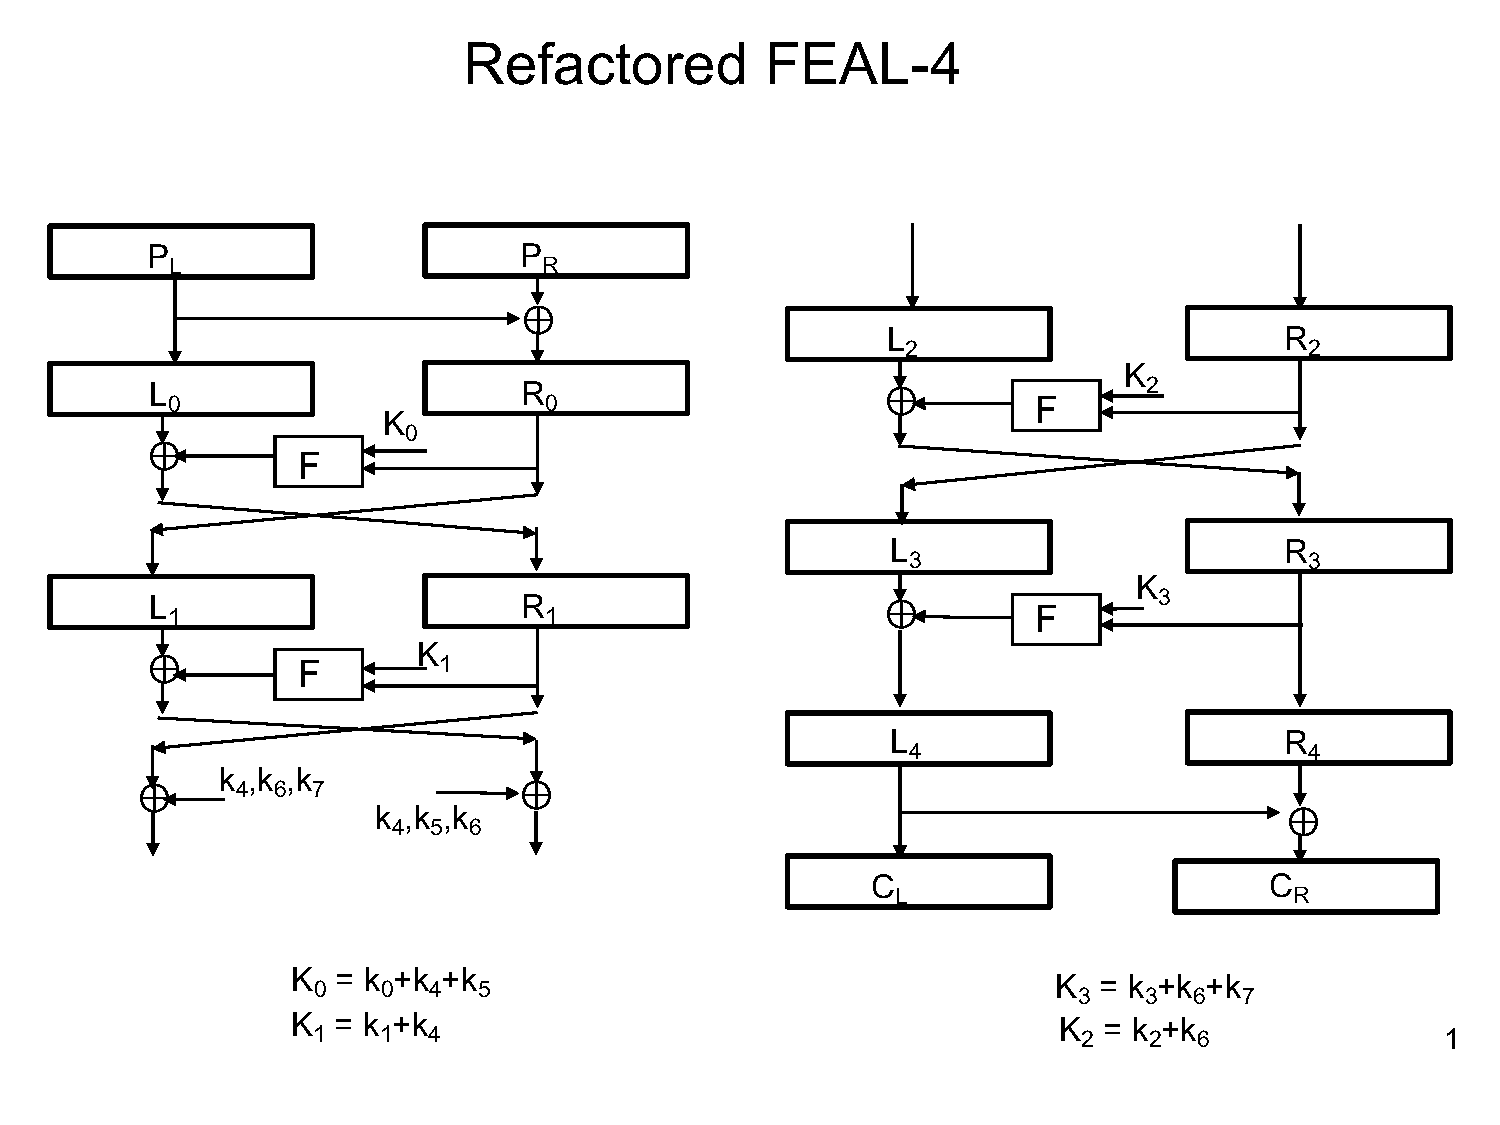
\includegraphics[width=0.8\textwidth,natwidth=642,natheight=610, height=80mm, width=88mm]{feal1.pdf}
\end{figure}
\begin{figure} 
\center
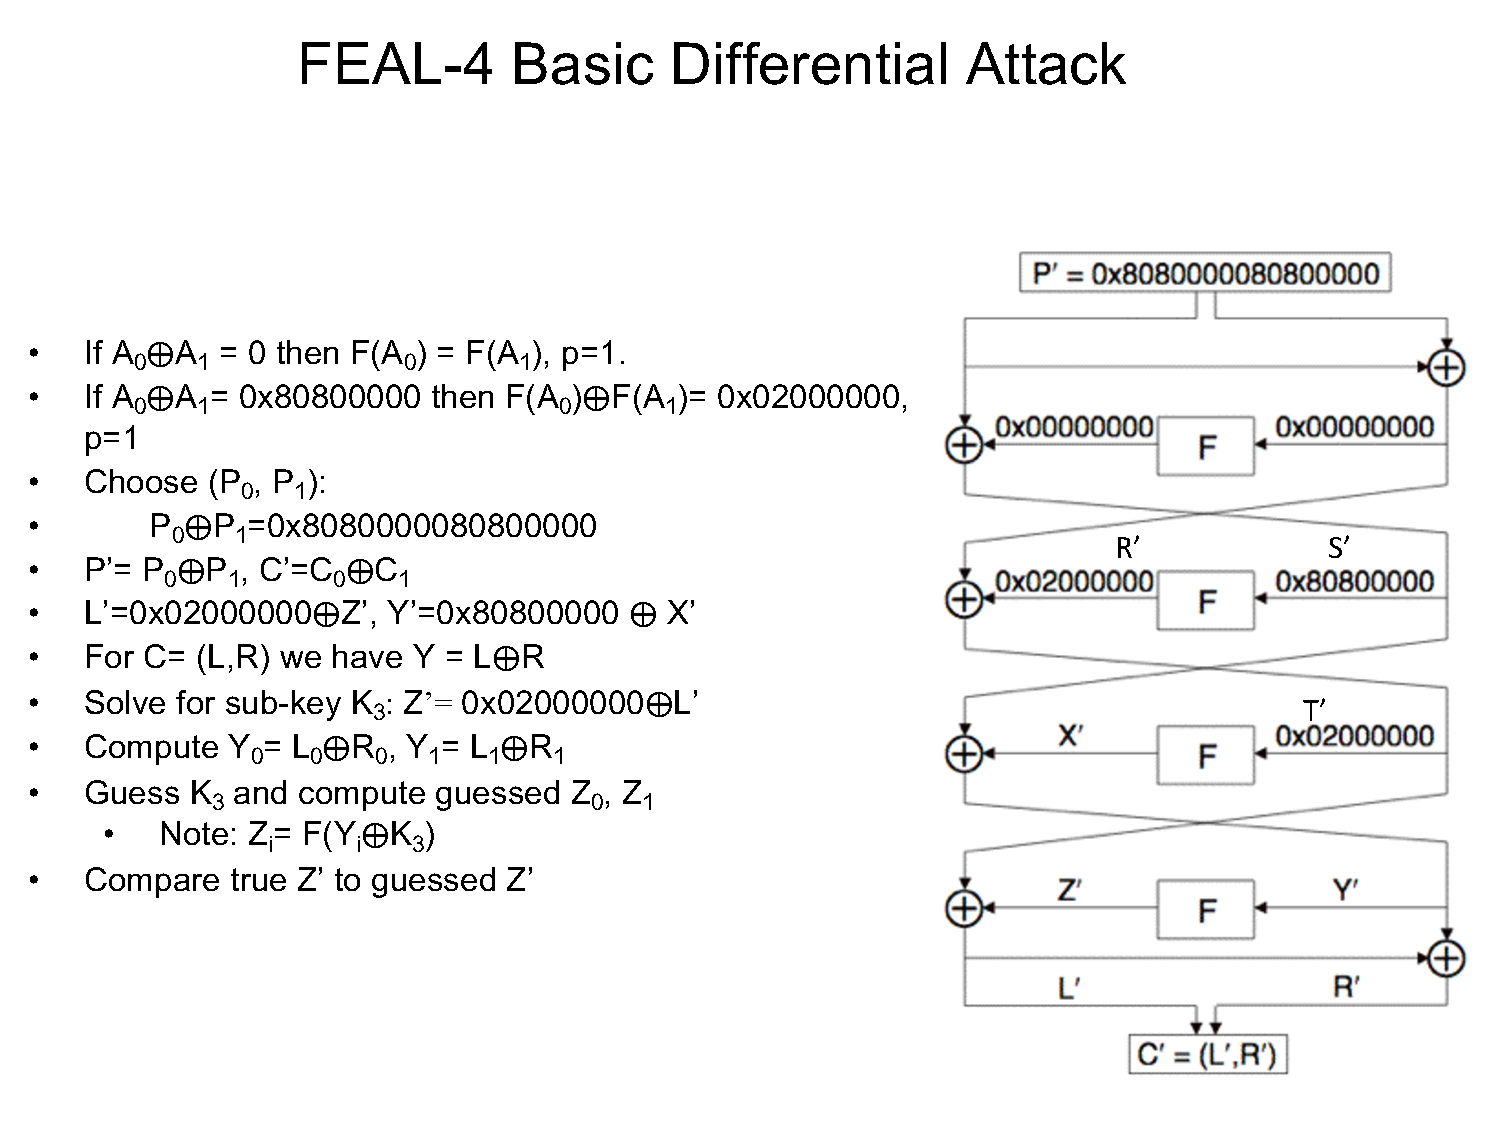
\includegraphics[width=0.8\textwidth,natwidth=642,natheight=610, height=80mm, width=88mm]{feal2.pdf}
\end{figure}
\\
{\bf RC4 Weakness:}  Let $S_i$ be the state at time $i$, $N= 2^n$ ($n=8$,
usually).
Let $\langle z_i \rangle$ be the output sequence.  $P(z_2=0)= {\frac 2 N}$.
[\emph{Proof:} Suppose $S_0[2]=0$, $S_0[1] \ne 2$, $S_0[1]= X$, $S_0[X]= Y$.]
Round 1:
$i=1$, $X=S_0[1]+0$.  Exchange $S_0[1]$ and $S_0[Y]$.  Round 2: $i=2$,
$j= X+S_1[2]=X$,  Output $S_1[S_1[2]+S_1[X]]= S_1[X]= 0$.  So
$P(z_2 = 0) \approx {\frac 1 N} + {\frac 1 N} (1- {\frac 1 N}) \approx
{\frac 2 N}$.  So by Bayes, if $z_2= 0$, we can extract byte of state with
probability ${\frac 1 2}$.
\\
\\
{\bf WEP Attack:}
WEP is data level encryption using a long term secret $K$ and per message initial vector,
$IV$ which is $3$ bytes which we call $K_0, K_1, K_3$.  The IV and the key bytes $K_3, ...$
form a single RC4 key $K_0, K_1, K_2, K_3, \ldots$.  Attack involves selecting $IV= 3|255|V$.
The RC4 initialization at $i=0$ step is
$j= j+S_0+255 = 3 \jmod {256}$ then swap $S[0], S[3]$; this leaves $S$:
\begin{center}
\begin{tabular} {|l|r|r|r|r|r|r|r|r|r|}
\hline
i & 0 & 1 & 2 & 3 & 4 & 5 & 6 & 7 & ... \\
\hline
S[i] & 3 & 1 & 2 & 0 & 4 & 5 & 6 & 7 & ... \\
\hline
\end{tabular}
\end{center}
The $i=1$ step is
$j= j+S_1+K_1 = 3+1+255 \jmod {256}= 3$; this leaves $S$:
\begin{center}
\begin{tabular} {|l|r|r|r|r|r|r|r|r|r|}
\hline
i & 0 & 1 & 2 & 3 & 4 & 5 & 6 & 7 & ... \\
\hline
S[i] & 3 & 0 & 2 & 1 & 4 & 5 & 6 & 7 & ... \\
\hline
\end{tabular}
\end{center}
The $i=2$ step is
$j= j+S_2+K_2 = 5+V \jmod {256}= 3$; this leaves $S$:
\begin{center}
\begin{tabular} {|l|r|r|r|r|r|r|r|r|r|}
\hline
i & 0 & 1 & 2 & 3 & 4 & ... & 5+V & ... & ... \\
\hline
S[i] & 3 & 0 & 5+V & 1 & 4 & ... & 2 & ... & ... \\
\hline
\end{tabular}
\end{center}
Finally, at $i=3$ step is
$j= j+S_3+K_3 = 5+V+S_3+k+3 \jmod {256}= 6+V+K_3$; this leaves $S$:
\begin{center}
\begin{tabular} {|l|r|r|r|r|r|r|r|r|r|r|}
\hline
i & 0 & 1 & 2 & 3 & 4 & ... & 5+V & ... & 6+V+K[3] & ... \\
\hline
S[i] & 3 & 0 & 5+V & 6+V+K[3] & 4 & ... & 2 & ... & 1 & ... \\
\hline
\end{tabular}
\end{center}
$Stream[0]= S[3]=6+V+K_3$ if initialization stops here.  Attack works if
$S[0], S[1], S[2]$
don't change.  The probability of this is ${\frac {253} {256}}^{255} \approx .0513$.
\\
\\
$\Delta^{\otimes}X =  X \otimes X^{-1}$.  $r-$round characteristic:  sequence of differences
$\langle \alpha_0, \alpha_1 , \ldots , \alpha_r \rangle$.
{\bf Definition (Lai):} An iterated cipher is called a Markov cipher if 
$Pr( \Delta C_1= \beta | \Delta C_0= \alpha, C_0= \gamma)$ is independent of 
$\gamma, \forall \alpha , \beta \ne e$.  \emph{Homogeneous Markov Chain:}
$Pr(v_{i+1} | v_i= \alpha)$ is independent of $i, \forall \alpha, \beta$.
\\
\\
{\bf Theorem:}
If an $r-$round iterated cipher is a Markov and the $r$ round keys are independent and
uniformly distributed then $\Delta P= \Delta C_0, \Delta C_1 , \ldots, \Delta C_r$
is a homogeneous Markov chain and
$Pr(\Delta C_s = \alpha_s | \ldots | \Delta C_1= \alpha_1 | \Delta P= \alpha_0)
= \prod Pr(\Delta C_i | \Delta C_{i-1})$.
\\
\\
{\bf Definitions:}
Let $P= (p_{ij})$ be the transition probabilities of a homogeneous Markov chain and
${p_{ij}}^s$ is the probability that state $j$ can be reached from state $i$ in
$s$ steps.  A Markov chain is \emph{ergodic} if it is aperiodic and irreducible.
If a random cipher is selected from $\Sigma_{2^n}$, $Pr( P$ is ergodic $) \rightarrow 1$.
\\
\\
{\bf Theorem (OConner):} Most Feistel ciphers are resistant to differential attack.  Let
$p_g$ be the probability of the best linear approximation of $g$.
$|p_g - {\frac 1 2}| = max_k (max_{\alpha \ne 0 \ne \beta} | Pr_x(g(x,h) \cdot \beta 
= x \cdot \alpha)- {\frac 1 2}|)$ and the best $s$ round linear approximation
satisfies $|p_L -{\frac 1 2}|^2 \le |p_g - {\frac 1 2}|^2$.  For DES, $s \ge 4$,
$|p_L - {\frac 1 2}|^2 \le 8|p_f -{\frac 1 2}|^4$.
\\
\\
{\bf Definitions:}
An $r-$round iterated $2m$ bit block cipher with $r$-round keys each has
$n$ bits.  A \emph{strong key schedule} is one in which
(1) For any $s$ bits of the $r$ round keys derived from $k$ where $s<rn$, it is ``hard''
to find any of the remaining $rn-s$ bits from the $s$ bits, (2) given a relation between
two different master keys, is it ``hard'' to predict the relationship between any of the 
round keys.  $\langle RK_l \rangle= n MSB(E_{k_i}(IV \oplus l))$.
\\
\\
\section{New Ciphers}
\subsection{AES-Rijndael}
Arithmetic in $GF(2^8 )$ with minimum polynomial $m(x)= x^8 + x^4 +x^3 +x
+1$.  If $m(\theta)=0$, matrix for multiplication by $\theta$ over $GF(2)$ is denoted
by $T$ and squaring by $S$, then
$$
T=
\left(
\begin{array}{cccccccc}
0 & 1 & 0 & 0 & 0 & 0 & 0 & 0 \\
0 & 0 & 1 & 0 & 0 & 0 & 0 & 0 \\
0 & 0 & 0 & 1 & 0 & 0 & 0 & 0 \\
1 & 0 & 0 & 0 & 1 & 0 & 0 & 0 \\
1 & 0 & 0 & 0 & 0 & 1 & 0 & 0 \\
0 & 0 & 0 & 0 & 0 & 0 & 1 & 0 \\
1 & 0 & 0 & 0 & 0 & 0 & 0 & 1 \\
1 & 0 & 0 & 0 & 0 & 0 & 0 & 0  
\end{array}
\right), 
S=
\left(
\begin{array}{cccccccc}
1 & 1 & 0 & 0 & 0 & 0 & 0 & 0 \\
0 & 0 & 1 & 0 & 1 & 0 & 0 & 0 \\
0 & 1 & 1 & 0 & 0 & 0 & 0 & 0 \\
1 & 0 & 0 & 1 & 0 & 1 & 0 & 0 \\
1 & 1 & 1 & 1 & 0 & 0 & 0 & 0 \\
0 & 0 & 1 & 0 & 0 & 0 & 1 & 0 \\
1 & 1 & 0 & 1 & 0 & 0 & 0 & 0 \\
0 & 1 & 0 & 1 & 0 & 0 & 0 & 1  
\end{array}
\right)
$$  
$Tr(a)= a + a^p + a^{p^2} + \ldots + a^{p^{d-1}}$ and
$N(a)= a  a^p  a^{p^2}  \ldots  a^{p^{d-1}}$.
Linearized polynomial: $L(x)= a_0 x + a_1 x^p + a_2 x^{p^2} + \ldots + a_{d-1} x^{p^{d-1}}$;
linear functions can be expressed as linearized polynomials.
\\
\\
{\bf Rijndael} input: $p$ consisting of $Nb$ words, $k$ with $Nk$ words.
State: 4 rows, $Nb$ columns.
Key: 4 rows, $Nk$ columns.
Both key rows are filled in the following order:
Fill leftmost column $s_{i,0}, i= 0, 1, 2, 3$,
then next column, etc.
\begin{multicols} {2} {
\begin{verbatim}
    Nb/Nk  4   6   8
       4  10  12  14 
       6  12  12  14 
       8  14  14  14 

Rijndael(p, k, Nb, Nk)  {
    ComputeRoundKeys(K, W[i])
    state= p 
    AddRoundKey(state)
    for (i=0, i<Nr, i++) {
         for each byte, b in state, ByteSub(b)
         ShiftRow(state)
         if(i<Nr-1) 
             MixCol(state)
         AddRoundKey(state)
         }
}

ByteSub(b) {
    t= 0 
    if b!=0 {
        t= 1/b;
    // M= circ(1,0,0,0,1,1,1,1) 
    // [Shift right going down].
    // a= (1,1,0,0,0,1,1,0)^T.
    return(Mt + a);
    }

ShiftRow(state) {
    shift right row 1 by 0. 
    shift right row 2 by 1. 
    shift right row 3 by 2 if Nb<8, 
                      3 otherwise. 
    shift right row 4 by 3 if Nb<8, 
                      4 otherwise. 
    }

MixCol(state) {
    multiply each col of state by 
             c(x) (mod  x**4+1);
    // c(x)= 0x03x**3+0x01x**2+0x01x+0x02
    // d(x)= 0x0bx**3+0x0dx**2+0x09x+0x0e
    }

AddRoundKey(state) {
    state= state + W[i];
    }

ComputeRoundKeys(K[4*Nk], W[Nb*(Nr+1)]) {
    for(i=0; i<Nk; i++) 
           W[i]= (K[4i], K[4i+1], 
                  K[4i+2], K[4i+3])
    for(i=Nk; i<Nb*(Nr+1)); i++) {
        t= W[i-1];
        if((i mod Nk)==0)
           t= SubByte(RotByte(t))^RCon(i/Nk);
        if((i mod Nk)==4 and Nk>6)
           t=SubByte(t);
        W[i]= W[i-Nk] ^ t;
        }
    }

SubByte(w) {
    w= ByteSub(w);
    }

RotByte(w= (a,b,c,d)) {
    w= (b,c,d,a);
    }

RCon[i]= (RC[i], 0x00, 0x00, 0x00);
RC[1]= 0x01;
RC[i+1]=  RC[i]*x (x in poly over GF(2));
\end{verbatim}
}
\end{multicols}
Note $[ShiftRow, MixCol]=1$.  Rounds Key: $ K_{r,0}, K_{r,1}, \ldots , K_{r,15}$.
First Round is input key.  For $s= r+1$, 
$T_0 = S[K_{r,13}] + \theta^r$,
$T_1 = S[K_{r,14}]$,
$T_2 = S[K_{r,15}]$,
$T_3 = S[K_{r,12}]$ and 
$K_{s,i}= K_{r,i}+T_i, 0 \le i \le 3$, 
$K_{s,i}= K_{r,i}+K_{s, i-4}, 4 \le i \le 15$.  Note that key expansion is
equivalent to: 
$W[i]= W[i-1] \oplus W[i-4]$, if $i \ne 0 \jmod{4}$
$W[i]= T(W[i-1]) \oplus W[i-4]$, if $i = 0 \jmod{4}$ where
$T(a,b,c,d)= 
(SB(b) \oplus r(i), SB(c), SB(d), SB(a)), r(i)= 0x02^{\frac {i-4} 4}$
in $GF(2^8)$.
Inverse provides linear/differential immunity,
linear diffusion provides algebraic complexity.
\\
\\
$$
L=
\left(
\begin{array}{cccccccc}
1 & 0 & 0 & 0 & 1 & 1 & 1 & 1 \\
1 & 1 & 0 & 0 & 0 & 1 & 1 & 1 \\
1 & 1 & 1 & 0 & 0 & 0 & 1 & 1 \\
1 & 1 & 1 & 1 & 0 & 0 & 0 & 1 \\
1 & 1 & 1 & 1 & 1 & 0 & 0 & 0 \\
0 & 1 & 1 & 1 & 1 & 1 & 0 & 0 \\
0 & 0 & 1 & 1 & 1 & 1 & 1 & 0 \\
0 & 0 & 0 & 1 & 1 & 1 & 1 & 1  
\end{array}
\right), 
\left(
\begin{array}{c}
y_7 \\
y_6 \\
y_5 \\
y_4 \\
y_3 \\
y_2 \\
y_1 \\
y_0
\end{array}
\right)
= L
\left(
\begin{array}{c}
x_7 \\
x_6 \\
x_5 \\
x_4 \\
x_3 \\
x_2 \\
x_1 \\
x_0
\end{array}
\right)
$$
$S[w]= L[w^{(-1)}] + 0x63$.   Combined RowShift, ColumnMix and Diffusion and AddRound is
$x \mapsto Mx + 0x63 + k_i$ where $M$ is a $16 \times 16$ matrix and
$min_M (x)= (x+1)^{15}) | (x^{16} +1)$ which can be transformed into
$P^{-1} M P= V_1 \oplus \ldots \oplus V_{15}$ with $dim(V_i)= (16, 14^3, 10^3, 8^2,6,4,4^4,2)$.
\\
\\
{\bf AES Design Overview:}
\emph{Linear cryptanalysis resistance for AES design} is provided if no linear trail has a
correlation coefficient $>2^{\frac n 2}$.  \emph{Differential cryptanalysis resistance} is
provided if there is no differential trail with prop ratio $>2^{1-n}$.  
The \emph{prop ratio} of differential trail is 
approximately the product of the prop ratios of its active S-boxes.
The \emph{correlation} of a linear trail is approximately the 
product of the I/O correlations of its active S-boxes.  
The \emph{wide trail} strategy is: (1) choose an S-box with maximum
prop ratio and correlation $\approx 2^{-6}, 2^{-3}$, respectively; 
(b) construct diffusion layer
in such a way that there are no multiple round trails with few active S-boxes.
\\
\\
{\bf Theorem:}
The weight of a two round trail with $Q$ active columns at the input 
and output is $\ge 5Q$; The minimum number of active 
S-boxes in a four round differential or linear trail is $25.$
\subsection{Tea, TwoFish}
\begin{verbatim}
Tea(unsigned K[4], ref unsigned L, ref unsigned R) {
    unsigned d= 0x9e3779b9;
    unsigned s= 0;
    for(int i=0; i<32;i++) {
        s+= d;
        L+= ((R<<4)+K[0])^(R+s)^((R>>5)+K[1]);
        R+= ((L<<4)+K[2])^(L+s)^((L>>5)+K[3]);
        }
    }
\end{verbatim}
(1) 4 different $8 \times 8$ bijective, key dependent S boxes.
(2) MDS code.
(3) PHT: $a'= a+b \jmod{2^{32}}$,
$b'= a+2b \jmod{2^{32}}$.
Basic algorithm: whiten, 16 rounds, whiten. \\
$$
MDS= 
\left(
\begin{array}{cccc}
0x01 & 0xef & 0x5b & 0x5b\\
0x5b & 0xef & 0x5b & 0x01\\
0xef & 0x5b & 0x01 & 0xef\\
0xef & 0x01 & 0xef & 0x5b\\
\end{array}
\right)
$$
$Round(w_1 , w_2 , w_3 , w_4 , k_1 , k_2 )= (w_1 ', w_2 ', w_1 , w_2 )$:
$w_1 '= w_3 + F_1 (w_1 , w_2 , r) >>> 1$;
$w_2 '= (w_4 <<< 1)+ F_1 (w_1 , w_2 , r)$;
$F_r (w, v) = PHT(g(w), g(v<<<8)) + k_r \jmod{2^{32}}$;
$g(x, y, z,w) = MDS 
\left(
\begin{array}{c}
S_1 (x) \\
S_2 (y) \\
S_3 (z) \\
S_4 (w) \\
\end{array}
\right)$.  All calculations over $GF(2^8 )$.
\subsection{Miscellaneous}
{\bf Cramer-Shoup:} $G= {\mathbb Z}_p$, $G= \langle g \rangle= \langle g' \rangle$, $H$, 
a collision resistant hash whose
image is ${{\mathbb Z}_p}^*$.  $PK= (G, g, g', h, k, k')$, $s, t, t', u, u'$ randomly
selected.  $h=sg$, $k=tg+t'g'$, $k'=ug+u'g'$.  Encrypt (m): Choose $r$,
random,
set $n= H(rg | rg' | m+rnk')$.
$E(m)= (x, y, z, w)= (rg, rg', m+rh, rk+rnk')$. Decryption: $D(x, y, z, w)$,
check that $(nu+t)x + (nu'+t'))y=w$.  If so, compute $z-sx$.
\\
\\
{\bf Bit Commitment and coin flips:} $b, b' \in \{0,1\}$. Alice sends Bob
$c=commit(b)$, Bob sends Alice $b'$, Alice sends Bob $reveal(c)$.  Result is
$b \oplus b'$.
\\
\\
{\bf Zero Knowledge} using 3 color:  For each round, Prover randomly permutes colors
and $commits$ color at each vertex.  For each round, Verifier asks to
$reveal$ color at the vertices of an edge.
blob: commit with equality.
\\
\\
{\bf Shalevi-Micali Commit:} $h$ is a one way function like $SHA1$.
$commit(m)= h(r||m)$, $r$, random.  $p$ a 161 bit prime.  Pick
$a, b$: $ax+b=z \jmod{p}, y=h(x), c=(y,a,b)$.  $reveal(c)= x,m$.
\\
\\
{\bf Time memory tradeoff:}
Fix a plaintext block, $P$ and pick $SP_{i}, i= 1,2, \ldots, m$.
For each $i$, set $K_0^i = SP_i$ and $K_{j+1}^i= F(E(K_j^i, P)), j= 0, 1, \ldots , t-1$
where $F$ is a randomizing function to avoid short cycles and put $EP_i=K_t^i$.  
For each $i$, store $(SP_i, EP_i)$. Phase 2: Get $C=E(P, K)$ from oracle
where $K$ is unknown.  Compute
$X_0= C$, $X_{i+1}= E(P, X_i)$ until $X_i= EP_j$ for some $i, j$.
Then compute $Y_0= EP_j$ and $Y_{j+1}= E(P, Y_j)$ until $Y_k = C$ then
$K= Y_{k-1}$.  If $m$ is the number of starting points for each $F$, $t$ is the number of
encryptions per chain and $r$ is the number of tables.  Attack requires $mr$ memory
and $tr$ time with the probability of success $1- e^{-{\frac {trm} k}}$.
\\
\\
{\bf Nostradamus (``herding'') attack:}  Let $h$ be a
Merkle-Damgard hash with compression function $f$ and initial value $IV$.
Goal is to hash a prefix value (P) quickly by appending random suffixes (S).
Procedure Phase 1:  Pick $k$ and generate $2^k$ random values $d_{0i}$ from each pair of
the values $f(IV||d_{i, i+1})$ find two messages 
$M_{0,j}, M_{1,j}$ 
which collide under $f$ and call this value $d_{1,j}$
this takes effort $2^{n/2}$ for each pair.  Keep doing this (colliding
$d_{i,j}, d_{i+1,j}$ under $M_{i,j}, M_{i+1,j}$ to produce $d_{i, j+1}$
until you reach $d_{2^k , 0}$.  This is the diamond.  Publish $y= w(d_{2^k , 0})$
where $w$ is the final transformation in the hash as the hash (i.e. - claim $y=h(P||S)$.
The cost of phase 1 is $(2^k-1) 2^{n/2}$.  In phase 2, guess $S'$ and compute
$T= f(IV||P||S')$; keep guessing until $T$ is one of the $d_{ij}$.  Once you get a 
collision, follow a path through the $M_{ij}$ to $d_{2^k, 0}$, append these $M_{ij}$ to
$P||S'$ and apply $w$ to get right hash.
\section{Cryptographic Hashes}
{\bf Weak collision resistance:} Given $x$, it is computationally infeasible to
find $x' \ne x$ with $h(x)=h(x')$.
{\bf Strong collision resistance:} It is computationally infeasible to
find $x' \ne x$ with $h(x)=h(x')$ for any $x$, $x'$.  
{\bf One-way:} Given a
digest $z$, it is computationally infeasible to find $x$ with $h(x)=z$.
Strongly collision resistant implies one-way. \\
\\
{\bf Merkle Damgard construction:}  $z_0= IV, z_{i+1}= f(z_i, m_i), h(m)= g(z_r)$,
where $f$ is a compression function, $r$ is the number of rounds and
$m= m_1 || m_2 || \ldots || m_r$.  If $f$ is
collision resistant then so is $h$.
{\bf Hash from Block Cipher:} $m= m_1 || m_2 || \ldots || m_r$,  $H_0 = IV$, $H_i = E_{m_i}(H_{i-1}) \oplus H_{i-1}$,
$H(m)= f(H_i)$.  is the Meyer-Davis construction.\\
$g_i = e_{g_{i-1}} (x_i ) + x_i $,
$g_i = e_{g_{i-1}} (x_i ) + x_i + g_{i-1}$,
$g_i = e_{g_{i-1}} (g_{i-1} + x_i ) + x_i $,
$g_i = e_{g_{i-1}} (g_{i-1} + x_i ) + g_{i-1} + x_i $.
\\
\\
{\bf Chaum Hash:} $\alpha$,
$\beta$ two primitive elements of ${\mathbb Z}_p$,
$h(x,y)= \alpha^{x} \beta^{y} \jmod{p}$.  If there's a collision,
$log_{\alpha} (\beta )$ can be computed efficiently. $h(0^{t+1} || y_1)$,
$g_{i+1} = h(g_i || 1 || y_{i+1})$. Do reduction proof.
\\
\\
{\bf Iterative construction is vulnerable to multi-collision (Joux):}  Suppose
$M_1,M_1'; M_2,M_2'; \ldots ; M_t,M_t'$ all collide.  From these we get  $2^t$ collisions.  
If $r$ people each have one of $N$ possible birthdays, there is a greater than $.5$ chance
of $k$ collisions if
$r > N^{\frac {k-1} k}$.  Prove this fact.
\\
\\
{\bf Random Oracle Model:} 
Let $f$ be a OWF with trapdoor, $(y_1, y_2)= (f(r) , h(r) + m)$ is used as encryption.
An oracle with $l$ requests $L$, $Pr(guess \; right)= P( r \in L) + {\frac 1 2} P( \neg r \in L)$.  
Set $p= {\frac 1 2}+e$,
$e \le Pr(r \in L)$.  
Canetti, Goldreich, Halevi constructed a cryptosystem that is secure in Random Oracle Model but 
insecure for any concrete hash.
\\
\\
{\bf MD-4:}  In description below, K[0]= 0, K[1]= 0x5a827999, K[2]= 0x6ed9eba1.
$F(A,B,C) = (A \wedge B) \vee (\neg A \wedge C)$,
$G(A,B,C) = (A \wedge B) \vee (A \wedge C) \vee (B \wedge C)$,
$H(A,B,C) = (A \oplus B) \oplus C$.  $W_i= X_{\sigma(i)}, i= 0, 1, \ldots, 47$.
$Q_{-4}= A$,
$Q_{-3}= D$,
$Q_{-2}= C$,
$Q_{-1}= B$.
$Q_i(A,B,C)= (Q_{i-4} + F(Q_{i-1}, Q_{i-2}, Q_{i-3}) + W_i + K_0)<<<s_i, 0 \le i \le 15$,
$Q_i(A,B,C)= (Q_{i-4} + G(Q_{i-1}, Q_{i-2}, Q_{i-3}) + W_i + K_1)<<<s_i, 16 \le i \le 31$,
$Q_i(A,B,C)= (Q_{i-4} + H(Q_{i-1}, Q_{i-2}, Q_{i-3}) + W_i + K_2)<<<s_i, 32 \le i \le 47$.
\begin{verbatim}
MD-4(Y[0] , ..., Y[N-1])
    K[0]= 0; K[1]= 0x5a827999; K[2]= 0x6ed9eba1; 
    (A, B, C, D)= (0x67452301, 0xefcdab89, 0x98badcfe, 0x10325476);
    for(i=0; i<(N/16); i++) {
        X[j]= Y[16i+j], j= 0, 1, ..., 15;
        W[j]= X[SIGMA(j)], j= 0, 1, ..., 47;
        Q[-4]= A;
        Q[-3]= D;
        Q[-2]= C;
        Q[-1]= B;
        // Calculate Q[i] recursively according to formula above
        (A, B, C, D)+= (Q[44], Q[45], Q[46], Q[47]);
        (A, B, C, D)= (A, D, C, B);
        }
    return (A, B, C, D);
\end{verbatim}
{\bf Dobbertin attack on MD4, steps 20-35}  
Let $M$ and $M'$ be $512$ bit messages consisting
of $16$, $32$-bit works $X_0 , X_1 , \ldots, X_{15}$ with $X_i=X_i'$ for all $i$ except
$i=12$ and let $X_{12}' = X_{12}+1 \jmod {2^{32}}$.  We want to find a collision.
$\Delta_i= (Q_j'- Q_j, Q_{j-1}'-Q_{j-1}, Q_{j-2}'-Q_{j-2}, Q_{j-3}' - Q_{j-3})$ after
step $i$.  Dobbertin attack consists of three steps: (1) Show that if
$\Delta_{19}= (0, 2^{25}, -2^5,0)$ then $\Delta_{35}= (0, 0, 0, 0)$ with probability
$p> 2^{-30}$ (actually,
$p> 2^{-22}$); (2) get conditions on $M$ (i.e. on the $X_i$) based on
round $12$, that guarantee $\Delta_{19}= (0, 2^{25}, -2^5,0)$; (3)
find $X_0, X_1, \ldots , X_{11}$ that produce candidates that present the desired
conditions at step $12$, after about $2^{22}$ of these, you'll get a collision.
The work factor is about $2^{20}$. \\
{\bf 1.}  Steps 19-35.  Suppose 
$\Delta_{19}= (0, 2^{25}, -2^5,0)$ and 
$G(Q_{19}, Q_{18}, Q_{17})= G(Q_{19}', Q_{18}', Q_{17}')$, then the following table
holds:
\begin{center}
\begin{tabular} {|r|rrrr|rrcc|}
\hline
$j$&$\Delta(Q_{j})$&$\Delta(Q_{j-1})$&$\Delta(Q_{j-2})$&$\Delta(Q_{j-3})$&$i$&$s_j$&$p$&In\\
\hline
$19$& $2^{25}$&$-2^5$&$0$&$0$&$*$&$*$&$*$&$*$\\
$20$& $0$&$2^{25}$&$-2^5$&$0$&$1$&$3$&$1$&$X_{1}$\\
$21$& $0$&$0$&$2^{25}$&$-2^5$& $1$&$5$&${\frac 1 9}$&$X_{5}$\\
$22$& $-2^{14}$&$0$&$0$&$2^{25}$& $1$&$9$&${\frac 1 3}$&$X_{9}$\\
$23$& $2^6$&$-2^{14}$&$0$&$0$& $1$&$13$&${\frac 1 3}$&$X_{13}$\\
$24$& $0$&$2^6$&$-2^{14}$&$0$& $1$&$3$&${\frac 1 9}$&$X_{2}$\\
$25$& $0$&$0$&$2^6$&$-2^{14}$& $1$&$5$&${\frac 1 9}$&$X_{6}$\\
$26$& $-2^{23}$&$0$&$0$&$2^6$& $1$&$9$&${\frac 1 3}$&$X_{10}$\\
$27$& $2^{19}$&$-2^{23}$&$0$&$0$& $1$&$13$&${\frac 1 3}$&$X_{14}$\\
$28$& $0$&$2^{19}$&$-2^{23}$&$0$& $1$&$3$&${\frac 1 9}$&$X_{3}$\\
$29$& $0$&$0$&$2^{19}$&$-2^{23}$& $1$&$5$&${\frac 1 9}$&$X_{7}$\\
$30$& $-1$&$0$&$0$&$2^{19}$& $1$&$9$&${\frac 1 3}$&$X_{11}$\\
$31$& $1$&$-1$&$0$&$0$& $1$&$13$&${\frac 1 3}$&$X_{15}$\\
$32$& $0$&$1$&$-1$&$0$& $2$&$3$&${\frac 1 3}$&$X_{0}$\\
$33$& $0$&$0$&$1$&$-1$& $2$&$9$&${\frac 1 3}$&$X_{8}$\\
$34$& $0$&$0$&$0$&$1$& $2$&$11$&${\frac 1 3}$&$X_{4}$\\
$35$& $0$&$0$&$0$&$0$& $2$&$15$&$1$&$X_{12}, X_{12}+1$\\
\hline
\end{tabular}
\end{center}
{\bf Steps 12 to 19}.
To get $\Delta_{19}= (0, 2^{25}, -2^5,0)$,
$Q_{16}=Q_{16}'$,
$Q_{19}=Q_{19}' + 2^{25}$,
$Q_{18} + 2^5 =Q_{18}'$,
$Q_{17}=Q_{17}'$  and
$Q_{i}=Q_{i}', 8 \le i \le 11$.
\begin{center}
\begin{tabular} {|r|ccc|}
\hline
$j$&$i$&M In & M' In\\
\hline
12 &0&$X_{12}$&$X_{12}+1$\\
13 &0&$X_{13}$&$X_{13}$\\
14 &0&$X_{14}$&$X_{14}$\\
15 &0&$X_{15}$&$X_{15}$\\
16 &1&$X_{0}$&$X_{0}$\\
17 &1&$X_{4}$&$X_{4}$\\
18 &1&$X_{1}$&$X_{8}$\\
19 &1&$X_{12}$&$X_{12}+1$\\
\hline
\end{tabular}
\end{center}
These yield the following conditions:
$(Q_{12}' <<< 29) - (Q_{12} <<< 29) =1$,
$F(Q_{12}', Q_{11}, Q_{10}) - F(Q_{12}, Q_{11}, Q_{10})= (Q_{13}'<<<25) - (Q_{13}<<<25)$,
$F(Q_{13}', Q_{12}, Q_{11}) - F(Q_{13}, Q_{12}, Q_{11})= (Q_{14}'<<<21) - (Q_{14}<<<21)$,
$F(Q_{14}', Q_{13}, Q_{12}) - F(Q_{14}, Q_{13}, Q_{12})= (Q_{15}'<<<13) - (Q_{15}<<<13)$,
$G(Q_{15}', Q_{14}', Q_{13}) - G(Q_{15}, Q_{14}, Q_{13})= Q_{12} - (Q_{12}'$,
$G(Q_{16}', Q_{15}', Q_{14}) - G(Q_{16}, Q_{15}, Q_{13})= Q_{13} - (Q_{13}'$,
$G(Q_{17}', Q_{16}', Q_{15}) - G(Q_{17}, Q_{16}, Q_{14})= 
Q_{12} - Q_{12}' + (Q_{18} <<< 23) - (Q_{18} <<< 23)'$,
$G(Q_{18}', Q_{17}', Q_{16}) - G(Q_{18}, Q_{17}, Q_{15})= 
Q_{15} - Q_{15}' + (Q_{19} <<< 19) - (Q_{19} <<< 19)')$.  
Choose $Q_{14}, Q_{15}, \ldots , Q_{19}$ arbitrarily and solve for
$
Q_{10}, Q_{13},
Q_{13}', Q_{14}',
Q_{15}'$, use the $Q$'s to solve for $X_j , j= 0, 4, 8, 12, 13, 14, 15$.
For the solutions,
$$(Q_{10}, Q_{11}, Q_{12}, Q_{13}, Q_{14}, Q_{15}, Q_{16}, 
Q_{17}, Q_{18}, Q_{19}, Q_{12}', Q_{13}', Q_{14}', Q_{15}'),$$ $\Delta_{19}$ will hold
if
$X_{13}= \; anything$,
$X_{14}= (Q_{14} <<< 21) - Q_{10} -F(Q_{13}, Q_{12}, Q_{11}) $,
$X_{15}= (Q_{15} <<< 13) - Q_{11} -F(Q_{14}, Q_{13}, Q_{12}) $,
$X_{ 0}= (Q_{16} <<< 29) - Q_{12} -G(Q_{15}, Q_{14}, Q_{13}) - K_1 $,
$X_{ 4}= (Q_{17} <<< 27) - Q_{13} -G(Q_{16}, Q_{15}, Q_{14})  - K_1$,
$X_{ 8}= (Q_{18} <<< 23) - Q_{14} -G(Q_{17}, Q_{16}, Q_{15})  - K_1$,
$X_{12}= (Q_{19} <<< 19) - Q_{15} -G(Q_{18}, Q_{17}, Q_{16})  - K_1$,
$Q_{ 9}= (Q_{13} <<< 25) -F(Q_{12}, Q_{11}, Q_{10}) - X_{13}$,
$Q_{ 8}= (Q_{12} <<< 19) -F(Q_{11}, Q_{10}, Q_{09}) - X_{12}$.  Can choose
$Q_{12}= -1$, $Q_{12}'=0$, $Q_{11}=0$ to simplify.
This means we can pick
$Q_{14}, Q_{15}, Q_{16}, Q_{17}, Q_{18}, Q_{19}$ 
arbitrarily and determine
$Q_{10}, Q_{13}, Q_{13}', Q_{14}', Q_{15}'$ subject to the checks
$ G(Q_{15}, Q_{14}, Q_{13}) - G(Q_{15}', Q_{14}', Q_{13}') = 1$ and
$ F(Q_{14}', Q_{13}', 0) - F(Q_{14}, Q_{13}, -1) -
(Q_{15}' <<< 13) + (Q_{15} <<< 13) = 0$.  Finally, we must insure the solutions is
admissible by checking that
$G(Q_{19}', Q_{18}', Q_{17}) = G(Q_{19}, Q_{18}, Q_{17})$.  Under these circumstances
the solution is a candidate for the differential.  Once one candidate is found
use the ``continuity'' of $F$ and $G$ by modifying one bit of the candidate at a time,
the continuity makes it likely this will work. \\
{\bf Steps 0 to 11}.  Having found $Q_{8 }, Q_{9 }, Q_{10}, Q_{11}$ such that
$$MD4_{12, \ldots, 47}(Q_{8 }, Q_{9 }, Q_{10}, Q_{11}, X)=
MD4_{12, \ldots, 47}(Q_{8 }, Q_{9 }, Q_{10}, Q_{11}, X')$$
we need to find
$MD4_{0, \ldots, 11}(IV,X) = (Q_{11}, Q_{10}, Q_{ 9}, Q_{ 8})$.  We are free
to choose
$X_j, j= 1,2,5,6,7,9,10,11$.  We pick
$ X_{ 1}, X_{ 2}, X_{ 3}, X_{ 5} $ at random and compute
$ X_{ 6}, X_{ 7}, X_{ 9}, X_{10} , X_{11} $ such that
$MD4_{6, \ldots, 11}(Q_{2 }, Q_{3 }, Q_{ 4}, Q_{ 5}, X)=
(Q_{11}, Q_{10}, Q_{ 9}, Q_{ 8})$.  Since
$Q_{11}= (Q_{7} +F(Q_{10}, Q_{ 9}, Q_{ 8}) + X_{11}) <<<19$,
if can do this by making
$X_{11}= (Q_{11} <<< 13) - Q_{7} - F(Q_{10}, Q_{ 9}, Q_{ 8})$ and
similarly for $X_{10}, X_{9}$.  We can't do this for $X_9$ but since
$Q_{ 8}= (Q_{4} +F(Q_{ 7}, Q_{ 6}, Q_{ 5}) + X_{8}) <<< 3$, if
$Q_7= -1, Q_6= (Q_8 <<< 29) -Q_4 -X_8$ the desired equation holds for
all such $X_8$; in particular, by picking
$X_{6}= (Q_{6} <<< 21) - Q_{2} - F(Q_{5}, Q_{4}, Q_{3})$ and
$X_{7}= (Q_{7} <<< 13) - Q_{3} - F(Q_{6}, Q_{5}, Q_{4})$.  These
guarantee $\Delta_{35}= 0$.
\begin{tabbing}
\= \kill
{\bf SHA1}\= ($M$,\= $n$)  \=\\
// $M$ is message, $n$ is number of 512 bit blocks \\
    \> M= SHA1Pad(M)  \\
    \> $f_i(B,C,D)= (B \wedge C) \vee ({\overline B} \wedge D), 0 \leq i \leq 19$ \\
    \> $f_i(B,C,D)= (B \oplus C \oplus D), 20 \leq i \leq 39$\\
    \> $f_i(B,C,D)= (B \wedge C) \vee (B \wedge D) \vee (C \wedge D), 40 \leq i \leq 59$ \\
    \> $f_i(B,C,D)= (B \oplus C \oplus D), 60 \leq i \leq 79$\\
    \>\\
    \> $K_i= 0x5a827999, 0 \leq i \leq 19; K_i= 0x6ed9eba1, 20 \leq i \leq 39$\\
    \> $K_i= 0x8f1bbcdc, 40 \leq i \leq 59; K_i= 0x6a62c1d6, 60 \leq i \leq 79$\\
    \>\\
    \> $H_0= 0x67452301, H_1= 0xefcdab89 , H_2= 0x98badcfe , H_3= 0x10324576 ,
	H_4= 0xc3d2e1f0 $\\
    \>\\
    \>for (\=i=0, $i<n$, i++) \{\\
    \>     \> $M_i= W_0 || W_1 || \ldots || W_{15}$\\
    \>     \> for($j=16, j<80, j++$) \{\\
    \>     \>	\> // $ROTL^1$ below is difference between SHA-0 and SHA-1 \\
    \>     \>	\> $W_j= ROTL^1(W_{j-3} \oplus W_{j-8} \oplus W_{j-14} \oplus W_{j-16})$\\
    \>     \>	\> \}\\
    \>     \> $A= H_0, B=H_1, C=H_2, D=H_3, E=H_4$\\
    \>     \> for($j=0, j<80$; j++) \{\\
    \>     \>	\> $ROTL^5$ below is correlated to lowest wt differential \\
    \>     \>	\> $t= ROTL^5(A) + f_j(B,C,D) + E + W_j + K_j$\\
    \>     \>	\> $E= D, D=C, C=ROTL^{30}(B), B=A, A=t$\\
    \>     \>	\> \}\\
    \>	   \> $ H_0+= A, H_1+= B, H_2+= C, H_3+= D, H_4+= E $\\
    \>     \>\}
\end{tabbing}
\begin{verbatim}
SHA-1Pad(x)   // with MD strengthening
    Append 1 and enough 0's until there are 64 bits remaining 
    Append size hashed in 64 bit format 
    return(x)
\end{verbatim}
{\bf Shamir's non-linear functions with maximal period:} $x \rightarrow x^2 \wedge c$,
$x \rightarrow x + 4 h(x) +1$. \emph{Example:} $x \rightarrow (x+1)(2x+1)$.
\\
\\
{\bf SHA-3 (Keccak):}
Basic mixing function is $Keccak-f[b]$.  $b= r+c$.
$b= 25, 50, 100, 200, 400, 800, 1600$.  For SHA-3, $r=1024$, $c=576$, $b=1600$.
$w= {\frac b {25}}= 2^l$, $n_r= 12+2l$.  So for SHA-3, $n_r= 24$. State $s[b]$
is addressed by $a(x,y,z)= w(5y+x)+z$, little endian. Terminology:
row, constant $(y, z)$, column, constant $(x, z)$, lane, constant $(x, y)$.
Pad: $10^*1$.
\begin {multicols} {2} {
\begin{verbatim}
Keccak-f[r,c](A, RC)
    for(i=0;i<nr;i++)
        A= Round[b](A,RC);

rot(W,r)
    W[(i+r)(mod laneSize)]= W[i];

Round[b](A, RC)
    C[x]= A[x,0]^A[x,1]^A[x,2]^A[x,3]^A[x,4];
    D[x]= C[x-1]^rot(C[x+1], 1);
    A[x,y]= A[x,y]^D[x];
    B[y,2x+3y]= rot(A[x,y], r(x,y));
    A[x,y]= B[x,y]^(NOT(A[x,y]) AND B[x+2,y]); 
    A[0,0]= A[0,0]^RC;

    r(x,y)  x=3  x=4  x=0  x=1  x=2
    y=2      25   39    3   10   43
    y=1      55   20   36   44    6
    y=0      28   27    0    1   62
    y=4      56   14   18    2   61
    y=3      21    8   41   45   15

Keccak-f[r,c](M)
    P=M||(0x01 0x00 ... 0x00;
    P^=   0x80;
    s[i,j]= 0;

Absorb(P[i])
    s[x,y]^= P[i][x+5y];
    s= Keccak-f[r,c]

Squeeze(k)
    first k bits of s
\end{verbatim}
}
\end{multicols}

$
\left(
\begin{array}{c}
1 \\
0
\end{array}
\right)=
\left(
\begin{array}{cc}
0 & 2 \\
1 & 3 \\
\end{array}
\right)
\left(
\begin{array}{c}
x \\
y
\end{array}
\right)
$.  $rc[t]= x^t \jmod{x^8+x^6+x^5+x^4+1}$, $RC[i_r][0,0][2^j-1]= rc[j+7i_r], 0 \leq j <l$.
Distinguisher: $2^{\frac b 2}$.
Inner collision: $n^2 2^{-(c+1)}$.
State recovery: $n m 2^{-c}$.
\\
\\
{\bf Changes from MD4 to MD5:} (1) 64 steps, function for final 16 rounds is
$I(A,B,C)= B \oplus (A \vee \neg C)$, (2) $G(A,B,C)= (A \wedge C) \vee (B \wedge \neg C)$,
(3) each round uses different constant, (4) each step adds result of previous step,
(5) the order of input words to the steps is different,(6) shift values are different.
Chinese attack uses ``precise'' differential (signed difference) where $0$ indicates no difference,
$+$ indicates $1 \rightarrow 0$ difference and
$-$ indicates $0 \rightarrow 1$ difference.
This is different from both xor and modular difference; for example,
if $z'= 10100101, z= 10010101$, $\nabla(z', z)= 00+-0000$.
\\
\\
{\bf Chinese attack on MD5.}  Attack proceeds in four
phases: (1) specify input differential patters via modular difference (hard and
``done by hand'' according to Wang), (2) specify output differential pattern (only 1 known)
that is easily satisfied in earlier rounds, (3) derive sufficient conditions propagation;
(4) generate pairs of $1024$ bit numbers that satisfy 3 (deterministically when possible).
To do step 4: (a) generate $M_0$ at random; (b) use single step modification to
$M_0$ to satisfy sufficient conditions; (c) use multi-step modifications to insure
conditions hold in middle rounds; (d) check conditions for all remaining steps; (e-f)
do the same for $M_1$; compute $M_0'= M_0 + \Delta M_0$ and
$M_1'= M_1 + \Delta M_1$ according to the input differential.  
{\bf Conditions:}  $T_j= F( Q_{j-1}, Q_{j-2}, Q_{j-3}) + Q_{j-4} + K_j + W_j$, 
$R_j= T_j <<< s_j$, $Q_j= Q_{j-1} + R_j$, now apply modular difference and
derive conditions on $\Delta T_j$ and $\Delta Q_j$ for differential (below) to
hold.
\\
\\
$\Delta X = X' - X$.
$\Delta H_0 \rightarrow_{(M_0, M_0')} \Delta H_1 \rightarrow_{(M_1, M_1')} 
\Delta H_2 \ldots \rightarrow_{(M_{i-1}, M_{i-1}')} 
\Delta H_i = H$ with each composed of
$\Delta H_i \rightarrow_{P_2} \Delta R_{i+1,1} 
\rightarrow_{P_2} \Delta R_{i+1,2} \rightarrow_{P_3} \Delta R_{i+1,3} 
\rightarrow_{P_4} \Delta R_{i+1,4} = \Delta H_{i+1}$.
Let $\Delta{i,j}= x_{i,j}' - x_{i,j} = \pm 1$ and
$\Delta x_{i}[ j_1 , j_2 , \ldots , j_l ]= x_{i}[ j_1 , j_2 , \ldots , j_l] - x_{i}$.
Collision is caused by 1024 bit input: $(M_0, M_1)$ with
$\Delta M_0= (0,0,0,0,2^{31}, 0,0,0,0,0,0,2^{15},0,0,2^{31},0)$ and
$\Delta M_1= (0,0,0,0,2^{31}, 0,0,0,0,0,0,-2^{15},0,0,2^{31},0)$.  
Sufficient conditions
insure that differential holds with high probability.  At 8th iteration, 
$b_2= c_2+(b_1+F(c_2,d_2,a_2)+m_7+t_7)<<<22$,
we try to control 
$(\Delta c_2 , \Delta d_2, \Delta a_2, \Delta b_1) \rightarrow \Delta b_2$ with the
following (A) non-zero bits of $\Delta b_2$:
$d_{2,11}=1, b_{2,1}=0$,
$d_{2,26}= {\overline {a_{2,26}}}=1, b_{2,16}=0$,
$d_{2,28}= {\overline {a_{2,28}}}=0, b_{2,i}=0$,
$d_{2,11}=1, b_{2,24}=0$;
(B) zero bits of $\Delta b_2$:
$c_{2,i}=0$,
$d_{2,i}= a_{2,i}$,
$c_{2,1}=1$,
$d_{2,6}={\overline {a_{2,6}}}=0$,
$d_{2,i}= 0$,
$d_{2,12}= 1$,
$a_{2,24}= 0$, 
7th bit of $c_2, d_2, a_2$ result in no change in $b_2$.
Algorithm 1: Repeat until first block is found (a) Select random $M_0$, 
(b) Modify $M_0$,
(c) $M_0, M_0'= M_0 + \Delta M_0$ produce $\Delta M_0 \rightarrow (\Delta H_1, \Delta M_1)$
with probability $2^{-37}$, (d) Test characteristics.
2: Repeat until first block is found (a) Select random $M_1$, 
(b) Modify $M_1$,
(c) $M_1, M_1'= M_1 + \Delta M_1$ produce $\Delta M_1 \rightarrow 0$
with probability $2^{-30}$, (d) Test characteristics.
\\
\\
{\bf Comments from NIST:} Randomization (prevent offline computation for herding):
$RMX(r, M_1 | \ldots | M_L)= (r| m_1 \oplus r | \ldots | m_L \oplus r)$.
$H_r(M_1 | \ldots | M_L)= H(r| m_1 \oplus r | \ldots | m_L \oplus r)$.  Transmit $r$.
Herding attack: first committing to an output $h$, 
then mapping messages with arbitrary starting values to $h$.  Joux:  If
$H_1, H_2$ are n bit hashes;  $H_1(M) || H_2(M)$ can be broken in
$O(n2^{\frac n 2})$.  \emph{Haifa:} $h_{i+1} = CF(h_i , M_i , bitlength, salt)$.
\\
\\
{\bf Joux attack on SHA-0: }
Idea is to linearize by replacing $+$ with $\oplus$, as well as replacing $MAJ$ and $IF$
with $\oplus$.  This is ``SHI-1.''
Now select the collision in two steps.  
First, ignoring message expansion a $5$-round correction for a
local collision is: 
$\delta= W_1^{(i)} \oplus W_2^{(i)}$,
$\delta= ROL^{5}(W_1^{(i+1)} \oplus W_2^{(i+1)})$,
$\delta= W_1^{(i+2)} \oplus W_2^{(i+2)}$,
$\delta= ROL^{30}(W_1^{(i+3)} \oplus W_2^{(i+3)})$,
$\delta= ROL^{30}(W_1^{(i+4)} \oplus W_2^{(i+4)})$,
$\delta= ROL^{30}(W_1^{(i+5)} \oplus W_2^{(i+5)})$.
Since message expansion reduces the freedom of choice,
no changes can be introduced in the last $5$ rounds because there is
no way to correct them.  We focus on expansion patterns in bits $j, j+5, j+30$.
For a $5$-round correction, about ${\frac 1 {32}}$ possible ones will work beacuse they
follow the message
expansion.  Now we look at candidate collisions $(W, \Delta)$.  Taking into account
the non-linearized version, we focus on patterns in the high order bit (which has no carries) and
can calculate the probability of successful propagations of $1 \rightarrow 1$ and $1 \rightarrow 0$
transitions through $MAJ$ and $IF$.  The strategy is to choose $\Delta$ and then find $W$.
\\
\\
Attack expands by studying ``SHI-2'' which leaves $\oplus$ in SHI-1 but reintroduces
$MAJ$ and $IF$.  Effects of $MAJ$ and $IF$ are separated into four cases:
(1) No change in $b,c,d$ (the only bits affecting the $f_i$;
(2) Change in one bit of $b$;
(3) Change in one bit of $c$ or $d$;
(4) Change in one bit of each of $c$ and $d$.
``SHI-3'' takes SHI-1 and reintroduces the (non-linear) add used in calculating $a$ but leaves
$IF$ and $MAJ$'s linear replacements.  Attack gives a collision in $2^{61}$.  This was improved
by Biham and Chen by introducing ``neutral bit'' estimates and starting the perturbation later
in the rounds.
\\
\\
For SHA-0, change bit 1 (because the $+$ operation is linear in bit $1$)
which shifts to bit 31 and
is linear in $\oplus$.  Disturbance bit vector: 
$( m_{0}^{(0)}, m_{0}^{(1)}, \ldots , m_{0}^{(79)})$.  Perturbation mask:
$-5 \le i \le -1, M_{0}^{(i)}=0$,
$0 \le i \le 79, M_{0,k}^{(i)}=0$, if $k \ne 1$
$0 \le i \le 79, M_{0,1}^{(i)}= M_0^{(i)}$.  Corrective masks:
$-4 \le i \le 79, M_{1}^{(i)}= ROL_{5}(M_{1}^{(i-1)})$,
$-3 \le i \le 79, M_{2}^{(i)}= M_{1}^{(i-2)}$,
$-2 \le i \le 79, M_{3}^{(i)}= ROL_{30}(M_{1}^{(i-3)})$,
$-1 \le i \le 79, M_{3}^{(i)}= ROL_{30}(M_{1}^{(i-4)})$,
$0 \le i \le 79, M_{3}^{(i)}= ROL_{30}(M_{1}^{(i-5)})$.  
\\
\\
Early round differentials are
prescribed and later round differentials hold with non-negligible probability ($2^{-61}$,
$2^{-56}$ using \emph{neutral bits} --- A bit is neutral if flipping it doesn't change 
differential pattern).  
In Wang's multi-block attack:  patch final round errors in next block.
Early rounds are non-linear and prescribed.  Late rounds linear and probabilistic. 
\emph{Procedure:}  Fix linear characteristic, fix non-linear
characteristic, modify message (keeping differential) if conflict in mid round.
\\
\\
{\bf SHA-256 definitions:}
$Ch(x,y,z)= (x \wedge y) \oplus (\neg x \wedge z)$,  
$\psi_{256}^{i, j, k}(x)= ROTR^i (x) \oplus ROTR^j (x) \oplus ROTR^k (x)$,
$\Sigma_0^{256}(x)= \psi_{256}^{2, 13, 22} (x)$,
$\sigma_0^{256}(x)= \phi_{256}^{7, 18, 3} (x)$,
\\
{\bf SHA-512 definitions:}
$Ch(x,y,z)= (x \wedge y) \oplus (\neg x \wedge z)$,  
$\psi_{512}^{i, j, k}(x)= ROTR^i (x)  \oplus ROTR^j (x)  \oplus ROTR^k (x)$,
$\Sigma_0^{512}(x)= \psi_{512}^{28, 34, 39} (x)$,
$\Sigma_1^{512}(x)= \psi_{512}^{14, 18, 41} (x)$. \\
$\sigma_0^{512}(x)= \phi_{512}^{1,8,7} (x)$,
\begin{tabbing}
1111 \= 2222 \= 3333 \= 4444 \= 5555 \kill
{\bf SHA-256($M_1 || M_2 || \ldots || M_N$):}\\
for($i=1; i \le N; i++$)  \{\\
    \> $W_t= M_t^{(i)}, 0 \le t \le 15$,\\
    \> $W_t= \sigma_1^{256}(W_{t-2}) \oplus W_{t-7} \oplus \sigma_0^{256}(W_{t-15}) \oplus W_{t-16}, 16 \le t \le 63$;\\
    \> $a= H_0^{(i-1)}$; $b= H_1^{(i-1)}$; $c= H_2^{(i-1)}$; $d= H_3^{(i-1)}$; \\
    \> $e= H_4^{(i-1)}$; $f= H_5^{(i-1)}$; $g= H_6^{(i-1)}$; $e= H_7^{(i-1)}$; \\
    \> for($t=0; t<64;t++$) \{ \\
    \>   \> $T_1=h + \Sigma_1^{256}(e)+Ch(e,f,g)+K_t^{256}+W_t$; $T_2= \Sigma_0^{256}(a)+Maj(e,f,g)$; \\
    \>   \> $h= g$; $g= f$; $f=e$; $e= d+T_1$; $d=c$;\\
    \>   \> $c=b$; $b=a$; $a= T_1+T_2$; \\
    \>   \> \} \\
    \> $H_0^{(i)}= a+ H_0^{(i-1)}$; $H_1^{(i)}= b+ H_1^{(i-1)}$; $H_2^{(i)}= c+ H_2^{(i-1)}$; $H_3^{(i)}= d+ H_3^{(i-1)}$;\\
    \> $H_4^{(i)}= e+ H_4^{(i-1)}$; $H_5^{(i)}= f+ H_5^{(i-1)}$; $H_6^{(i)}= g+ H_6^{(i-1)}$; $H_7^{(i)}= h+ H_7^{(i-1)}$;\\
    \> \} 
\end{tabbing}
SHA-512 is the same except there are 79 rounds and the words are 64 bits long.
\\
\\
{\bf Cayley Hashes:} Let $S= \{s_0, \ldots, s_{k-1} \} \subseteq G$ and
$M=m_1 || m_2 || \ldots || m_n, m_i \in [0, k-1]$.  
Define $H_M)= s_{m_1} s_{m_2} \ldots s_{m_n}$.
\emph{Representation Problem:}  Given $G, S$, find short $\prod s_i =1$.
\emph{Balence Problem:}  Given $G, S$, find short $\prod s_i = \prod s_i'$.
\emph{Factoring Problem:}  Given $G, S, g \in G$, find short $\prod s_i = g$.
\\
\\
\emph{Example:} $p(x) \in {\mathbb Z}_2[x]$, irreducible, $deg(p)=n$,
$G=SL_2(F_{2^n})$,  $S= \langle
\left(
\begin{array}{cc}
x & 1 \\
1 & 0 \\
\end{array}
\right),
\left(
\begin{array}{cc}
x & x+1 \\
1 & 1 \\
\end{array}
\right)
\rangle$ is the Tillich-Zemor scheme.
$G=SL_2(p)$,  $S= \langle
\left(
\begin{array}{cc}
1 & 1 \\
0 & 1 \\
\end{array}
\right),
\left(
\begin{array}{cc}
1 & 0 \\
1 & 1 \\
\end{array}
\right)
\rangle$ is the LPS scheme.
\section{Elliptic Curve Crypto}
{\bf Definition:}
$E_F(a,b): y^2= x^3 + ax +b$ where $a,b \in F$ and $char(F) \ne 2,3$;  we sometimes
write $E_q(a,b)$ if $F=GF(q)$.  For ECC, also
require smooth; namely, $4a^3 + 27b^2 \ne 0 \jmod{p}$, $p= char(F)$.  For
$P=(x_1, y_1)$ and $Q=(x_2, y_2)$ define $P+Q=(x_3, y_3)$ with
$x_3 = \lambda^2 - x_1 - x_2, y_3= \lambda(x_1-x_3)-y_1$ where
$\lambda= {\frac {(y_1-y_2)} {(x_1-x_2)}}$ if $P \ne Q$ and
$\lambda= {\frac {(3 x_1^2 + a)} {(2 y_1)}}$ if $P = Q$.  For $char(F)=2$,
$E_F(a,b): y^2 + xy = x^3 + ax +b$ and $x_3= \lambda^2+\lambda+a+x_1+x_2, 
y_3= \lambda(x_1+x_3)+x_3+y_1$ where 
$\lambda= {\frac {(y_1 - y_2)} {(x_1-x_2)}}, P \ne Q$ and
$\lambda= x_1 + {\frac {y_1} {x_1}}, P = Q$.
\\
\\
{\bf ECDSA:}
For an ECC system,
the public key parameters are $q, a, b, P$ ($P$ is called the base point);
pick $1 <x < p$, $x$ is the private key.  Public key is $Q=xP$.  
\emph{ECDLP:} Find $x$ knowing $Q$.
\emph{ECC Encrypt:}  To encrypt $m$ (already an integer in the right range), map it
to a point on the curve $P_M$, pick $1<k<p$,
send $(kP, kQ+P_M)$.  
\emph{ECC Decrypt:} Receive $(L,M)$ calculate $M-xL=P_M$ and map it
back to the integer message.  Here is a way to embed
integers in curves: For $q=p^r$, odd, select parameter $\kappa$ so that the
probability of failure is $2^{- \kappa}$; $m$ is message and $0 \le m <M, q>\kappa M$ and
$x=m \kappa +j \in F_q$ now for the first $j$ for which $x^3+ax+b$ is a square, use 
the corresponding point $P=(x,{\sqrt x})$.
\emph{ECDSA sign:}  Select $k$ at random, compute $kP, r=f_E(kP), s= k^{-1} (H(M)+xr)$.
Signature
is $(r,s)$.  \emph{ECDSA verify:} $u_1=s^{-1}H(M), u_2= s^{-1}r$, accept if $f_E(u_1P+u_2Q)=r$.
\\
\\
{\bf Curve selection:}  Avoid \emph{anomalous curves}
(Definition: $char(F) \mid \#E_F(a,b)$), and
\emph{supersingular curves} (Definition: $\#E_q(a,b)= q+1-t, q \mid t$ ---
$t$ is Frobenius trace satisfying $(\phi_q)^2-t \phi_q +q=0$; also
$t$ is $Tr(\phi_q)$),
CM 3 ($a=0, p=3 \jmod{4}$, MOV-vulnerable (Frey-Ruck)
For comparison, attacks on DLP: 
$L(v,c,n)=exp(c(ln(p)^v (ln(ln(p))^{1-v})$, 
NFS discrete log is $L_n[{\frac 1 3}, ({\frac {64} 9})^{\frac 1 3}]$.
Best known ECDLP is
$EC(n)= {\sqrt n}$. In comparisons, usually put 
$n= lg(\lceil q \rceil), N= lg(\lceil p \rceil)$
and put 
${\frac {E_{EC}} {E_{CONV}}}= 
{\frac {2^{\frac n 2}} {exp (c N^{\frac 1 3}(log(N (log(2))^{\frac 2 3}}}$.
\\
\\
{\bf NIST Curves:} Use prime fields ${\mathbb F}_p$ with $p=
2^{192}-2^{ 64}-1,
2^{224}-2^{ 96}+1,
2^{256}-2^{224}+ 2^{192}+2^{96}-1,
2^{384}-2^{128}- 2^{96}+2^{32}-1,
2^{521}-1$ or  binary fields ${\mathbb F}_{q}$ with $q=
2^{163}, 2^{233}, 2^{283}, 2^{409}, 2^{571}$.  $\#E_p(a,b)=q+1-t, |t| \le 2 {\sqrt q}$ and
$t$ is called the trace of $E$.  $E_q(a,b)$ has rank 1 or 2, that is:
$E_q(a,b) \cong {\mathbb Z}_{n_1} \times {\mathbb Z}_{n_2}$ and $n_2 \mid n_1, n_2 \mid (q-1)$.
If $n_2=1, E_q(a,b) \cong {\mathbb Z}_{n_1}= \{kP: 0<k<n_1 \}$ and $P$ is a generator.
$E_q(a_1, b_1) \cong E_q(a_2, b_2)$ if 
$a_1= u^4 a_2$ and $b_1= u^4 b_2$.  $E_q, q= p^n$ is supersingular if $p \mid t$.  Field
represented as polynomial or normal basis.  Hyperelliptic: higher genus.
\\
\\
{\bf Weil-Deligne:}
Set $\zeta(t,E/F_q)= exp(\sum_r {\frac {N_r t^r} r})$, where $N_r$ is the
number of solutions of $E/F_{q^r}$.  $\zeta(t,E)= {\frac {a-at+qt^2} {(1-t)(1-qt)}},
N_1=q+1-a, N_r= q^r +1 - \alpha^r - \beta^r$ where $\alpha, \beta$ are reciprocal roots
of the numerator.  Random selection of $(E,B)$:  Generate $x,y,a$ at random and compute
$b= y^2-(x^3+ax)$, check there are not multiple roots.  To compute $|E|$,
use Schoof.
\\
\\
{\bf MOV Attack:} $E_q(a,b) \mapsto F^*_{q^k}$ if $n$, the curve order, satisfies
$n \mid (q^k-1)$ then use index calculus, small probability of supersingular or
$k \le log^2(q)$.  Attack fails if $k>log^2(q)$ (Frey and Ruck extended the attack).
\\
\\
{\bf IBE:} Suppose $p=6q-1$, $E_p: y^2 = x^3 + 1 \jmod{p}$ and suppose $\#E= 6q$.
$\exists P_0 \ne \infty$ and
$qP_0 = \infty$.  Finally, suppose there is a bilinear map,
${\tilde {e}}(P,Q)$, from points into $q$-th
roots of unity that is easy to compute with
$\tilde {e}(aP_0,bP_0)= \tilde {e}(P_0, P_0)^{ab}$.
$\tilde{e}(P_0 , P_0) \ne 0$ and two hash functions: 
$H_1: \langle 2^{\infty} \rangle \rightarrow kP_0$
and $H_2: \{\omega^i\} \rightarrow \langle 2^n \rangle$.  
Pick a secret $s: P_1=sP_0$.  To encrypt
to $ID$: set $D_U= sH_1(ID)$, $g= \tilde {e}(H_1(ID), P_1)$,
choose $r \ne 0 \jmod{q}$ and compute $t= m \oplus H_2(g^r)$, $A \rightarrow B:
c=(r P_0 , t)$.  To decrypt:  Get $(u,v)$, compute $h= \tilde {e} (H_1(D_u, u)$,
$m= v \oplus H_2(h)$.  Note $h= g^r$.
\\
\\
{\bf ECC Point Operation Costs:}
$I= $ inverse cost $/GF(p)$.
$S= $ square cost $/GF(p)$.
$M= $ multiply cost $/GF(p)$.
\begin{center}
\begin{tabular} {|l|l||l|l|}
\hline
{\bf Operation} & {\bf Cost} & {\bf Modular Op} & {\bf Cost}\\
\hline
$2P$ & $I+2S+2M$ & Add, Sub & $O(lg(n))$ \\
$P+Q$ & $I + S+ 2M$ & Multiply & $O(lg(n)^2)$ \\
$2P+Q$ & $2I + 2S + 2M$ & Invert & $O(lg(n)^2)$ \\
$P+Q$, $P-Q$ & $I+2S+4M$ & Exp & $O(lg(n)^3)$ \\
\hline
\end{tabular}
\end{center}
If $X= \langle X_1, X_2, \ldots, X_n \rangle$ and
$Y= \langle Y_1, Y_2, \ldots, Y_n \rangle$ then 
$Pr(\Delta X, \Delta Y)= {\frac 1 {2^n}}$ for
perfect differential resistance.
$(\Delta X, \Delta Y)$ is a differential characteristic.  $N_D= {\frac c {p_D}}$ and
$p_D= \prod_i^{\gamma} \beta_i$ where $\gamma$ is the number of active boxes.  
\\
\\
{\bf  Definitions:}
$Tr(x)= x+ x^p + \ldots + x^{p^{n-1}}$.  
$e, d$ is a dual basis if $Tr(d^{(i)} e^{(j)})= \delta(i \oplus j)$.
\section {Algebraic and other attacks}
{\bf Hadamard-Walsh:} $W_f(w)$, measures distance to affine and
completely determines $f$.
The
\emph{autocorrelation} is $r_f(w)$ measures differential and
does not determine $f$.
\\
\\
{\bf Definitions:}
\emph{Balanced:} weight is $2^{n-1}$.
$CI_f(t)$: output is statistically independent on any $t$ input bits.
\emph{Resilient:} $R_f(t)$ is $CI_f(t)$ and balanced.
\emph{Non-linearity:} $N_f$ is distance to affine.  
$N_f= min_{g \in RM(1,n)} d(f,g)= 2^{n-1} - {\frac 1 2} max_{w} |W_f(w)|$.
$\epsilon= {\frac {N_f} {2^n}} - {\frac 1 2}$
\emph{Linearity:} $L_f= max_w |W_f(w)|$.
$D_w(f(x))= f(x) \oplus f(w+x)$\\
\\
{\bf Theorem:} $r_f(w)= 2^{-n} \sum_u W_f(u)^2 (-1)^{u \cdot w}$.
For iterated ciphers, once the number of rounds is high enough to generate
$G$ (usually $A_n$), more rounds don't help.
\\
\\
{\bf AES:} $8j+m$ component is $v_{(j,m)}$.
$0=w_{0,(j,m)}+p_{(j,m)}+k_{0,(j,m)}$,
$0=x_{i,(j,m)} w_{i,(j,m)}+1, i=1,2,\ldots, 9$.
$0=w_{i,(j,m)}+(M x_{i-1})_{(j,m)}+k_{i,(j,m)}, i= 1,2, \ldots, 9$,
$0=c_{(j,m)}+(M^* x_{9})_{(j,m)}+k_{10,(j,m)}$.
$M$ is the combined effect of ShiftRow, MixColumn and the Linear diffusion.
5248 equations, 3840 sparse quadratic, 1408 linear diffusion, 7808 terms, 2560 state
variables, 1408 key variables. $1280+1408=2588$ state/key variables eliminated, 
$4288-2688=1600$ unknown.
2688 equations, 1280 sparse quadratic, 5248 terms, 2560 state, 1408 linear diffusion,
1408 key variables.
\\
\\
For AES: $M: x \mapsto CRLx+63$ (Everything but subByte).  Minimal polynomials: 
$C: (x^4+1)$,
$R: (x^4+1)$,
$L: (x+1)^3$,
$C: (x+1)^{15}$.  
{\bf BES:} $b \rightarrow M_B b^{-1} + k_B$.
$w_0=p+k_0$,
$x_i=w_i^{-1}$,
$w_i=M_B x_{i-1} + k_i$,
$c=M_B^* x_{9} + k_{10}$.
$AES_{k}(P)=C \leftrightarrow BES_{ \phi(k) } ( \phi (P) )=\phi(C)$, 
$\phi(a)= ( a^{2^0}, a^{2^1}, a^{2^2}, a^{2^3}, a^{2^4}, a^{2^5}, a^{2^6}, a^{2^7})$.
\\
\\
{\bf Circulant as linearized polynomial:} $x \mapsto 0x05x^{2^0}+ 0x09x^{2^1}+ 0xf9x^{2^2}+ 
0x25x^{2^3}+ 0xf4x^{2^4}+ 0x01x^{2^5}+ 0xb5x^{2^6}+ 0x8fx^{2^7}$, 
$S: w \mapsto \sum_{i=0}^7 \lambda_i w^{255-2^i} +0x63$, modified: 
$S: w \mapsto \sum_{i=0}^7 \lambda_i w^{-2^i}$.
{\bf Rank of system} is ${\frac {equations} {monomials}}$.
\\
\\
{\bf Equation Solving:} If $n=$number of equations, $M=$ number of variables.  
Solution takes $2^n$, if $n=m$, $n$, if $n=m+1$ and ${\sqrt n}$ if $m>>n$.
\begin{tabbing}
1111 \= 2222 \= 3333 \= 4444 \= 5555 \kill
{\bf Buchberger:} \\
Input: $F= \{ f_1, f_2, \ldots , f_m \}$.
Output: Grobner $G= \{ g_1 , g_2 , \ldots , g_s \}$.
\\
$G \leftarrow F;$\\
Do \{ \\
    \> $G' \leftarrow G;$\\
    \> for($p,q\in G', p \ne q$) \{ \\
    \>   \> Compute $S(p,q)$; \\
    \>   \> $r \leftarrow REM(S(p,q), G')$; \\
    \>   \> if($r \ne 0$) \{ \\
    \>   \>     \> $G' \leftarrow G' \cup \{r\}$; \\
    \>   \>     \> \} \\
    \>   \> \} \\
    \> \} while($G!=G'$) \\
\end{tabbing}
Theorem:  Foregoing algorithm yields Grobner Basis.
\\
\\
{\bf F4/F5:}  Grobner by matrix reduction.  \emph{Example:} 
$f_1 = 3 x^3 y z -5xy$, $f_2 = 5x^2z^2+3xy+1$,
$g_1= xy-2z$, $g_2=x^2z-3yz$.
\begin{center}
\begin{tabular} {|c|cccccc|}
\hline
& $x^3yz$ & $x^2z^2$ & $yz^2$ & $xy$ & $z$ & $1$\\
\hline
$f_1$ & $3$ & $0$ & $0$ & $-5$ & $0$ & $0$ \\
$f_2$ & $0$ & $5$ & $0$ & $3$ & $0$ & $1$ \\
$x^2 z g_1$ & $1$ & $-2$ & $0$ & $0$ & $0$ & $0$ \\
$1 g_1$ & $0$ & $0$ & $0$ & $1$ & $-2$ & $0$ \\
$zg_2$ & $0$ & $1$ & $-3$ & $0$ & $0$ & $0$ \\
\hline
\end{tabular}
\end{center}
Complexity of F5 is ${N_D}^{\omega}$ where $N_D$ is the size of the largest matrix
containing polynomials of degree $D$.  If $m=n, D \approx .09n$.
\begin{center}
\begin{tabular} {|cc|}
\hline
Condition & Complexity \\
\hline
$m=an$ & exponential in $n$ \\
$n << m << n^2$ & subexponential in $n$ \\
$m=an^2$ & polynomial in $n$\\
\hline
\end{tabular}
\end{center}
{\bf AES Design Criteria:}
Invertibility,
minimize largest non-trivial correlation between input and output,
minimize largest non-trivial xor,
complexity of algebraic expressions,
Simplicity of expression.
Estimation of linearly independent equations for XSL on AES-128. 
\begin{tabbing}
1111 \= 2222 \= 3333 \= 4444 \= 5555 \kill
{\bf XL (extended linearization):}  \\
Input: $F= \{ f_1 , f_2 , \ldots , f_m \}$.\\
Output: univariates.\\
$S \leftarrow \emptyset;$\\
Pick $D=d+1$; \\
$G \leftarrow F;$\\
for($i=1; i \le n+1; i++)$ \{ \\
    \> Generate $p_{\beta j}= x^{\beta} f_j, f_j \in F;$ \\
    \> Do Gaussian reduction. \\
    \> If there is a univariate $f(x)$ \{ \\
    \>     \> Solve; \\
    \>     \> $S \leftarrow S \cup \{(x- a_i)\};$ \\
    \>     \> Substitute. \\
    \>     \> \} \\
    \> else \\
    \>     \> $D \leftarrow D + 1;$\\
    \> \} 
\end{tabbing}
For each round 
($0 \leq i \leq 9$)
and each
S-box ($0 \leq j \leq 15$), we get $r= 8 \times 3 =24$ quadratics. $S$: Total S-boxes,
$P-1$: passive S-Boxes, Highest degree: $2P$.  $R$: Equations.  $B$: S-boxes/round.
$|R|= {S \choose P} (t^P - (t-r)^P)$,
$|R'|= {S \choose {P-1}} SB (N_r +1) (t-r)^{P-1}$,
$|R''|= {S \choose {P-1}} (S_k -L_k) (N_r +1) (t-r)^{P-1}$, 
$L_k$: independent key variables, $S_k$: key variables.
Total terms: $T= {S \choose P} t^P$.  
For $P=2$, $(R+R'+R'')= 33,665,888, T= 33,788,100$.
For $P=3$, $(R+R'+R'')= 95.18 \times 10^9, T= 91.9 \times 10^9$.
\\
\\
{\bf Boomerang:} $E=E_1 E_0$.
$E_0: \alpha \rightarrow \beta, p$,
$E_1^{-1}: \gamma \rightarrow \delta, q$.  (1) Pick $P_1 \oplus P_2= \alpha$;
(2) Ask for $C_1= E(P_1), C_2= E(P_2)$;
(3) Compute $C_3= C_1 \oplus \gamma$, $C_4= C_2 \oplus \gamma$;
(4) Request $P_4= E^{-1}(C_4)$, $P_3= E^{-1}(C_3)$.
$E_0(P_1)=I_1$, $E_0(P_2)=I_2$, $E_0(P_3)=I_3$, $E_0(P_4)=I_4$.  $E_1^{-1}(I_1)= C_1$,
$E_1^{-1}(I_2)=C_2$, $E_1^{-1}(I_3)=C_3$, $E_1^{-1}(I_4)=C_4$.
What is probability that $P_3 \oplus P_4 = \alpha$?
$e_1: Pr[I_1 \oplus I_3 = \delta]= q$, $e_2: Pr[I_2 \oplus I_4= \delta]= q$.  
$Pr[ e_1 \wedge e_2 ]= q^2$.
$Pr[I_3 \oplus I_4 = \beta]= q^2$,
$Pr[P_3 \oplus P_4 = \alpha]= p^2q^2$.  If $(pq)^2>2^{-n}$, $pq>2^{\frac {-n} 2}$
and this is better than a simple differential attack if the differential probability
is less than $2^{-n/2}$.
\\
\\
{\bf Amplified Boomerang:}
Use two short differentials instead of one differential.  Start with quartet
$P_1 \oplus P_2 = P_3 \oplus P_4= \alpha$, 
each has $\alpha \rightarrow \beta$
with probability $p$.
$E_0(P_1) \oplus E_0(P_2) = E_0(P_3) \oplus E_0(P_4)= \beta$. 
$E_0(P_1) \oplus E_0(P_3) = E_0(P_2) \oplus E_0(P_4)= \gamma$. 
$C_2 \oplus C_4 = C_1 \oplus C_3= \delta$ and we want to use
$\gamma \rightarrow \delta$.  Probability that quartet becomes
right is ${{Np} \choose 2} 2^{-n} q^2$.  Distinguishers count quartets
$((P_1, P_2), (P_3, P_4))$ satisfying 
$C_1 \oplus C_3 = C_2 \oplus C_4 = \delta$.
\\
\\
{\bf Bilinear Attack:}
Notation: $L_r[0, 1, 2, \ldots, n-1]$, $R_r[0, 1, 2, \ldots, n-1]$ are the input
to round $r$ and 
$I_r[0, 1, 2, \ldots, n-1]$, $O_r[0, 1, 2, \ldots, n-1]$ are the input (without key)
and output to the round functions.  If $\alpha \subseteq \{0, 1, 2, \ldots, n-1\}$,
define $L_r[\alpha]= \bigoplus_{s \in \alpha} L_r[s]$.  Consider the bilinear
$L_{r+1}[\beta] \cdot R_{r+1}[\alpha] \oplus
R_{r}[\beta] \cdot L_{r}[\alpha] = I_{r}[\beta] \cdot O_{r}[\alpha]$.
\\
\\
{\bf Square/Integral/Saturation Attack:} 
$\Lambda$-set has $256$ states which are either all the same in a byte position or
all different.  In either case $\bigoplus_{x \in \Lambda} x_{i,j} = 0$.  
\emph{Structural:} Prior to MixCol
$(x_0^i, x_1^i, x_2^i, x_3^i)^T$ and after
$(y_0^i, y_1^i, y_2^i, y_3^i)^T$ then $y_0^0 \oplus y_1^0 \oplus \ldots \oplus y_{255}^0 =00$.
guess key byte.   If condition holds, it's right; otherwise it isn't.  Mixcolumn
is the only operation that changes this condition and only if there is more than one active
byte in the column.  To capitalize on this at final round (where mixing disrupts condition),
Gives one linear combination of 4 key bits in round 4.  Properties of
sets of texts preserved by encryption.  \emph{Example:}
256 plaintexts that agree on 15 input bytes.
$\theta$ - linear map, $\gamma$ - non-linear transform,
$\pi$ - byte transposition,  $\sigma$ - key addition,
$\Lambda$ - 256 active states, $\lambda$ - set of indices of active bytes.
Then $\bigoplus_{b= \theta(a), a \in \Lambda} b_{i,j} = 0$.
$\forall x, y \in \Lambda$, 
$x_{i,j} \ne b_{i,j}$ if $(i,j) \in \lambda$,
$x_{i,j} = b_{i,j}$ if $(i,j) \notin \lambda$.
$a_{i,j}= b_{i,j} \oplus S_{\lambda}[b_{i,j}] \oplus_{i,j} k^4_{i,j}$; if the result is
not balanced (over $\Lambda$), the key is wrong.
\emph{Example with block cipher Square:}  Square round is 
$\rho_r(x)= \sigma_r(\pi(\gamma(\theta(x))))$,
$\gamma$ is the non-linear substitution, $\theta$ is linear diffusion ($c_i$ are
polynomials), $\pi$ flips rows and columns, $\sigma_r$ is key addition. 
$ \bigoplus_{b=\theta(a), a \in \Lambda} b_{i,j}=
\bigoplus_{a \in \Lambda} \bigoplus_{k} c_{j-k} a_{i, k} =
\bigoplus_{l} c_{l} (\bigoplus_{a \in \Lambda} a_{i,l+j})$.
After three rounds, all bytes are active.  For ciphertext
$d_{i,j}$, guess $k^4_{i,j}$ and compute
$ b_{j,i}= \gamma^{-1}( d_{i,j}\oplus k^{4}_{i,j} )$.
\\
\\
{\bf Truncated differentials:}
Suppose 
$g: GF(2)^n \times GF(2)^n \times GF(2)^m \rightarrow GF(2)^n \times GF(2)^n \times$
implements a Feistel cipher round that is $g(X,Y,Z)=(Y, f(Y,Z) \oplus X)$.  The
S/N ratio is ${\frac {|K| p} {\gamma \lambda}}$ where $p$ is the differential
probability, $\gamma$ is the number of suggested keys and $\lambda$ is the ratio
of non-discarded keys to all keys.  A full differential $a' \rightarrow b'$
specifies all $n$ bits, a truncated differential specifies a subset of bits.
Here is an example of its usefulness.  Let $f(x)= x^{-1}$.  It has non-linear
order $n-1$.
If $n$ is odd the map is differentially 2-uniform $p= 2^{1-n}$;
if $n$ is even the map is differentially 4-uniform $p= 2^{2-n}$.  For
$3$ rounds, the differential probability is $2^{3-2n}$ and the S/N is
$2^{3-n}$.  For $r>3$ the attack can't succeed.  For $2$ rounds,
$p=2^{1-n}$ and the S/N is $2^{n+1}$ so the attack requires $2^{n}$ texts
and is $O(2^{3n})$ but for $a' \ne 0$, there are only
$2^{n-1}$ possible $b'$ and we get one bit of information --- the S/N is 
${\frac {2^{2n}} {2^{2n-1}}}=2$.  Let $f(x,k)$ be the non-linear function
in a $5$ round Feistel cipher with block size $2n$.  Let  $\alpha \ne 0$
be an input differential for which only a fraction, $W$, of all output
differences are possible.  Then a truncated differential attack requires
$2L$ chosen plain-cipher pairs and is $O(L 2^{2n})$ where $L$ is the smallest
integer: $W^L < 2^{-2n}$.
Note that truncated differentials cannot propagate backwards.
\\
\\
{\bf Higher order differentials:}  Define 
$$\Delta_a^{(1)}(f(x))= f(x+a)-f(x),
\Delta_{a_1, a_2, \ldots, a_i}^{(i)}(f(x))= 
\Delta_{a_i}^{(1)}( \Delta_{a_1, a_2, \ldots, a_{i-1}}^{(i-1)}(f(x))).$$
Let $L[a_1 , a_2, \ldots, a_i]$ is the set of all linear combinations
of $\langle a_1 , a_2, \ldots, a_i \rangle$.  Then
$\Delta_{a_1, a_2, \ldots, a_i}^{(i)}(f(x))= \sum_{\gamma \in L[ a_1, a_2, \ldots , a_i]}
f(P+ \gamma)$ and
$ord(\Delta_a^{(1)}(f(x))) \le ord(f(x))-1$.
Here is an example application.  Let $f(x,k)= (x+k)^2 \jmod{p}$ be the Feistel round
function with size is $lg(p)$. $f$ is differentially 1-uniform and the round
differential has probability ${\frac 1 p}$,  $f''(x)$ is constant.  The first order
differential attack on a 5 round cipher requires $2p$ texts and is $O(p^3)$;
a second order differential attack requires $8$ texts and is $O(p^2)$. [Use
$\Delta_{\alpha , \beta}(f(x)), \alpha= a || 0, b= b ||0, S/N=r^2$].  For a
5 round Feistel with $f$ non-linear of degree $r$ using an $r$th order differential
requires $2^{r+1}$ texts and is $O(2^{2n+r})$.
\\
\\
{\bf SFLASH attack:} The idea of SFLASH is to hide an easy-to-invert quadratic map,
$F(x)$ with two ``secret'' invertible linear transformations $U, T$.  If
$e=q^i+q^j$, $F(x)= x^e$ is quadratic; in particular, if
$e= q^{\theta}+1$ (and from now on, it is)
and $P= T \circ F \circ U$, $F$ is (easily) invertible if $(q^{\theta}+1, q^n-1)=1$ (so
$q=2^k$) but without knowledge of $U, T$, $P$ isn't.  This is the $C^*$ scheme
Patarin broke.  If we remove $r$ of $n$ quadratic equations in the base field
that represent $P$, Patarin's attack
doesn't work and the new scheme $C^{*-}$ can be used for signatures.
Let $\Pi: (x_1 , x_2 , \ldots , x_n) \mapsto (x_1 , x_2 , \ldots ,x_{n-r})$.
$P$ is public key; to sign $m$, choose $r$ coordinates at random.  Signer
recovers $s$: $P_{\Pi}(s)= {\vec r}$.  Signature is $(m,s)$.  The 
idea of Shamir's attack is to use a multiplicative property of the linear transformation
induced by a field element, $\xi$, on the differential to obtain a different set of
linear combinations of the $F$ quadratics and then apply Patarin's attack.
Define the differential $DF(a,x)= F(x+a) -F(x) -F(a) -F(0)$.  For $F(x)= x^e$,
$e= q^{\theta}+1$ in field of characteristic $q$,
$DF(\xi \cdot a , x) + DF(a, \xi \cdot x) = (\xi + \xi^{q^{\theta}}) DF(a , x)$.
Denote $M_{\xi}$ as the matrix for the linear transformation induced by multiplying
by $\xi$, $L(\xi)$ as the matrix induced by $\xi+ \xi^{q^{\theta}}$ and
$\Lambda(L(\xi))= T_{\Pi} M_{L(\xi)}T^{-1}$.  Let $Q$ be the space of
quadratic forms, $V$ the subspace generated by $TFU$ and $V_{\Pi}$ the space generated
by $T_{\Pi}FU$.  $V_{\Pi} \subseteq V \subseteq Q$.  There is a corresponding set
of bilinear forms $B$, and sets $W$ and $W_{\Pi}$ and setting
$N_{\xi}= U^{-1}M_{\xi}U$, the relation
$DP(N_{\xi}(a),x))+DP(N_{a, \xi}(x))= \Lambda(L(\xi)) DP(a,x)$ holds.
This equation relates unknown coefficients of $N_{\xi}$ on the left with unknown coefficients
of $\Lambda(L(\xi))$ on the right.  Setting $S_M(a,x)=
DP_{\Pi}(N_{\xi}(a),x))+DP_{\Pi}(N_{a, \xi}(x))$ we note the LHS is in $W_{\Pi}$ with probability
$q^{-r}$ if $M$ represents a matrix for some $\xi$ induced value and probability
$q^{n^2/2}$ if not.  These identify transforms that can produce other $P$ equations to fill
out the $r$ unknown quadratics to apply Patarin.
SFLASH-1 parameters: $q=2^7, n=37, \theta=11, r=11$;
SFLASH-2 parameters: $q=2^7, n=67, \theta=33, r=11$.
\\
\\
{\bf Impossible differentials:} Suppose $\alpha \rightarrow \beta$ for 
$E_1$ is impossible and $E= E_2 \circ E_1 \circ E_0$.  Encrypt many plaintexts
with possible output $\alpha$ after $E_0$ and decrypt pairs with all possible
subkeys through $E_2$.  If these suggest $\alpha \rightarrow \beta$ the keys are
impossible.
\\
\\
{\bf Related Key Attacks:} If
$K \rightarrow (K_1, K_2, \ldots, K_r)$ and
$K^* \rightarrow (K_2, \ldots, K_r, K_1)$ and $F(X, K_i)$ is the round function then
$n-1$ of the rounds are identical.  If $P^*=F(P,K_1)$ and we know
$2^{n/2}$ P/C pairs $(P, C)_{K}$ and
$2^{n/2}$ P/C pairs $(P^*, C^*)_{K^*}$ try to solve 
$F(P, K')=P^*$ and $F(C, K')=C^*$; this gives
$K_1$.  Related key differential: $\alpha \rightarrow \beta$ for $E^0$ with 
$p > 2^{-n}$ then 
$Pr_{X,K}[E^0_K(X) \oplus E^0_{K \oplus \Delta K}(X \oplus \alpha)= \beta] = p > 2^{-n}$.
\\
\\
{\bf Slide Attack:} Let $F$ be a per-round function.
If $C=E_K(P)= F_K^m(P), P,C \in GF(2)^n$ 
and $P'= F(P)$ then $C'= E(P')=F(C)$.  To find slide pairs,
let $\alpha_F(P,C)= K$ which is easy to calculate.  Store $2^{n/2}$ (and possibly
less as in DES) pairs $(P,C)$ if $\alpha_F(P, C)= \alpha_F(P', C')$, $P'= F_K(P)$ and
$C'= F(C)$.  By birthday collision, this will happen.
Effective against rounds which implement weak permutations.
\\
\\
{\bf Wiedemann:}  Solve $A{\vec x}= {\vec b}$ in $O(n \omega)$ time over $F=GF(q)$
where $\omega$ is the number of non-zero elements of $A$.  Let
$S= \langle A^i b \rangle, det(A) \ne 0$ and suppose 
$f(z)= \sum_{j=0}^d$ is the minimal polynomial
normalized so the trailing coefficient ($f_0$) is $1$.  Let $x= - \sum_{i=1}^d f_i A^{i-1}b$.
Then $Ax= (1-f(A)) b= b$ so $x$ is a solution, this requires $2n(\omega+1)$ field operations.
To find $f$, look at the \emph{linear recurrent sequence}
$s_i = (u, A^ib)$, the associated polynomial
$f_u | f$ can be computed from the first $2n$ terms is $O(n^2)$.
\\
\\
Let $F=GF(q)$.  Every $k$th order linear recurrent sequence is ultimately periodic
with period $r$ satisfying 
$r \le q^k$ 
($r \le q^k-1$ if homogeneous). If $s_{n+k}= a_{k-1} s_{n+k-1} + \ldots + a_0 s_n$ the
associated matrix is
$A=
\left(
\begin{array}{ccccccc}
0 & 0 & 0 & \ldots & 0 & 0 & a_0 \\
1 & 0 & 0 & \ldots & 0 & 0 & a_1 \\
0 & 1 & 0 & \ldots & 0 & 0 & a_2 \\
\ldots & \ldots & \ldots & \ldots & \ldots & \ldots & \ldots \\
0 & 0 & 0 & \ldots & 0 & 1 & a_{n-1}
\end{array}
\right)
$ and the least period divides $A^k-1$. If
$D^{(r)}_n= 
\left(
\begin{array}{ccccc}
s_n & s_{n+1} & s_{n+2} & \ldots & s_{n+r-1} \\
s_{n+1} & s_{n+2} & s_{n+3} & \ldots & s_{n+r-1} \\
\ldots & \ldots & \ldots & \ldots & \ldots \\
s_{n+r-1} & s_{n+r} & s_{n+r+1} & \ldots & s_{n+2r-1}
\end{array}
\right)
$ then $s_0, s_1, \ldots$ is a linear recurrent sequence iff $D^{(r)}_n=0$ 
for all but finitely many $n \ge 0$.
If a linear recurrent sequence has minimal polynomial $m(x)$ of degree $\le k$ and
$r= \lfloor k + {\frac 1 2} - {\frac 1 2} m_{2k} \rfloor$ then
$m(x)= x^r g_{2k}({\frac 1 x})$ and $m(x)$ depends only on the first $2k$ terms.
\begin{verbatim}
Wiedemann's Algorithm
1. Set b[0]= b, k=0, y[0]= 0, d[0]= 0
2. If b[k]=0, x= -y[k].  Terminate.
3. Select u[k+1] at random
4. Compute first 2(n-d[k]) terms of (u[k+1], A**i b[k])= s[0,..]
5. Set f[k+1](z)= minimum poly in 4
6. Set y[k+1]= y[k]+f[k+1](z) b[k], b[k+1]= b[0]+A[y[k+1]), d[k+1]= d[k]+deg(f[k])
7. k= k+1, go to 2
\end{verbatim}
\begin{verbatim}
Berlekamp's Algorithm
Given s[0], s[1], ... with generating function G(x)= s[0] + s[1]x + ... + s[i] x**i + ... in
F=GF(q)

1. g[0](x) = 1, h[0](x)=x, m[0]= 0
2. b[j]= coefficient of x**j in G(x) g[j](x)
   g[j+1]= g[j](x)- b[j] g[j](x),
   h[j+1] = 1/b[j] x g[j(x), if b[j] !=0 and m[j] >=0; x h[j](x), otherwise
   m[j+1]= -m[j], if b[j] !=0 and m[j] >=0; m[j+1]+1, otherwise

Version 2
Input: F=GF(q), 2n coefficients of a Linear recurrence <a[0], a[1], ..., a[2n-1]>
Output:  Minimal polynomial P

   R0=x**(2n); R1= a[0]+a[1]x+ ... + a[2n-1] x**(2n-1); V0=0; V1=1;
   while(n<=deg(R1) {
        R0= QR1+R;  // Division Algorithm
        V= V0-Q V1;
        V0= V1; V1= V; R0= R1; R1= R;
        }
   d= max(deg(V1), 1+deg(R1));
   P= x**d V1(1/x);
   return(P/leading-coeff(P));
\end{verbatim}
\begin{figure}
\begin{center}
\begin{tabular} {|ccccc|}
\hline
$j$ & $g_j(x)$ & $h_j(x)$ & $m_j$ & $b_j$ \\
\hline
$0$ &  $1$  &  $x$   &  $0$  & $0$ \\
$1$ &  $1$  &  $x^2$   &  $1$  & $2$ \\
$2$ &  $1+x^2$  &  $2x$   &  $-1$  & $1$ \\
$3$ &  $1+x+x^2$  &  $2x^2$   &  $0$  & $0$ \\
$4$ &  $1+x+x^2$  &  $2x^3$   &  $1$  & $2$ \\
$5$ &  $1+x+x^2+2x^3$  &  $2x+2x^2+2x^3$   &  $-1$  & $2$ \\
$6$ &  $1+x^3$  &  $2x^2+2x^3+2x^4$   &  $0$  & $1$ \\
$7$ &  $1+x^2+2x^3+x^4$  &  $x+x^4$   &  $0$  & $1$ \\
$8$ &  $1+2x+x^2+2x^3$  &  -   &  $0$  &  - \\
\hline
\end{tabular}
\end{center}
\caption{Berlekamp-Massey for $G(x)= 1+x+x^4+x^6+x^7 \in F_2[x]$}
\end{figure}
\section{Quantum Crypto}
{\bf Key Distribution:} Choose two basis: 
$B_1= ( |0 \rangle, |1 \rangle)$ and
$B_2= ( |{\frac 1 2} \rangle, |-{\frac 1 2} \rangle)$.  
Alice chooses a random sequence 
of basis $\beta_i$ from
$\{B_1 , B_2 \}$ and a random sequence of bits $b_i$ and encodes $b_i with \beta_i$.
Bob chooses a random sequence 
of basis $\beta_i$ from
$\{B_1 , B_2 \}$ and obtains sequence $c_i= \beta_i b_i$.  Bob reveals his sequence of
basis choices and then Alice reveals hers.  Each confirms subset of bits for which the
sequences agree using some classical system.
\\
\\
Consider three polarizers $A, B, C$ which have phases $0, 45, 90$.  If
$A$ and $C$ are placed in series, no light comes through but if
$A$, $B$ and $C$ are placed in series, some light gets through.
Let $|0 \rangle, |1 \rangle$ be two orthogonal vectors in a complex $2-$dimensional space.
A \emph{qubit} is a unit vector in this space.  It can have many basis.
\emph{Shor:}  Choose $m: n^2 \le 2^m <2 n^2$ and let 
$v= {\frac {1} {\sqrt {2^m}}} (|0 \rangle + |1 \rangle + \ldots + |2^m-1 \rangle$.  
Let $f$ be a function
and $x= {\frac 1 C} \sum |x \rangle$.   System computes
$t= {\frac 1 C} \sum |x, f(x) \rangle$.  If $f(x)= a^x \jmod{n}$, measurement of
last ${\frac m 2}$ bits fixes sequence
$t= {\frac 1 C} \sum |x, u=f(x) \rangle$ for fixed $u$ measuring the Fourier transform
identifies period, that is $m: a^{i} = a^{i+r}$ so that $a^r= 1\jmod{n}$ but
that means $r$ is a universal exponent and we can (probably) factor $n$.
\\
\\
{\bf Universal exponent method:}  Suppose $a^r=1 \jmod{n}, \forall a: (a,n)=1$.  Put
$r=2^km$, $m$ odd.  Choose $a$ at random if $(a,n) \ne 1$, we have a factor;
otherwise, put $b_0=a^m \jmod{n}$ and $b_{n+1}= b_n^2 \jmod{n}$.  If $b_0= 1$
or $b_j= -1 \jmod{n}, 0 \le j < k$ or
$b_{j+1}=1 \jmod{n}$ and $b_{j}=-1 \jmod{n}$, stop and
pick a new $a$.  If 
$b_{j+1}=1 \jmod{n}$ but $b_{j} \ne \pm 1 \jmod{n}$ then $(b_j-1,n)$ is a factor.
\section{Protocols, Models}
{\bf Bell-Lapadula (BLP):}  Subjects and Objects labeled.  Simple Security property:
S can read O iff $L(O) \leq L(S)$.  *-Property: S can write O iff $L(S) \geq L(O)$.
\emph{Tranquility:} Labels never change.  \emph{Biba:} S can write O iff $I(O) \leq I(S)$.  S can
read O iff $I(S) \leq I(O)$.
\\
\\
{\bf Perfect Forward Security and ephemeral Diffie-Hellman with authentication:}
Both Alice and Bob agree on modulus $p$ and base $g$.  Alice picks secret
$a$ and Bob $b$ for signing; signing public keys have been previously exchanged.
So for the session key, Alice picks random $x$ and Bob picks random $y$.
In the protocol below, $r_A= g^x \jmod{p}$,
$r_B= g^y \jmod{p}$ and $K= g^{xy} \jmod{p}$.  
(1) $A \rightarrow B:$ ``Alice'', $r_A$.
(2) $B \rightarrow A:$ ``Bob'', $r_B$, $E_K(sig_B(r_A, r_B))$
(3) $A \rightarrow B:$ $E_K(sig_A(r_A, r_B))$.  Throwing away $r_A, r_B, x, y$ 
yields perfect forward secrecy.
\\
\\
{\bf Kerberos (v4):} $L$ is lifetime. $T_X$ is the timestamp from $X$. Most features (like lifetime)
prompted by workstation/server model (no longer valid), network masquarading replay.  Kerberos AS
is sole root of trust for realm.
\begin{enumerate}
\item $A \rightarrow S$: $A,B$
\item $S \rightarrow A$: $\{T_S , L, K_{AB}, B, \{T_A, L, K_{AB},A\}_{K_{BS}}\}_{K_{AS}}$.
\item $A \rightarrow B$: $\{T_S , L, K_{AB}, A\}_{K_{BS}}, \{A, T_A\}_{K_{AB}}$.
\item $B \rightarrow A$: $\{T_A +1\}$.
\end{enumerate}
{\bf Protocol layers:} Application (DNS, TLS, HTTP, SSH), Transport (TCP), Network (IPv4),
Link (ethernet, Wi-Fi).
\\
\\
{\bf X.509 certificate format:} Version number (There are three), CA serial number,
Signature algorithm (useless, appears later), Issuer name (x.509 name), validity period,
subject name (x.509), subject public key information, 
Issuer unique identifier (x.509, optional),
subject unique id (x.509, optional), extensions (version 3), signature.  
Extenstions required because 
(1) Subject/issuer identifiers inadequate, (2) no way to tie policy
to cert, (3) cannot constrain use, (4) cannot easily cross reference entities for better
key management.  Extensions include: Authority key ID, Subject key  ID, Key usage, Private
key validity period, certificate evaluation policies, policy map between CAs, 
alternate subject and issuer names, basic, name and policy constraints.
\\
\\
{\bf TLS:} Three phases: (1) Peer negotiation, (2) PK based key exchange 
(including certificate exchange), (3) encrypted traffic.  TLS exchanges records 
each record has a content-type and MAC; all records are numbered.
Content type 22 is handshake.  Results in 2 encryption keys, 2 integrity keys and 2 IV's.
\begin{description}
\item M1: ($C \rightarrow S$) ClientHello(Client-random[28], cipher-suites, compression methods, highest protocol version),
\item M2: ($S \rightarrow C)$ ServerHello(ServerRandom[28], cipher-suite, certificates),
\item M3: ($C \rightarrow S$) ClientKeyExchange(E(PkS, Pre-Master Secret), 
MD5-SHA1(M1 || M2|| M3A)), [Master Secret is PRF(Pre-master secret, ``master secret'', 
ClientRandom || ServerRandom)],
\item M4: ($S \rightarrow C$) Finish MD5-SHA1(M1 || M2 || M3A || M3C).
\end{description}
{\bf IPSEC:} Two protocols: securing packets and key negotiation.  Two modes: 
transport and tunnel.  In transport mode only payload is encrypted.  Packets can be 
secured for authentication and integrity only (AH) or authentication, confidentiality and
integrity.  IKE Phase1: CP (crypto proposed), CS (crypto selected), 
IC (initiation cookie),
RL (response cookie), $K= h(IC,RC,g^{ab} \jmod{p}, R_A, R_B)$.  
$SKEYID= h(R_A, R_B, g^{ab} \jmod{p})$.  $Proof_A: 
[h(SKEYID, g^a \jmod{p}, g^b \jmod{p}, IC, RC, CP, ``Alice'']_{Alice}$. Public Key:
(1) $A \rightarrow B:$ IC, CP.
(2) $B \rightarrow A:$ IC, RC, CS.
(3) $A \rightarrow B:$ IC, CP $g^a \jmod{p}, \{R_A\}_{Bob}, \{``Alice''\}_{Bob}$.
(4) $B \rightarrow A:$ IC, CP $g^b \jmod{p}, \{R_B\}_{Alice}, \{``Bob''\}_{Alice}$.
(5) $A \rightarrow B:$ IC, CP $E(Proof_A;K)$.
(6) $B \rightarrow A:$ IC, CP $E(Proof_B;K)$.
\\
\\
{\bf Fiat-Shamir:}
Prove knowledge of a secret, $s$, where $v= s^2 \jmod{n}$, $n=pq$; $v, n$, public.
$A$ proves she knows $s$: (1) $A$ picks $r$ at random and computes $x=r^2 \jmod{n}$ ---
commitment, (2) $B$ chooses $e \in \{ 0, 1 \}$ at random and sends $e$ to $A$ --- challenge, (3)
$A$ computes $y= rs^e \jmod{n}$ and sends it to Bob --- response, (4) finally, $B$ verifies
$y^2= r^2 s^{2e} = xv^e \jmod{n}$ --- verify this.
\\
\\
{\bf S/Mime:} 
\begin{multicols} {2} {
\begin{verbatim}
DSig:
<Signature>
  <SignedInfo>
    <CanonicalizationMethod/>
    <Reference URI=?>
      <Transforms/>
      <DigestMethod/>
      <DigestValue/>
  </SignedInfo>
  <SignatureValue/>
  <KeyInfo/>
  <Object>
</Signature>
\end{verbatim}

\begin{verbatim}
XML Encryption:
<EncryptedData>
  <EncryptionMethod/>
  <KeyInfo>
    <AgreementMethod/>
    <KeyName/>
    <RetrievalMethod/>
  </KeyInfo>
  <CipherData/>
</EncryptedData>
\end{verbatim}

\begin{verbatim}
SAML: Authn/AuthZ Request/Response over SOAP.  
      Assertion, conditions, advice.
XACML: Authorization Rules: 
      Subjects, Resources, Actions.
REL: Grant, Principal, Right, Resource, Condition.
WS-Policy: security policy
WS Trust: Trust
WS-Privacy including WS-Secure 
   Conversation, Federation.
WS-Authorization: Principal, Claim, Token.
\end{verbatim}
}
\end{multicols}
More Timings: P4, 2.1 GHz.  AES: 44 operations/round.
\begin{center}
\begin{tabular} {|rrr|rrr|}
\hline
{\bf Algorithm} & {\bf Key Size} & {\bf Speed(MB/sec)} & {\bf Algorithm} & {\bf Key Size} & {\bf Speed(MB/sec)} \\
\hline
DES & 56 & 21 & 3DES & 168 & 9.8 \\
SHA-1 & NA & 68 & SHA-256 & NA & 44 \\
TEA & 64 & 23 & AES & 128 & 61 \\
\hline
\end{tabular}
\end{center}
{\bf Reestimation:} Rotor modeled by $S(r_j , R)= C^r R C^{-r}$ and represented by a
$q \times q$ permutation matrix.  Key space is $D_1 \times D_2 \times \ldots \times D_k$,
$D_i$ is all $q!$ permutation matrices.
$\chi^{cs} = {\chi_1}^{cs} \times {\chi_2}^{cs} \times \ldots \times {\chi_k}^{cs}$,
${\chi_i}^{cs}$ is all possible $q \times q$ stochastic matrices.  Suppose
${\vec p}$ is plaintext distribution.
$d(r, x)= S(r,x) {\vec p}$.  Likelihood $L(X | \{c, r \}) =
Pr(ciphertext= \{c_1\}^N | \{r_1\}^N; X)= \prod_{n=1}^N {e_{c(n)}}' d(r(n); X)$.  
Want to maximize $L$ by adjusting $X$.  The MLE of $X$ exists and is strongly consistent.
Use the following result:  Let $P(z)$ be a polynomial with non-negative coefficients
homogeneous of degree $d$ in $z_{ij}$, ${\cal Z}= \{ z_{ij}: z_{ij} \ge 0,
\sum_i^{q_j} z_{ij} =1 \}$.  ${\cal T}(z)_{ij}= z_{ij} 
{\frac {\frac {\partial P} {\partial {z_{ij}}}}
{\sum_i^{q_j} z_{ij} ({\frac {\partial P} {\partial {z_{ij}}}})_z}}$.  Computations
requires is
$\approx k q^2 N$ and a $2$ rotor machine with $N=1024$ ciphertext letters requires about
$60$ iterations.
\section{Random Number Quality}
{\bf Motivation:}
Traditional approach for getting $n$ bit value:
(1) Get large sample. (2)
Calculate the relative frequency, $r_w$, of each word $w$ in $b$-bit block.
(3) Estimate $H= - \sum_{w=0}^{2^r-1} r_w lg(r_w)$.
Repeat ${\frac n H}$ times.  Total bits checked: $\lceil {\frac {nb} H} \rceil$
Concern: small set of possible values and deterministic mixing reduces entropy.
Entropy is not the best measure of security.  Consider the following:
\\
\\
{\bf Theorem.}  The entropy of a source $P= \langle <p_1 ,p_2 , \ldots , p_N \rangle$ 
which is mixed
by $F: [1..N] \rightarrow [1..m]$ is greater than the entropy of the mixed sequence.
\begin{quote}
\emph{Proof:}
Let $Prob(O=j)= q_j$ and $Q=  \langle q_1, q_2, \ldots, q_m \rangle$.
$H_{out}=H_Q
= - \sum_{j=1}^m q_j lg(q_j)
= - \sum_{j=1}^m [\sum_{f(i)=j} p_i] lg([\sum_{f(i)=j} p_i])
= - \sum_{i=1}^N p_i lg(p_i + S_i)<H_p=H_{in}$, where $S_i= \sum_{j \ne i, F(i)=F(j)} p_j$ 
for the standard Shannon entropy $H_Q= - \sum_{i=1}^N p_i lg(p_i)$.
\end{quote}
{\bf Observation:}
Suppose $T$ values are required in cryptoperiod;
if $Q= \langle q_1 , q_2 , \ldots , q_m \rangle$ is the distribution and
$q_{i_1} \ge q_{i_2} \ge \ldots \ge q_{i_m}$, adversary's best strategy
is to guess $\langle i_1, i_2, \ldots \rangle$ until success.  
This motivates a different entropy measure.
Define $H_{\alpha}(Q)= {\frac 1 {1- \alpha}} \sum_{j=1}^M {q_j}^2$.  
$H_2(Q)$ is a good measure for collision resistance (not secrecy) since
$\sum_{j=1}^m {q_j}^2=2^{- H_2(Q)}$;
the waiting time for repeats is ${\sqrt {\pi 2^{H_2(Q)-1}}}$.
$H_{\infty}(Q)$ is a good measure for the quality of resulting key generation,
since the expected cost of the guessing attack is ${\frac 1 {2 q_{max}}}=2^{H_{\infty}(Q)-1}$.
As an example, consider the distribution, 
$Q$ over $128$ bit quantities consisting of one value that
occurs with probability $2^{-80}$ and is otherwise flat.  
$H_2(Q) \approx 128$, $H_{\infty}(Q) \approx 80$.
\\
\\
{\bf Definition:}
If $X$ is a event with
$n$ possible outcomes having respective probabilities $p_1 , p_2 , \ldots , p_n$
the \emph{min-entropy} of $X$ is 
$H_{\infty}(X)= min_{1 \le i \le n} -lg(p_i)= - lg(max_i(p_i))$.
To get an estimate of the min-entropy or $W(Q)$, we need $S(Q)$.
Suppose randomizer produces $m= 2^n$ outputs with probability distribution
$Q= \langle q_1, q_2 , \ldots , q_m \rangle$.  Quality of $Q$ is
$S(Q)= \sum_{j=1}^m q_j^2 \ge {\frac 1 m}$ which is the probability of repeated output.
$W(Q)= \sum_{j=1}^m j q_j \le {\frac {m+1} 2}$ which is the adversary's work factor.
Estimating either $H_2(Q)$ or $H_{\infty}(Q)$ consists of four steps.
(1) Form Markov model of input source data (over $L$ consecutive samples),
(2) Compute source data repeat probability,
(3) Estimate $S(Q)$,
(4) Use $S(Q)$ to estimate lower bound on $W(Q)$ and/or $H_{\infty}(Q)$.
\\
\\
{\bf Entropy Order Paradox:} Consider 
$Q_1=\langle 0.258, 0.116, 0.146, 0.032, 0.140, 0.266, 0.038, 0.004 \rangle$ and
$Q_2=\langle 0.256, 0.232, 0.076, 0.130, 0.006, 0.157, 0.005, 0.129 \rangle$.
$H(Q_1)= 2.54542$ and
$H(Q_2)= 2.54495$ but
$S(Q_1)= 0.194176$ and
$S(Q_2)= 0.188076$ while
$W(Q_1)= 2.844$ and
$W(Q_2)= 2.903$.
\\
\\
{\bf Step 1 -  Markov Model:}
The model consists of $\Theta= \langle  \theta_1 , \theta_2 , \ldots , \theta_L \rangle$ 
states where where $\rho$ is the initial probability distribution, and
$T=
\left(
\begin{array}{cccc}
\tau_{1,1} & \tau_{1,2} & ...  & \tau_{1,s}\\
\tau_{2,1} & \tau_{2,2} & ...  & \tau_{2,s}\\
... & ... & ... & ...\\
\tau_{s,1} & \tau_{s,2} & ...  & \tau_{s,s}\\
\end{array}
\right)$ is the transition matrix.  The procedure is to
(1) Model source as sequence of states $\langle s_1 , s_2 , \ldots , s_s \rangle$,
(2) Get $\rho$ (use steady state estimate),
(3) Determine state defining bits.  For multiple sources,
$\Theta^{(k)}= \langle \theta_1 , \theta_2 , \ldots , \theta_{i_k} \rangle$ and
$\sum_{i=1}^N {p_i}^2=
\sum_{i_1=1}^{N_1} 
(p_{i_1}^{(1)} p_{i_2}^{(2)} \ldots p_{i_k}^{(k)})^2$.
{\bf Step 2 -  Compute source data repeat probability:}  
$\sum_{j=1}^N {p_j}^2
= [\rho_1, \rho_2, \ldots \rho_s] T [1,1, \ldots, 1]^T$.
{\bf Step 3 -  Estimate $S(Q)$:} $S(Q) = \sum_{j=1}^m q_j^2={\frac 1 m}
(1+ \epsilon_s)$ where
$(1+ \epsilon_s)= (m-1) \sum_{i=1}^N p_i^2$.
{\bf Step 4 (for $H_2$) -  Estimate $W(Q)$ using $S(Q)$ for $L$ source inputs:}
To get the best possible bound on $W(Q)$
given $S(Q)$ ($q_j$ unknown):  Let
$m'= min(m, {\frac {3S(Q)+4+{\sqrt {9 S(Q)^2+16}}} {6S(Q)}}) \approx min(m, {\frac 4 {3S(Q)}})$
then $W(Q) \ge B$ where
$B= {\frac 1 6}  (3m'+3-{\sqrt {3 (m'^2-1) (m'S(Q)-1)}})$.  To obtain this result use Lagrange
multipliers to minimize $W(Q)$ subject to $\sum_{j=1}^m {q_j}^2 =S(Q)$ and
$\sum_{j=1}^m q_j=1$.
{\bf Step 4 (for $H_{\infty}$):}  Use Dynamic Programming compute $p_{max}$ or proceed as
follows: Set 
$y_1=F(x_1)$, $q_1= Pr[y_1]= p_{max}+\sum_{i=2}^N p_i I_{i,1}$ and
$q_j= \sum_{i=2}^N p_i I_{i,j}$.  
$\mu_1 = E[q_1]={\frac 1 M} [1+(M-1)p_{max}]$,
$\mu_2 = E[q_j]={\frac 1 M} [1-p_{max}]$,
$\sigma_1^2= \sum_{i=2}^N {p_i}^2 Var(I_{i,1})= (
{\frac 1 M} -
{\frac 1 {M^2}}) \sum_{i=2}^N{p_i}^2$ and for $j \ge 2$,
$\sigma_j^2= {\frac {M-1} M} \sum_{i=2}^N {p_i}^2$. $-lg(\mu_1)$ is a good estimate for
$H_{\infty}(Q)$.
Want $|-lg( \mu_1) - H_{\infty}(Q)| \le {\frac 1 2} 10^{s-d+1}$, 
whereas $s$ is largest integer:
$10^s \le H_{\infty}(Q)$.  If $Y$ is the number of $q_j$ exceeding $B$, $Pr[q_{max} \le B]
= 1- Pr[Y>0] \ge 1-E[Y]>1- \epsilon$.  
$Pr[E_j]= Pr[z> {\frac {\mu_1^{1-{\frac 1 2} 10^{-d}}} {\sigma}}, j>1$.
Put $B= max(\mu_1+T_1 \sigma, \mu_2 + T_2 \sigma)$, where $z$ is normally
distributed and 
$Pr(z>T_1)= {\frac {\epsilon} 3}$ while
$Pr(z>T_2)= {\frac {\epsilon} {3(M-1)}}$ then 
$Pr(\mu_1^{1+{\frac 1 2} 10^{-d}} \le p_{max} \le \mu_1^{1-{\frac 1 2} 10^{-d}}) \ge (1- \epsilon)$.
\\
\\
\emph{Example ($L=3$):} Let $b_t , b_{t+1}, b_{t+2}$ be three successive states and
$Prob(b_{t+2}=b_{t+1} \oplus b_t)= .8$ with $s=4$ states then
$T=
\left(
\begin{array}{cccc}
.8 & .2 & 0 & 0\\
0 & 0 & .2 & .8\\
.2 & .8 & 0 & 0\\
0 & 0 & .8 & .2\\
\end{array}
\right)$ and the initial distribution
$\rho= (.25, .25, .25, .25)$.
The state distribution is $\Theta= \langle  \theta_1 , \theta_2 , \theta_3 \rangle$.
In SHA-1 mixing example, $\sum_{i=1}^N p_i^2 = 4.87 \times 10^{-44}$, $L= 256$ and
we compute $S(Q)= \sum_{i=1}^m q_j^2 \approx
{\frac 1 m} [ 1+ (m-1) \sum_{i=1}^N p_i^2]$. $m= 2^{160}$.
$m=2^{160}$, $m'= 2.74 \times 10^{43}$, $W(Q) \ge 9.1 \times 10^{42}$.
\\
\\
{\bf Parameter Estimate:}
$N= \alpha \Gamma^{L-1} U$, $\alpha$ is initial $\rho$, $\Gamma$ is initial $T$.
$U=[1,1, \ldots, 1]^T$.
$I_{i,j}$ is $1$ if $F(i)=j$ and $0$ if $F(i) \ne j$.
$q_j= \sum_{i=1}^N I_{i,j} p_i$,
$E(q_j)= \sum_{i=1}^N p_i E(I_{i,j})= {\frac 1 m}$.
$Var(q_j)= \sum_{i=1}^N p_i^2 Var(I_{i,j})$.
$Var(I_{i,j})= {\frac 1 m} - {\frac 1 {m^2}}$.
$Var(q_{j})=  \sum_{i=1}^N p_i^2 Var(I_{i,j})= {\frac {m-1} {m^2}} \sum p_i^2$.
$E(\sum_{j=1}^m) q_j^2)=  \sum_{i=1}^N E(q_j^2)= \sum_{j=1}^N E(q_j^2) + Var(q_j) =
{\frac 1 m} (1 +(m-1) \sum_{i=1}^N p_i^2$.
\\
\\
{\bf Extension to HMM:}
Transition matrix $T= \tau_{i,j}$, $s$ states, ${\vec \rho}$ initial
distribution, $\theta_t \in \{1,2, \ldots, r\}$ is the output at time $t$,
$C^{(n)}= (c_{i,j}^{(n)})$, 
$c_{i,j}^{(n)}= \sum_{\theta_1 , \ldots , \theta_n} 
Pr(\theta_1, \ldots , \theta_n, \sigma_n=i) Pr(\theta_1, \ldots , \theta_n, \sigma_n=j)$. 
$\sum_{i,j} c_{i,j}^{(n)} = \sum_{i=1}^N p_i^2= \sum_{\theta_1 , \ldots , \theta_n} 
Pr(\theta_1, \ldots , \theta_n)^2$ and
$C^{(n)} = (B B^T) \cdot (T^T C^{(n-1)} T)$ where $\cdot$ means 
elementwise multiplication.  Recursion step requires $2s^3$ multiplications.
$\approx 7$ minuses for $400$ outputs without eigenvalue.
\\
\\
{\bf Definitions:}
$f: G \rightarrow {\mathbb C}$,
$g: G \rightarrow {\mathbb C}$, $E(f)=E(g)=0$, $E(|f|^2)= E(|g|^2)= =1$.
$S_{fg}= f(x) \cdot {\overline {g(y)}}$, $L_{ab}(X,Y)= \chi^a(x) \chi^{-b}(y)$.  Imbalance
of $S$: $I(S)= |E(S)|^2$, ${\overline I}(S)= {\frac 1 K} \sum_{k \in K} I(S|K=k)$.
$C= (c_{ab}), c_{ab}= {\overline I}(L_{ab}(X,Y))$, $a, b \in G \setminus \{0\}$.
Let $y=e_k(x)=x+k$, $c_{ab}= \delta(a \oplus b)$.  
$c_{ab}= {\frac 1 {|K|}} \sum_k |{\cal F}(\chi^b \cdot e_k)(a)|^2$,
${\overline I}(S)= {\hat f}^T C {\hat g}$. 
${\hat f}_a= | {\cal F}(f)(a)|^2$,
${\hat g}_b= | {\cal F}(g)(b)|^2$.  The \emph{likelihood estimate of correlation} is
${\tilde I}(S)= | {\frac 1 N} \sum_{x,y} f(x) {\overline {g({\tilde y})}}|^2$.
$\xi(x,J,N)$ is the \emph{imbalance distribution} with imbalance parameter $J$.
$\xi(x,J,N) {\frac {2N} {1-J}} h({\frac {2N} {1-J}}x, {\frac {2N} {1-J}}J) $  where
$h(\cdot, s)$ is the probability density of $\chi^2$ with $2$ degrees of freedom
and skewness parameter $s$.  
$\xi(x,J,N)= {\frac N {(1-J) {\sqrt \pi}}} e^{-{\frac {N(x+J)} {1-J}}}
\sum_{r=0}^{\infty} \sigma_r$ where $\sigma_r= {\frac 1 {(2r)!}} (({\frac {2N} {1-J}})^2 Jx)^r
{\frac {\Gamma(r+{\frac 1 2})} {\Gamma(r+1)}}$.  If $J << ({\frac 1 {2N}})^2$, $\xi(x,J,N) \approx
h(x,J,N)$, $h(x,J,N)= {\frac N {1-J}} e^{-{\frac {N(x+J)} {-1J}}}$ with accumulated
error $\epsilon= 1- e^{-{\frac {JN} {1-J}}}$.
\\
\\
Let $S$ be an I/O product and $S_1, \ldots , S_N$ samples,
${\tilde I}(S) = |{\frac 1 N} \sum_{j=1}^N S_j |^2$.  Let $E$ be an ${n-1 \times n-1}$
matrix with $E_{ij}= {\frac 1 {n-1}}$ and $C$ the truncated correlation matrix.
$C^r-E= (C-E)^r$ and $\sigma_2(C)= \sigma_1(C-E)$ where $\sigma_k(M)$ is the $k$-th largest
singular value of $M$.  Let $D= C^T C= V^{-1} \Lambda V$, $\Lambda= diag(1, \sigma_2(C) , \ldots)$.
{\bf Theorem:} Let each of the $r$ rounds of an interactive cipher have correlation matrix
$C$ then ${\overline I}(S) \le {\frac 1 {n-1}} + ||C-E||^r$; also,
${\overline I}(S) \le {\frac 1 {n-1}} + \sigma_2(C)^r$,
$\sigma_2(C) \le min \langle 
(1-\sum_b min_a (C^TC)_{ab})^{\frac 1 2}, (1-\sum_a min_b (C^TC)_{ab})^{\frac 1 2} \rangle$.
\\
\\
Let $\otimes$ be the Kroneker product.  
$\Phi(M,N)= \sum_{a,b} g_{ab} M^a \otimes N^b$,
$\phi(x,y)= \sum_{a,b} g_{ab} x^a y^b$.  The eigenvalues of $\Phi(M,N)$ are
$\phi(\lambda_r(M), \lambda_s(N))$.  if $C= A \otimes B$, the singular values of
$C$ are products of the singular values of $A$ and $B$.
The correlation of a non-keyed permutation $R= G \rightarrow G$ is $C= (F^*PF) ({\overline
{F^*PF}})$ where $F=(f_{ab}))$, $f_{ab}= {\frac 1 {\sqrt n}} \chi^{-a}(b)$, $P= (p_{ab})$,
$p_{ab} = \delta (a \oplus \phi(b))$.  $C=U \cdot {\overline U}$ where $U$ is unitary.
{\bf Theorem:} The correlation matrix of a keyed permutation $e_k: G \rightarrow G$ is
$C= {\frac 1 {|K|}} \sum_k C^{(k)}$, $C^{(k)}= U^{(k)} {\overline U}^{(k)}, U^(k)= F P^{(k)} F^*$,
$P^{(k)}= \delta(a \oplus e_k(b))$.
\\
\\
{\bf Dan's attack on RNGs:}
\begin{verbatim}
    s= IV;

    NewRN() {
        t= s;
        s= b**t (mod p);
        r= q**t (mod p);
        output(r);
    }
\end{verbatim}
Suppose we know $e: q=b^e \jmod{p}$ then $r= b^{et}= (b^t)^e = s^e \jmod{p}$.
\section{Related key attack on AES-256}
{\bf Reminder:} AES-128 has 10 rounds, AES-192 has 12 rounds and AES-256 had 14 rounds.
\\
\\
{\bf Birykov et al $9$-Round attack on AES-256:}
Given
two keys $K_1, K_2$ related by $K_2= K_1 \oplus (b,b,b,b,a,0^{32},a,0^{32})$ ($a, b$) specified
below and $2^{38}$ related plaintexts ($P_2= P_1 \oplus (b,b,b,b)$), with each plaintext
encrypted by each of the two related keys, we can find $K_1, K_2$ with work factor about $2^{39}$.
\\
\\
{\bf Notation and key schedule:}  $SB$, $SR$, $MC$, and $ARK$ are respectively the SubByte,
shift-row, mix-column and add round-key transformations.  Byte order for $32$-bit input words is:
\begin{center}
\begin{tabular} {|r|r|r|r|}
\hline
$0$ & $4$ & $8$ & $12$ \\
\hline
$1$ & $5$ & $9$ & $13$ \\
\hline
$2$ & $6$ & $10$ & $14$ \\
\hline
$3$ & $7$ & $11$ & $15$ \\
\hline
\end{tabular}
\end{center}
Suppose the $256$ key is written as $8$ $32$ bit words $W[0], \ldots, W[7]$, the first
two round keys are 
$W[0], \ldots, W[3]$ and
$W[4], \ldots, W[7]$.  The remaining round keys are determined by:
\begin{verbatim}
    for(i=8; i<60; i++) {
        if((i%8)==0)
            W[i]=W[i-8]^(SB,SB,SB,SB)W[i-1]+RCon(i/8);
        else if((i%8)==0)
            W[i]=W[i-8]^(SB,SB,SB,SB)W[i-1];
        else
            W[i]=W[i-8]^W[i-1];
    }
\end{verbatim}
{\bf 8 round key trail for attack:} Let $\alpha \rightarrow \beta$ be a differential
that occurs through $SB$ with probability $2^{-6}$.  Put 
$a=(\alpha,0,0,0)^T$ and
$b=MC((\beta,0,0,0)^T)$.  Rounds are numbered $0, 1, \ldots ,7$.
$\delta= (b,b,b,b,a,0,a,0)$, $c= b \oplus SB(RotByte(a))$, $d= a \oplus SB(c)$, $e= d \oplus a$,
$f=b \oplus c$.  $\Delta(K^i)$ is the (xor) differenece of the subkey for round $i$ and
$\Delta(I^k)_{i,j}$ means the difference in the input to round $k$ of bytes $i$ and $j$.
\\
\\
{\bf Basic $8$ round differential:} $(b,b,b,b) \rightarrow (f,f,f,f), p= 2^{-54}$ can
be constructed as follows: $P_1= P_2 \oplus (b,b,b,b)$ and $\Delta(K^0)= (b,b,b,b)$.
$\Delta(I^0)= 0^{128}$.  At the end of round 0, the difference is $0^{128}$ and $ARK$
at the end of round $0$ adds a difference of $(a,0,a,0)$ which introduces two non-zero
bytes with value $\alpha$.  Because of the differential, with $p=2^{-12}=2^{-6} \times 2^{-6}$,
the difference becomes $(b,0,b,0)$ which is xored with the key differential $(b,0,b,0)$ yielding
$\Delta(I^2)=0$ with $p=2^{-12}$.  Similarly, given this difference, application of
rounds $2,3$ yield $\Delta(I^4)=0$ with probability $2^{-12}$.  The combined probabililty
that 
$\Delta(I^4)=0$ is $p= 2^{-12} \times 2^{-12}= 2^{-24}$.  The transition probability that
$\Delta(I^4)=0 \rightarrow \Delta(I^6)=(b,b,b,b)$ is $2^{-6}$ and
$\Delta(I^6)=(b,b,b,b) \rightarrow \Delta(I^8)=(f,f,f,f)$ is $2^{-24}$.  Thus
the plaintext differential 
$(b,b,b,b) \rightarrow (f,f,f,f)$ occurs with $p=2^{-54}$.
\\
\\
{\bf Actual differentials used:}  By modifying the $8$ round differentials, we get three
truncated differentials: 
(1) By relaxing the conditions in round $7$ and insisting that
only byte $0$ have difference $0$, we get $\Delta(I^8_{0,1,2})=0, p=2^{-36}$.
(2) (the ``Shifted Differential'') By relaxing the conditions in round $7$ and insisting that
only byte $12$ have difference $0$, we get $\Delta(I^8_{13,14})=0, p=2^{-36}$.
(3) (the ``Complemented Differential'') By relaxing the conditions in round $5$ in a $6$
round differential and not imposing a condition on byte $5$ (the others are $0$), we obtain
$16$ possible differential outputs at the input to round $7$.
only byte $12$ have difference $0$, we get $\Delta(I^8_{13,14})=0, p=2^{-36}$.
\\
\\
{\bf Full $9$ Round attack:}
\\
\\
\jt 1. Generate $2^{37}$ pairs $P'=P \oplus (b,b,b,b)$ and encrypt each $P$ and $P'$ with
$K$ and $K \oplus (b,b,b,b,a,0,a,0)$.  Insert the cipher pairs $(C, C')$ in a hash
table indexed on $\Delta(C)_{0, 10, 13}= {d_0, d_1, d_2}$.  Right pair has
$\Delta(I^{8}_{0,1,2})= 0$.
\\
\\
\jt 2. Guess $K_{12}^8$ and partially decrypt to get $\Delta(I^8_{12})$.  
$\Delta(K^8_{12})= d_0 \oplus \alpha$ is known.
\\
\\
\jt 3. Do same as $2$ to $d_0, d_1, d_2, K_{12}^8$ to get $6$ bytes of $K^8$ ($2,5,6,8,9,12)$).
\\
\\
\jt 4. For each remaining pair, guess $c_3, d_3$ and use $SB$ on ($3,7,11,15$) of round $8$
to suggest $K^8_{3,7,11,15}$.
\\
\\
\jt 5. Repeat with shifted differential.
\\
\\
\jt 6. By now, $K^8$ is known decrypt through round $7$ then find $K^7$ as follows:
\\
\jt \jt (a) For right pairs, under main $8$ round differential, guess $K^7_{0,4,8,12}$ and
partially decrypt to get 
$\Delta(I^7_{0,4,8,12})$ discard when
$\Delta(I^7_{0,4,8,12}) \ne ( \alpha, \alpha , \alpha, \alpha)$.  Right differences suggest
right key values.
\\
\jt \jt (b) Use key schedule to get possible $K^7_{13,14,15}$.
\\
\jt \jt (c) Now $K^7_{0,4,8,13,14,15}$ is known.
For $2^{26}$ to of the $2{38}$ pairs: Partially decrypt to get 
$\Delta(I^7_{0,1,4,6,8,11})$.  Consider colums $0,1,2$ of $\Delta(I^7)$ separately and
see if the differences of the two ``known'' bytes agree with the complementary differential.
This filters $8$ bits.  Finally, for each of the remaining pairs, use
$\Delta(I^7_{0,4,8,12})$ to retrieve full difference $\Delta(I^7)$.  Then use the I/O differences
though SB to suggest byte values for each byte of $K^7$ and discard bytes suggested less than
$3$ times.  This should get the right key most times.
\\
\\
\jt 7. Now, $K^7$ and $K^8$ are known and we can run the key schedule backwards to get the key.
\section{Trivium and Cube}
{\bf Cube Attack:}
For any polynomial $P$ and term $t$, write $P= tP_t+Q$, where
the variables in $P_t$ are disjoint from those in $t$
and each term in Q misses at least one variable from $t$.
$P_t$ is called the \emph{superpoly} of $t$ in $P$.  
A \emph{maxterm} of $P$ is any product $t$ of variables whose superpoly has degree $1$ 
(i.e., is a linear or affine function which is not a constant).
\emph{Example:}
$P(x_1,x_2,x_3,x_4,x_5) =x_1x_2x_3+x_1x_2x_4+x_2x_4x_5+x_1x_2+x_2+x_3x_5+x_5+1 $.
Let $t=x_1x_2$, $P(x_1,x_2,x_3,x_4,x_5)= x_1x_2(x_3+x_4+1)+(x_2x_4x_5+x_3x_5+x_2+x_5+1)$,
the superpoly of $x_1x_2$ in $P$ is $(x_3+x_4+1)$.
\\
\\
{\bf Theorem:} 
$\sum_t (tP_t+Q) = P_t$
\begin{quote}
\emph{Proof:}
$\sum_t Q = 0$ since every numerical value appears an even number of times.
$\sum_t (tP_t+Q) = 
(\sum_t t) P_t$ since the only term in the sum that is non-zero is the one where all the variables are $1$.
\end{quote}
{\bf To apply in attack:}
For each candidate maxterm $t$, choose pairs of values for all the other variables 
$X'$ and $X''$. Verify that the numerical values of the subcube sums satisfy the linearity test:  
$P_t(X')+P_t(X'')= P_t(X'+X'')+P_t(0)$.
If the test succeeds multiple times, obtain the linear superpoly by checking the 
numeric effect of flipping each key bit $x_i$.
\begin {multicols} {2} {
\begin {verbatim}

//  Trivium

//     Key size: 80 bits
//     IV size: 80 bits
//     State size: 288 bits
//     Up to 2^64 keystream bits

//     Step takes 15 bits and produces 3 new 
//          state bits and 1 output bit.

Init() 
{
    (s[1],..., s[93]):= (k[1],..., k[80], 
                         0,...,0);
    (s[94], ..., s[177]):= (IV[1], ...,IV[80], 
                            0, ...,0);
    (s[178], ..., s[288]):= (IV[1], ...,IV[80], 
                             0, ...,0,1,1,1);
    for(i=1; i<= 4*288) {
        t1= s[66]+s[91]*s[92]+s[93]+s[171];
        t2= s[162]+s[175]*s[176]+s[177]+s[264];
        t3= s[162]+s[175]*s[176]+s[177]+s[264];
        (s[1],..., s[93]):= (t3,s[1],...,s[92]);
        (s[94],..., s[177]):= (t1,s[94],...,s[176]);
        (s[178],..., s[288]):= (t2,s[178],...,s[288]);
    }
}


Step() 
{
    t1= s[66]+s[93];
    t2= s[162]+s[177];
    t3= s[243]+s[288];
    z= t1+t2+t3;
    t1+= s[91]*s[92]+ s[171];
    t2+= s[175]*s[176]+ s[264];
    t3+= s[286]*s[287]+ s[69];
    (s[1],..., s[93]):= (t3,s[1],...,s[92]);
    (s[94],..., s[177]):= (t1,s[94],...,s[176]);
    (s[178],..., s[288]):= (t2,s[178],...,s[288]);
    return (z);
}

\end{verbatim}
}
\end {multicols}
Shamir and Dinur found $35$ maxterms in the $767$ round initialization.
\\
\\
{\bf Stream Cipher Notation:} 
Input is $x(D)= x_0 + x_1 D + x_2 D^2 + \ldots $.
Ourput is $y(D)= y_0 + y_1 D + y_2 D^2 + \ldots $.
$f(x)$ is feedforward polynomial and $g(x)$ is feedback polynomial.
$y(D)= {\frac {f(D)}{g(D)}} [x(D) + x^0(D)] + y^0(D)$ where
$x^0= D^{-m} (s \cdot g \jmod{D^m}$,
$y^0= D^{-m} (s \cdot f \jmod{D^m}$.
$B= min_{\Gamma \ne 0} [w_h(\Gamma_Y) + w_h(M^T \Gamma_Y)]$.
\emph{Example:} The setup (left to right) at init is:
$ S_{box} \rightarrow  \oplus \rightarrow
0 \rightarrow 0 \rightarrow \textnormal{feedforward tap} \rightarrow
1 \rightarrow \textnormal{feedback tap} \rightarrow 0 \rightarrow
\textnormal{feedback tap} \rightarrow \oplus \rightarrow S_{box}$.
$f(D)= D^4(D^{-2} + 1)$,
$g(D)= D^4(D^{-4}+ D^{-1} + 1)$, $s^0= D$, $x^0(D)= D^{-3}$,
$y^0(D)= D^{-1}$ then
$y(D)= {\frac {D^{-1}+D+D^2+D^4} {1+D^3+D^4}} + D^{-1}$.
$\gamma_x(D)$ is the input selection polynomial;
$\gamma_x = q {\frac {f^*} {(f^*, g^*)}}$,
$\gamma_y = q {\frac {g^*} {(f^*, g^*)}}$.
$\gamma_y(D)$ is the output selection polynomial. $f^*(D)= f(D^{-1})$.
$\gamma_x^*= \gamma_y^* {\frac {f} {g}}$;
$\gamma_y= \gamma_x {\frac {g^*} {f^*}}$.  In example, 
$\gamma_x(D)= 1 + D + D^2 + D^3$ and
$\gamma_y(D)= 1 + D^2 + D^4 + D^5$; $x_0 + x_1 + x_2 + x_3 = y_0 + y_2 + y_4 + y_5$.
Let $d= (f_1^* f_2^*, g_1^*f_2^*, g_1^* g_2^*)$,
$\gamma_u= q {\frac {f_1^* f_2^*} {d}} $,
$\gamma_v= q {\frac {g_1^* f_2^*} {d}} $,
$\gamma_w= q {\frac {g_1^* g_2^*} {d}} $, ${\cal W} = w_h(\gamma_u) + w_h(\gamma_v)$.
\\
\\
{\bf KeyLoq:} $32$-bit NLFSR, $64$-bit rotating key,
$NLF(a,b,c,d,e)= d+e+ac+ae+bc+be+cd+de+ade+ace+abd+abc$.  $(e+b+a+y) \cdot (c+d+y)=0$.
Equations are: 
$L_i= P_i, 0 \le i \le 31$,
$L_i= k_{(i-32) \jmod{64}} + L_{i-32} + L_{i-16} +
NLF(L_{i-1}, L_{i-6}, L_{i-12}, L_{i-23}, L_{i-30}), 32 \le i \le 521$,
$C_{i-528}= l_i, 528 \le i \le 559$. 
Degree reduction: $\alpha \leftarrow ab, \beta \leftarrow ae$.  Define
$f^{(i)}(x)= f^{(i-1)}(f(x))$.
Keyloq equation is $E_k(P)= g_k(f_k^{(8)}(P))= c$ where $f(x)$ is $64$ rounds.
Assume $f(x)=x, f(y)= y$ then we know $64$ bits of input and output.  Guess $16$ bits
of $g_k(x)$ key.  Solve for $64$ key bits plus $64$ intermediate values.  $.26$ of the keys
have two fixed points.
\\
\\
{\bf Disk Encryption with ESSIV(cbc):} 
$IV(\textnormal{sector})= Enc_{\textnormal{salt}}(\textnormal{sector})$, $\textnormal{salt}= H(K)$.
\\
\\
{\bf CBC Padding attack:}
$b$ bytes in a block.  Number of values in a byte is $W$.
Padding appends $n>0$ bytes.  For any block, $y$, want to compute
last byte of $C^{-1}(y)$, where $y$ is the block we're interested
in decoding.
Construct fake two block message $r||y$, $r= r_1, r_2, \ldots, r_b$,
with $r_i$, random.  If $r||y$ is valid, 
$C^{-1}(y) \oplus r$ ends with a valid pad.
So last byte of $C^{-1}(y)= r_b \oplus 1$, most likely.  
Now replace $r_b$ with $r_b \oplus 1$ and do next byte.
Assume $a= a_1, a_2, \ldots, a_b= C^{-1}(y)$.  Requires $O(NbW/2)$.
\\
\\
{\bf Permutation generating functions:} Let 
$P(\pi, c_1 , c_2)$ is the probability
that $\pi$ has $c_1$ one cycles and $c_2$ cycles of length $2, 4, 8$ then
$P(\pi, c_1 , c_2)= {\frac 1 {c_1! c_2!}} {\frac 7 8}^{c_2} e^{-15/8}$.
$EGF= {\frac {z^{c_1}} {(1-z)c_1! c_2!}} [ {\frac {z^2} {2}} +
{\frac {z^4} {4}} + {\frac {z^8} {8}} ]^{c_2} exp(\sum_{i \mid 8} z^i/i)$.
$\pi \in S_n, P(\pi \textnormal{ has } c_1 \textnormal{ fixed points})= {\frac 1 {e(c_1)!}} =
{\frac {e^{-15/8}} {c_1!}} e^{7/8}$.
OGF: $C(z)= \sum_i z^i$, EGF: $C_e(z)= \sum_i {\frac {c_i} {i!}} z^i$.
If ${\cal P}$ is the permutatation population generating function,
${\cal P}(x)= z + 2 z^2 + 6 z^3 + \ldots $ and
${\cal P}_e(x)= z + z^2 + z^3 + \ldots $.  $1, 2, 3, 4$-selection generating function is
$B(z)= 0 + z + z^2 + z^4$.  For cycles,
${\cal C}_e(x)= z + {\frac {z^2}{2}} + {\frac {z^3}{3}} + \ldots = log({\frac 1 {1-z}})$. 
Probability $\pi \in S_n$ does not have cycles of length $k$ is
$e^{-{\frac 1 k}}$.
\section{Zero Knowledge Protocols}
Some preliminaries first.
\\
\\
{\bf Theorem:} If $n=pq$, and we know $p, q$, where $p$ and $q$ are primes
then we can efficiently compute all four $x$: $y = x^2 \jmod{n}$.
\begin{quote}
\emph{Proof:}
We can find $x_p, x_q$ such that $y= {x_p}^2 \jmod{p}$ and
$y= {x_q}^2 \jmod{q}$ using Tonelli-Shanks.  Using the Chinese remainder theorem, we can compute $t$ such that
$t = x_p \jmod{p}$ and 
$t = x_q \jmod{q}$.  Then $y-t^2 = 0 \jmod{p}$
and $y-t^2 = 0 \jmod{q}$ so $y= t^2 \jmod{n}$.
\end{quote}
{\bf Theorem:} Suppose $n=pq$, and we know $n$ and the fact that $p, q$ are primes.
If we know $n$, $y$  and all for $x: y= x^2 \jmod{n}$ then we can find $p$ and $q$.
then we can efficiently compute all $x$; $y = x^2 \jmod{n}$.
\begin{quote}
\emph{Proof:}
Suppose the square roots of $y$ are $\pm a$ and $\pm b$. $y^2 = (ab)^2 \jmod{n}$, so
$(y-ab) (y+ab) \mid n$.  We can find, say $p$ by computing $(y-ab, n)$.
\end{quote}
{\bf Coin flipping protocol:} Alice picks $p, q$ and computes $n= pq$.  Protocol is:
\begin{enumerate}
\item Alice $\rightarrow$ Bob: $n$.
\item Bob calculates $y= x^2 \jmod{n}$ using a random $x$. Bob $\rightarrow$ Alice: $y$.
\item Alice calculates all four square roots, $\pm a$, $\pm b$.  She picks one, say $b$,
and sends it to Bob.  Alice $\rightarrow$ Bob: $b$.
\item Alice wins if $x = \pm b$ and loses if $x \ne \pm b$.  Bob sends her a message telling her whether she won or
lost.
\end{enumerate}
Alice can check Bob isn't cheating because if $x = \pm a$, Bob knows all four square roots $\jmod{n}$ and can
tell Alice $p, q$.
\\
\\
{\bf Zero knowledge secret proof:} Peggy knows a secret, $s$, and want to prove she know is to Victor without
revealing it.  Peggy finds a $p, q$ and computes $n=pq$ and $y= s^2 \jmod{n}$ and checks that
$(y, n) = 1$.  She chooses $r_1$ at random and
computes $r_2 = s {r_1}^{-1} \jmod{n}$  Note that $s = r_1 r_2 \jmod{n}$.  Finally, Alice computes
$x_1 = (r_1)^2 \jmod{n}$ and $x_2 = (r_2)^2 \jmod{n}$.  Protocol is:
\begin{enumerate}
\item Peggy $\rightarrow$ Victor: $n, y, x_1, x_2$.
\item Victor checks that $y= (x_1 x_2)^2 \jmod{n}$, and choses one, say $x_1$. Victor $\rightarrow$ Peggy: $x_1$.
\item Peggy $\rightarrow$ Victor: $r_1$.
\item Victor confirms that  $(r_1)^2 = x_1 \jmod{m}$.
\end{enumerate}
Without knowing $s$, Peggy succeeds with probability ${\frac 1 2}$ but always succeeds if she knows $s$.  Repeating this
$m$ times, Victor knows that Peggy knows $s$ with probability $1-({\frac 1 2})^m$.
\\
\\
{\bf More efficient proof of secret knowledge protocol (FFS):} 
Again, Peggy finds a $p, q$ and computes $n=pq$.  There are $k$ secrets $s_1, s_2, \ldots s_k$. Peggy picks $r$ at
random and computes $x = r^2 \jmod{n}$.  She also computes $v_i = s_i^2 \jmod{n}$ for $i=1,2, \ldots, k$.
\begin{enumerate}
\item Peggy $\rightarrow$ Victor: $n, x, v_1, v_2 , \ldots, v_k$.
\item Victor picks $k$ values $b_i \in \{0, 1\}$.  Victor $\rightarrow$ Peggy: $b_1, b_2, \ldots, b_k$.
\item Peggy computes $y = r s_1^{b_1} s_2^{b_2} \ldots s_k^{b_k} \jmod{n}$.
\item Victor checks that $x = y^2 v_1^{b_1} v_2^{b_2} \ldots v_k^{b_k} \jmod{n}$.
\end{enumerate}
As before, repeat this as often as you like.
\\
\\
{\bf Secret splitting:} Suppose we want to share a secret, $s$, among $n$ people, so that and $t$ of them could assemble
the secret. Pick $p >s$ and choose $s_1, s_2, \ldots, s_{t-1}$ at random $0 \leq s_i < p$.  Put $s_0 = s$ and form
$f(x)= s_0 + s_1x + \ldots + s_{t-1}x^{t-1}$. Now chose $x_1, x_2, \ldots, x_{n}$ at random $0 \leq x_i < p$ and put
$y_i = f(x_i ) \jmod{p}$.  Give $(x_i , y_i )$ to participant $i$.  Any $t$ participants can find $s=s_0$.
